\documentclass[twoside]{book}

% Packages required by doxygen
\usepackage{fixltx2e}
\usepackage{calc}
\usepackage{doxygen}
\usepackage[export]{adjustbox} % also loads graphicx
\usepackage{graphicx}
\usepackage[utf8]{inputenc}
\usepackage{makeidx}
\usepackage{multicol}
\usepackage{multirow}
\PassOptionsToPackage{warn}{textcomp}
\usepackage{textcomp}
\usepackage[nointegrals]{wasysym}
\usepackage[table]{xcolor}

% Font selection
\usepackage[T1]{fontenc}
\usepackage[scaled=.90]{helvet}
\usepackage{courier}
\usepackage{amssymb}
\usepackage{sectsty}
\renewcommand{\familydefault}{\sfdefault}
\allsectionsfont{%
  \fontseries{bc}\selectfont%
  \color{darkgray}%
}
\renewcommand{\DoxyLabelFont}{%
  \fontseries{bc}\selectfont%
  \color{darkgray}%
}
\newcommand{\+}{\discretionary{\mbox{\scriptsize$\hookleftarrow$}}{}{}}

% Page & text layout
\usepackage{geometry}
\geometry{%
  a4paper,%
  top=2.5cm,%
  bottom=2.5cm,%
  left=2.5cm,%
  right=2.5cm%
}
\tolerance=750
\hfuzz=15pt
\hbadness=750
\setlength{\emergencystretch}{15pt}
\setlength{\parindent}{0cm}
\setlength{\parskip}{3ex plus 2ex minus 2ex}
\makeatletter
\renewcommand{\paragraph}{%
  \@startsection{paragraph}{4}{0ex}{-1.0ex}{1.0ex}{%
    \normalfont\normalsize\bfseries\SS@parafont%
  }%
}
\renewcommand{\subparagraph}{%
  \@startsection{subparagraph}{5}{0ex}{-1.0ex}{1.0ex}{%
    \normalfont\normalsize\bfseries\SS@subparafont%
  }%
}
\makeatother

% Headers & footers
\usepackage{fancyhdr}
\pagestyle{fancyplain}
\fancyhead[LE]{\fancyplain{}{\bfseries\thepage}}
\fancyhead[CE]{\fancyplain{}{}}
\fancyhead[RE]{\fancyplain{}{\bfseries\leftmark}}
\fancyhead[LO]{\fancyplain{}{\bfseries\rightmark}}
\fancyhead[CO]{\fancyplain{}{}}
\fancyhead[RO]{\fancyplain{}{\bfseries\thepage}}
\fancyfoot[LE]{\fancyplain{}{}}
\fancyfoot[CE]{\fancyplain{}{}}
\fancyfoot[RE]{\fancyplain{}{\bfseries\scriptsize Generated by Doxygen }}
\fancyfoot[LO]{\fancyplain{}{\bfseries\scriptsize Generated by Doxygen }}
\fancyfoot[CO]{\fancyplain{}{}}
\fancyfoot[RO]{\fancyplain{}{}}
\renewcommand{\footrulewidth}{0.4pt}
\renewcommand{\chaptermark}[1]{%
  \markboth{#1}{}%
}
\renewcommand{\sectionmark}[1]{%
  \markright{\thesection\ #1}%
}

% Indices & bibliography
\usepackage{natbib}
\usepackage[titles]{tocloft}
\setcounter{tocdepth}{3}
\setcounter{secnumdepth}{5}
\makeindex

% Hyperlinks (required, but should be loaded last)
\usepackage{ifpdf}
\ifpdf
  \usepackage[pdftex,pagebackref=true]{hyperref}
\else
  \usepackage[ps2pdf,pagebackref=true]{hyperref}
\fi
\hypersetup{%
  colorlinks=true,%
  linkcolor=blue,%
  citecolor=blue,%
  unicode%
}

% Custom commands
\newcommand{\clearemptydoublepage}{%
  \newpage{\pagestyle{empty}\cleardoublepage}%
}

\usepackage{caption}
\captionsetup{labelsep=space,justification=centering,font={bf},singlelinecheck=off,skip=4pt,position=top}

%===== C O N T E N T S =====

\begin{document}

% Titlepage & ToC
\hypersetup{pageanchor=false,
             bookmarksnumbered=true,
             pdfencoding=unicode
            }
\pagenumbering{alph}
\begin{titlepage}
\vspace*{7cm}
\begin{center}%
{\Large Kalk \\[1ex]\large 1.\+0 }\\
\vspace*{1cm}
{\large Generated by Doxygen 1.8.13}\\
\end{center}
\end{titlepage}
\clearemptydoublepage
\pagenumbering{roman}
\tableofcontents
\clearemptydoublepage
\pagenumbering{arabic}
\hypersetup{pageanchor=true}

%--- Begin generated contents ---
\chapter{Hierarchical Index}
\section{Class Hierarchy}
This inheritance list is sorted roughly, but not completely, alphabetically\+:\begin{DoxyCompactList}
\item \contentsline{section}{Color}{\pageref{class_color}}{}
\begin{DoxyCompactList}
\item \contentsline{section}{C\+I\+Exyz}{\pageref{class_c_i_exyz}}{}
\begin{DoxyCompactList}
\item \contentsline{section}{C\+Y\+MK}{\pageref{class_c_y_m_k}}{}
\item \contentsline{section}{H\+SL}{\pageref{class_h_s_l}}{}
\item \contentsline{section}{R\+GB}{\pageref{class_r_g_b}}{}
\begin{DoxyCompactList}
\item \contentsline{section}{Y\+UV}{\pageref{class_y_u_v}}{}
\end{DoxyCompactList}
\end{DoxyCompactList}
\end{DoxyCompactList}
\item \contentsline{section}{Color\+Factory}{\pageref{class_color_factory}}{}
\item \contentsline{section}{Factory$<$ T $>$}{\pageref{class_factory_3_01_t_01_4}}{}
\item \contentsline{section}{Generic\+Factory}{\pageref{class_generic_factory}}{}
\begin{DoxyCompactList}
\item \contentsline{section}{Factory$<$ T $>$}{\pageref{class_factory}}{}
\end{DoxyCompactList}
\item \contentsline{section}{Main\+Windows}{\pageref{class_main_windows}}{}
\item Q\+Object\begin{DoxyCompactList}
\item \contentsline{section}{Controller}{\pageref{class_controller}}{}
\item \contentsline{section}{Model}{\pageref{class_model}}{}
\begin{DoxyCompactList}
\item \contentsline{section}{Color\+Model}{\pageref{class_color_model}}{}
\end{DoxyCompactList}
\end{DoxyCompactList}
\item Q\+Widget\begin{DoxyCompactList}
\item \contentsline{section}{History\+Window}{\pageref{class_history_window}}{}
\item \contentsline{section}{View}{\pageref{class_view}}{}
\begin{DoxyCompactList}
\item \contentsline{section}{Console\+View}{\pageref{class_console_view}}{}
\item \contentsline{section}{Main\+Window}{\pageref{class_main_window}}{}
\end{DoxyCompactList}
\end{DoxyCompactList}
\item runtime\+\_\+error\begin{DoxyCompactList}
\item \contentsline{section}{Illegal\+Color\+Exception}{\pageref{class_illegal_color_exception}}{}
\end{DoxyCompactList}
\end{DoxyCompactList}

\chapter{Class Index}
\section{Class List}
Here are the classes, structs, unions and interfaces with brief descriptions\+:\begin{DoxyCompactList}
\item\contentsline{section}{\hyperlink{class_c_i_exyz}{C\+I\+Exyz} \\*This class uses the base class \hyperlink{class_color}{Color} and implements a C\+IE xyz color space in D65 white point \hyperlink{class_c_i_exyz}{C\+I\+Exyz} stores a color in C\+IE xyz whit a d65 white point representation }{\pageref{class_c_i_exyz}}{}
\item\contentsline{section}{\hyperlink{class_color}{Color} \\*This class is the main base for color representation in this program }{\pageref{class_color}}{}
\item\contentsline{section}{\hyperlink{class_color_factory}{Color\+Factory} \\*This class stores all Factories, \hyperlink{class_color_factory}{Color\+Factory} initializes a New \hyperlink{class_color}{Color} object when required, returns what kind of operation can be done with a specific color representation and returns the result using the permitted operations }{\pageref{class_color_factory}}{}
\item\contentsline{section}{\hyperlink{class_color_model}{Color\+Model} \\*\hyperlink{class_color_model}{Color\+Model} implements the class \hyperlink{class_model}{Model} in the context of color representation }{\pageref{class_color_model}}{}
\item\contentsline{section}{\hyperlink{class_console_view}{Console\+View} \\*\hyperlink{class_console_view}{Console\+View} exestends the \hyperlink{class_view}{View} class Console provides an interface in terminal line }{\pageref{class_console_view}}{}
\item\contentsline{section}{\hyperlink{class_controller}{Controller} \\*This class handles the connection between model and view }{\pageref{class_controller}}{}
\item\contentsline{section}{\hyperlink{class_c_y_m_k}{C\+Y\+MK} \\*This class uses as base the class \hyperlink{class_c_i_exyz}{C\+I\+Exyz} \hyperlink{class_c_y_m_k}{C\+Y\+MK} stores a color in \hyperlink{class_c_y_m_k}{C\+Y\+MK} representation }{\pageref{class_c_y_m_k}}{}
\item\contentsline{section}{\hyperlink{class_factory}{Factory$<$ T $>$} }{\pageref{class_factory}}{}
\item\contentsline{section}{\hyperlink{class_factory_3_01_t_01_4}{Factory$<$ T $>$} \\*This class extends \hyperlink{class_generic_factory}{Generic\+Factory} and implements get\+New\+Color() and get\+New\+Color(const Color$\ast$ color) inizializes the map all\+Color\+Factories in \hyperlink{class_color_factory}{Color\+Factory} and makes available to \hyperlink{class_color_factory}{Color\+Factory} a constructor for the new color requested }{\pageref{class_factory_3_01_t_01_4}}{}
\item\contentsline{section}{\hyperlink{class_generic_factory}{Generic\+Factory} }{\pageref{class_generic_factory}}{}
\item\contentsline{section}{\hyperlink{class_history_window}{History\+Window} }{\pageref{class_history_window}}{}
\item\contentsline{section}{\hyperlink{class_h_s_l}{H\+SL} \\*This class uses as base the class \hyperlink{class_c_i_exyz}{C\+I\+Exyz} \hyperlink{class_h_s_l}{H\+SL} stores a color in \hyperlink{class_h_s_l}{H\+SL} representation }{\pageref{class_h_s_l}}{}
\item\contentsline{section}{\hyperlink{class_illegal_color_exception}{Illegal\+Color\+Exception} }{\pageref{class_illegal_color_exception}}{}
\item\contentsline{section}{\hyperlink{class_main_window}{Main\+Window} }{\pageref{class_main_window}}{}
\item\contentsline{section}{\hyperlink{class_main_windows}{Main\+Windows} \\*This class uses as base the class \hyperlink{class_view}{View} \hyperlink{class_main_windows}{Main\+Windows} uses the qt libraries for the G\+UI }{\pageref{class_main_windows}}{}
\item\contentsline{section}{\hyperlink{class_model}{Model} \\*This abstract class is used by controller to be connected to the view }{\pageref{class_model}}{}
\item\contentsline{section}{\hyperlink{class_r_g_b}{R\+GB} \\*This class uses the as base class \hyperlink{class_c_i_exyz}{C\+I\+Exyz} \hyperlink{class_r_g_b}{R\+GB} stores a color in \hyperlink{class_r_g_b}{R\+GB} representation }{\pageref{class_r_g_b}}{}
\item\contentsline{section}{\hyperlink{class_view}{View} }{\pageref{class_view}}{}
\item\contentsline{section}{\hyperlink{class_y_u_v}{Y\+UV} \\*This class uses as base the class \hyperlink{class_r_g_b}{R\+GB} \hyperlink{class_y_u_v}{Y\+UV} stores a color in \hyperlink{class_y_u_v}{Y\+UV} representation }{\pageref{class_y_u_v}}{}
\end{DoxyCompactList}

\chapter{File Index}
\section{File List}
Here is a list of all documented files with brief descriptions\+:\begin{DoxyCompactList}
\item\contentsline{section}{/home/gian/\+Projects/\+Kalk2-\/0/\+Kalk/\hyperlink{main_8cpp}{main.\+cpp} }{\pageref{main_8cpp}}{}
\item\contentsline{section}{/home/gian/\+Projects/\+Kalk2-\/0/\+Kalk/\+Controller/\hyperlink{controller_8h}{controller.\+h} }{\pageref{controller_8h}}{}
\item\contentsline{section}{/home/gian/\+Projects/\+Kalk2-\/0/\+Kalk/\+Model/\hyperlink{colormodel_8h}{colormodel.\+h} }{\pageref{colormodel_8h}}{}
\item\contentsline{section}{/home/gian/\+Projects/\+Kalk2-\/0/\+Kalk/\+Model/\hyperlink{illegalcolorexception_8h}{illegalcolorexception.\+h} \\*This class is the main exception in this program exstends runtime\+\_\+error }{\pageref{illegalcolorexception_8h}}{}
\item\contentsline{section}{/home/gian/\+Projects/\+Kalk2-\/0/\+Kalk/\+Model/\hyperlink{model_8h}{model.\+h} }{\pageref{model_8h}}{}
\item\contentsline{section}{/home/gian/\+Projects/\+Kalk2-\/0/\+Kalk/\+Model/\+Color/{\bfseries color.\+h} }{\pageref{color_8h}}{}
\item\contentsline{section}{/home/gian/\+Projects/\+Kalk2-\/0/\+Kalk/\+Model/\+Color/\+C\+I\+E\+\_\+xyz/{\bfseries cie\+\_\+xyz.\+h} }{\pageref{cie__xyz_8h}}{}
\item\contentsline{section}{/home/gian/\+Projects/\+Kalk2-\/0/\+Kalk/\+Model/\+Color/\+C\+Y\+M\+K/\hyperlink{cymk_8h}{cymk.\+h} }{\pageref{cymk_8h}}{}
\item\contentsline{section}{/home/gian/\+Projects/\+Kalk2-\/0/\+Kalk/\+Model/\+Color/\+H\+S\+L/\hyperlink{hsl_8h}{hsl.\+h} }{\pageref{hsl_8h}}{}
\item\contentsline{section}{/home/gian/\+Projects/\+Kalk2-\/0/\+Kalk/\+Model/\+Color/\+R\+G\+B/\hyperlink{rgb_8h}{rgb.\+h} }{\pageref{rgb_8h}}{}
\item\contentsline{section}{/home/gian/\+Projects/\+Kalk2-\/0/\+Kalk/\+Model/\+Color/\+Y\+U\+V/\hyperlink{yuv_8h}{yuv.\+h} }{\pageref{yuv_8h}}{}
\item\contentsline{section}{/home/gian/\+Projects/\+Kalk2-\/0/\+Kalk/\+Model/\+Factory/\hyperlink{colorfactory_8h}{colorfactory.\+h} }{\pageref{colorfactory_8h}}{}
\item\contentsline{section}{/home/gian/\+Projects/\+Kalk2-\/0/\+Kalk/\+Model/\+Factory/\hyperlink{factory_8h}{factory.\+h} }{\pageref{factory_8h}}{}
\item\contentsline{section}{/home/gian/\+Projects/\+Kalk2-\/0/\+Kalk/\+Model/\+Factory/\hyperlink{genericfactory_8h}{genericfactory.\+h} }{\pageref{genericfactory_8h}}{}
\item\contentsline{section}{/home/gian/\+Projects/\+Kalk2-\/0/\+Kalk/\+View/\hyperlink{view_8h}{view.\+h} \\*Abstract class used as base reference for build a view class }{\pageref{view_8h}}{}
\item\contentsline{section}{/home/gian/\+Projects/\+Kalk2-\/0/\+Kalk/\+View/\+Console/\hyperlink{consoleview_8h}{consoleview.\+h} }{\pageref{consoleview_8h}}{}
\item\contentsline{section}{/home/gian/\+Projects/\+Kalk2-\/0/\+Kalk/\+View/\+Gui/\hyperlink{historywindow_8h}{historywindow.\+h} \\*Shows the history }{\pageref{historywindow_8h}}{}
\item\contentsline{section}{/home/gian/\+Projects/\+Kalk2-\/0/\+Kalk/\+View/\+Gui/{\bfseries mainwindow.\+h} }{\pageref{mainwindow_8h}}{}
\end{DoxyCompactList}

\chapter{Class Documentation}
\hypertarget{class_c_i_exyz}{}\section{C\+I\+Exyz Class Reference}
\label{class_c_i_exyz}\index{C\+I\+Exyz@{C\+I\+Exyz}}


this class uses the base class \hyperlink{class_color}{Color} and implements a C\+IE xyz color space in D65 white point \hyperlink{class_c_i_exyz}{C\+I\+Exyz} stores a color in C\+IE xyz whit a d65 white point representation  




{\ttfamily \#include $<$cie\+\_\+xyz.\+h$>$}

Inheritance diagram for C\+I\+Exyz\+:\begin{figure}[H]
\begin{center}
\leavevmode
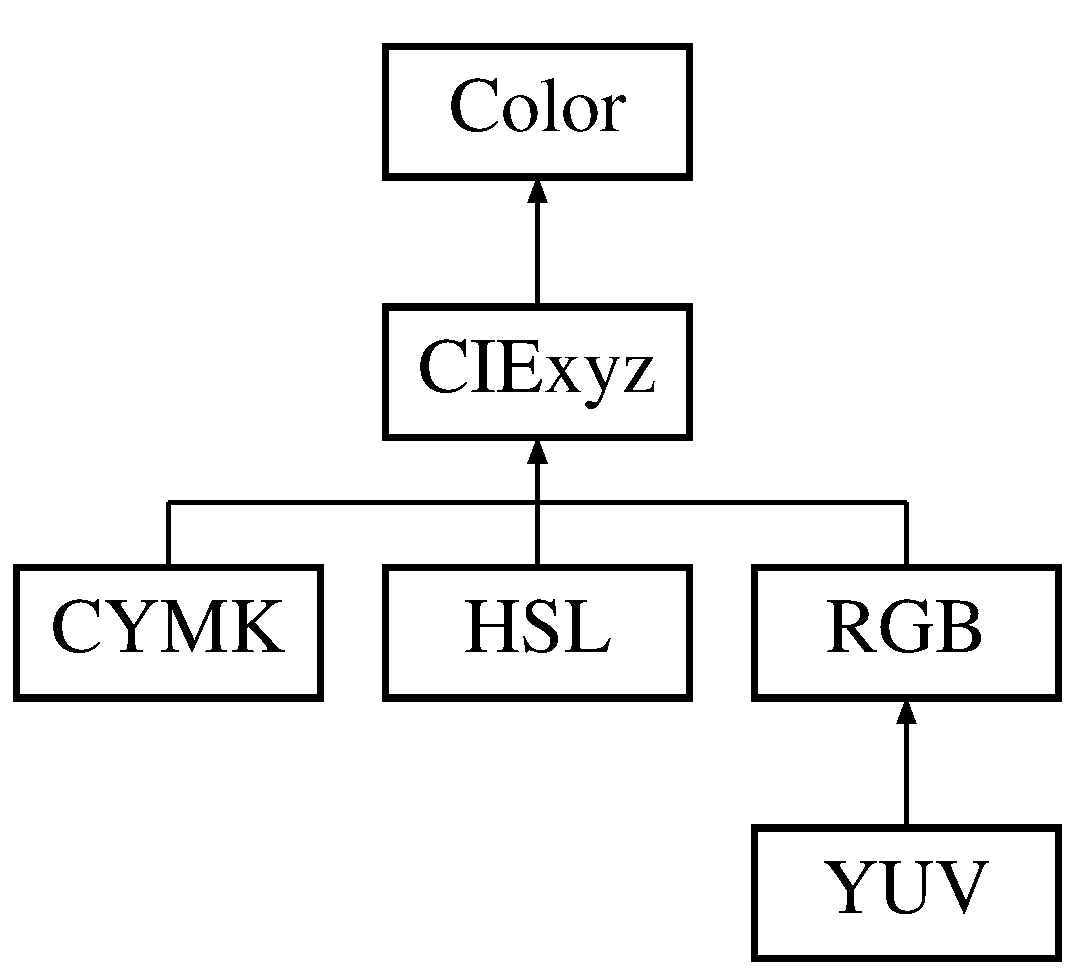
\includegraphics[height=4.000000cm]{class_c_i_exyz}
\end{center}
\end{figure}
\subsection*{Public Member Functions}
\begin{DoxyCompactItemize}
\item 
\hyperlink{class_c_i_exyz_aea8a8b567ac89a96b0bf4c749a49ea90}{C\+I\+Exyz} (double t\+\_\+x=0, double t\+\_\+y=0, double t\+\_\+z=0)
\begin{DoxyCompactList}\small\item\em \hyperlink{class_c_i_exyz_aea8a8b567ac89a96b0bf4c749a49ea90}{C\+I\+Exyz\+::\+C\+I\+Exyz} Constructor for C\+IE xyz color representation from double precision numbers. \end{DoxyCompactList}\item 
\hyperlink{class_c_i_exyz_aa16b12dfc4f0ceac557778e5bede454c}{C\+I\+Exyz} (const \hyperlink{class_c_i_exyz}{C\+I\+Exyz} \&c)
\begin{DoxyCompactList}\small\item\em \hyperlink{class_c_i_exyz_aea8a8b567ac89a96b0bf4c749a49ea90}{C\+I\+Exyz\+::\+C\+I\+Exyz} copy constructor. \end{DoxyCompactList}\item 
\hyperlink{class_c_i_exyz_a861692ec98ae70d205cbee47fc63a879}{C\+I\+Exyz} (const \hyperlink{class_color}{Color} $\ast$c)
\begin{DoxyCompactList}\small\item\em \hyperlink{class_c_i_exyz_aea8a8b567ac89a96b0bf4c749a49ea90}{C\+I\+Exyz\+::\+C\+I\+Exyz} constructor for C\+IE xyz color representation from \hyperlink{class_color}{Color} pointer in the same color space. \end{DoxyCompactList}\item 
int \hyperlink{class_c_i_exyz_af168733bb1bca36a7ae5d75c67de046e}{get\+Number\+Of\+Componets} () const
\begin{DoxyCompactList}\small\item\em \hyperlink{class_c_i_exyz_af168733bb1bca36a7ae5d75c67de046e}{C\+I\+Exyz\+::get\+Number\+Of\+Componets}. \end{DoxyCompactList}\item 
Q\+Vector$<$ Q\+String $>$ \hyperlink{class_c_i_exyz_a4c3aa6777f7720ae26b53174322a83f8}{get\+Limits} () const
\begin{DoxyCompactList}\small\item\em \hyperlink{class_c_i_exyz_a4c3aa6777f7720ae26b53174322a83f8}{C\+I\+Exyz\+::get\+Limits}. \end{DoxyCompactList}\item 
void \hyperlink{class_c_i_exyz_a11468574f91d2cb1356f0cde56429b84}{set\+Components} (Q\+Vector$<$ double $>$ componets)
\begin{DoxyCompactList}\small\item\em \hyperlink{class_c_i_exyz_a11468574f91d2cb1356f0cde56429b84}{C\+I\+Exyz\+::set\+Components} set the components inside the object. \end{DoxyCompactList}\item 
Q\+String \hyperlink{class_c_i_exyz_a19120c15d1304696909d76fae6065ebd}{get\+Representation} () const
\begin{DoxyCompactList}\small\item\em C\+I\+Exyz\+::getrepresentation. \end{DoxyCompactList}\item 
\hyperlink{class_color}{Color} $\ast$ \hyperlink{class_c_i_exyz_a4a454df6cbb71f3fcfd2d1ea9d500d94}{negate} () const
\begin{DoxyCompactList}\small\item\em \hyperlink{class_c_i_exyz_a4a454df6cbb71f3fcfd2d1ea9d500d94}{C\+I\+Exyz\+::negate}. \end{DoxyCompactList}\item 
\hyperlink{class_color}{Color} $\ast$ \hyperlink{class_c_i_exyz_af8eeb48ade44beea43d023b36d263fc8}{mix} (const \hyperlink{class_color}{Color} $\ast$c) const
\begin{DoxyCompactList}\small\item\em \hyperlink{class_c_i_exyz_af8eeb48ade44beea43d023b36d263fc8}{C\+I\+Exyz\+::mix}. \end{DoxyCompactList}\item 
\hyperlink{class_color}{Color} $\ast$ \hyperlink{class_c_i_exyz_aa93c7a293b63c7bce8d1fab9a185ab1b}{get\+C\+IE} () const
\begin{DoxyCompactList}\small\item\em \hyperlink{class_c_i_exyz_aa93c7a293b63c7bce8d1fab9a185ab1b}{C\+I\+Exyz\+::get\+C\+IE}. \end{DoxyCompactList}\item 
\hyperlink{class_color}{Color} $\ast$ \hyperlink{class_c_i_exyz_abb3f5e1c8a923d7758e6bbe83b71f4fa}{operator/} (const int \&div) const
\begin{DoxyCompactList}\small\item\em \hyperlink{class_c_i_exyz_abb3f5e1c8a923d7758e6bbe83b71f4fa}{C\+I\+Exyz\+::operator /}. \end{DoxyCompactList}\item 
Q\+Vector$<$ Q\+String $>$ \hyperlink{class_c_i_exyz_aa82a27c78ff425e06cdd740dd50e93b1}{available\+Operations} () const
\begin{DoxyCompactList}\small\item\em \hyperlink{class_c_i_exyz_aa82a27c78ff425e06cdd740dd50e93b1}{C\+I\+Exyz\+::available\+Operations}. \end{DoxyCompactList}\item 
Q\+Vector$<$ double $>$ \hyperlink{class_c_i_exyz_af8992e3ac1741c35fcb18aa2cdb554a0}{get\+Components} () const
\begin{DoxyCompactList}\small\item\em C\+I\+Exyz\+::get\+Component. \end{DoxyCompactList}\end{DoxyCompactItemize}
\subsection*{Additional Inherited Members}


\subsection{Detailed Description}
this class uses the base class \hyperlink{class_color}{Color} and implements a C\+IE xyz color space in D65 white point \hyperlink{class_c_i_exyz}{C\+I\+Exyz} stores a color in C\+IE xyz whit a d65 white point representation 

\subsection{Constructor \& Destructor Documentation}
\mbox{\Hypertarget{class_c_i_exyz_aea8a8b567ac89a96b0bf4c749a49ea90}\label{class_c_i_exyz_aea8a8b567ac89a96b0bf4c749a49ea90}} 
\index{C\+I\+Exyz@{C\+I\+Exyz}!C\+I\+Exyz@{C\+I\+Exyz}}
\index{C\+I\+Exyz@{C\+I\+Exyz}!C\+I\+Exyz@{C\+I\+Exyz}}
\subsubsection{\texorpdfstring{C\+I\+Exyz()}{CIExyz()}\hspace{0.1cm}{\footnotesize\ttfamily [1/3]}}
{\footnotesize\ttfamily C\+I\+Exyz\+::\+C\+I\+Exyz (\begin{DoxyParamCaption}\item[{double}]{t\+\_\+x = {\ttfamily 0},  }\item[{double}]{t\+\_\+y = {\ttfamily 0},  }\item[{double}]{t\+\_\+z = {\ttfamily 0} }\end{DoxyParamCaption})}



\hyperlink{class_c_i_exyz_aea8a8b567ac89a96b0bf4c749a49ea90}{C\+I\+Exyz\+::\+C\+I\+Exyz} Constructor for C\+IE xyz color representation from double precision numbers. 


\begin{DoxyParams}{Parameters}
{\em t\+\_\+x} & \\
\hline
{\em t\+\_\+y} & \\
\hline
{\em t\+\_\+z} & \\
\hline
\end{DoxyParams}

\begin{DoxyExceptions}{Exceptions}
{\em \hyperlink{class_illegal_color_exception}{Illegal\+Color\+Exception}} & \\
\hline
\end{DoxyExceptions}
\mbox{\Hypertarget{class_c_i_exyz_aa16b12dfc4f0ceac557778e5bede454c}\label{class_c_i_exyz_aa16b12dfc4f0ceac557778e5bede454c}} 
\index{C\+I\+Exyz@{C\+I\+Exyz}!C\+I\+Exyz@{C\+I\+Exyz}}
\index{C\+I\+Exyz@{C\+I\+Exyz}!C\+I\+Exyz@{C\+I\+Exyz}}
\subsubsection{\texorpdfstring{C\+I\+Exyz()}{CIExyz()}\hspace{0.1cm}{\footnotesize\ttfamily [2/3]}}
{\footnotesize\ttfamily C\+I\+Exyz\+::\+C\+I\+Exyz (\begin{DoxyParamCaption}\item[{const \hyperlink{class_c_i_exyz}{C\+I\+Exyz} \&}]{c }\end{DoxyParamCaption})}



\hyperlink{class_c_i_exyz_aea8a8b567ac89a96b0bf4c749a49ea90}{C\+I\+Exyz\+::\+C\+I\+Exyz} copy constructor. 


\begin{DoxyParams}{Parameters}
{\em c} & \\
\hline
\end{DoxyParams}
\mbox{\Hypertarget{class_c_i_exyz_a861692ec98ae70d205cbee47fc63a879}\label{class_c_i_exyz_a861692ec98ae70d205cbee47fc63a879}} 
\index{C\+I\+Exyz@{C\+I\+Exyz}!C\+I\+Exyz@{C\+I\+Exyz}}
\index{C\+I\+Exyz@{C\+I\+Exyz}!C\+I\+Exyz@{C\+I\+Exyz}}
\subsubsection{\texorpdfstring{C\+I\+Exyz()}{CIExyz()}\hspace{0.1cm}{\footnotesize\ttfamily [3/3]}}
{\footnotesize\ttfamily C\+I\+Exyz\+::\+C\+I\+Exyz (\begin{DoxyParamCaption}\item[{const \hyperlink{class_color}{Color} $\ast$}]{c }\end{DoxyParamCaption})}



\hyperlink{class_c_i_exyz_aea8a8b567ac89a96b0bf4c749a49ea90}{C\+I\+Exyz\+::\+C\+I\+Exyz} constructor for C\+IE xyz color representation from \hyperlink{class_color}{Color} pointer in the same color space. 


\begin{DoxyExceptions}{Exceptions}
{\em \hyperlink{class_illegal_color_exception}{Illegal\+Color\+Exception}} & \\
\hline
\end{DoxyExceptions}

\begin{DoxyParams}{Parameters}
{\em c} & \\
\hline
\end{DoxyParams}


\subsection{Member Function Documentation}
\mbox{\Hypertarget{class_c_i_exyz_aa82a27c78ff425e06cdd740dd50e93b1}\label{class_c_i_exyz_aa82a27c78ff425e06cdd740dd50e93b1}} 
\index{C\+I\+Exyz@{C\+I\+Exyz}!available\+Operations@{available\+Operations}}
\index{available\+Operations@{available\+Operations}!C\+I\+Exyz@{C\+I\+Exyz}}
\subsubsection{\texorpdfstring{available\+Operations()}{availableOperations()}}
{\footnotesize\ttfamily Q\+Vector$<$ Q\+String $>$ C\+I\+Exyz\+::available\+Operations (\begin{DoxyParamCaption}{ }\end{DoxyParamCaption}) const\hspace{0.3cm}{\ttfamily [virtual]}}



\hyperlink{class_c_i_exyz_aa82a27c78ff425e06cdd740dd50e93b1}{C\+I\+Exyz\+::available\+Operations}. 

\begin{DoxyReturn}{Returns}
all the operation that has been implemented 
\end{DoxyReturn}


Implements \hyperlink{class_color}{Color}.



Reimplemented in \hyperlink{class_r_g_b_a6cde5a9d00036c76fef2dd51ca8256a4}{R\+GB}.

\mbox{\Hypertarget{class_c_i_exyz_aa93c7a293b63c7bce8d1fab9a185ab1b}\label{class_c_i_exyz_aa93c7a293b63c7bce8d1fab9a185ab1b}} 
\index{C\+I\+Exyz@{C\+I\+Exyz}!get\+C\+IE@{get\+C\+IE}}
\index{get\+C\+IE@{get\+C\+IE}!C\+I\+Exyz@{C\+I\+Exyz}}
\subsubsection{\texorpdfstring{get\+C\+I\+E()}{getCIE()}}
{\footnotesize\ttfamily \hyperlink{class_color}{Color} $\ast$ C\+I\+Exyz\+::get\+C\+IE (\begin{DoxyParamCaption}{ }\end{DoxyParamCaption}) const\hspace{0.3cm}{\ttfamily [virtual]}}



\hyperlink{class_c_i_exyz_aa93c7a293b63c7bce8d1fab9a185ab1b}{C\+I\+Exyz\+::get\+C\+IE}. 

\begin{DoxyReturn}{Returns}
\hyperlink{class_color}{Color} pointer with a clone of $\ast$this 
\end{DoxyReturn}


Implements \hyperlink{class_color}{Color}.



Reimplemented in \hyperlink{class_r_g_b_ac4b085d5587c664f7f9ceae1eb857d24}{R\+GB}.

\mbox{\Hypertarget{class_c_i_exyz_af8992e3ac1741c35fcb18aa2cdb554a0}\label{class_c_i_exyz_af8992e3ac1741c35fcb18aa2cdb554a0}} 
\index{C\+I\+Exyz@{C\+I\+Exyz}!get\+Components@{get\+Components}}
\index{get\+Components@{get\+Components}!C\+I\+Exyz@{C\+I\+Exyz}}
\subsubsection{\texorpdfstring{get\+Components()}{getComponents()}}
{\footnotesize\ttfamily Q\+Vector$<$ double $>$ C\+I\+Exyz\+::get\+Components (\begin{DoxyParamCaption}{ }\end{DoxyParamCaption}) const\hspace{0.3cm}{\ttfamily [virtual]}}



C\+I\+Exyz\+::get\+Component. 

\begin{DoxyReturn}{Returns}
Q\+Vector$<$double$>$ with the x y z component of the color in C\+IE X\+YZ 
\end{DoxyReturn}


Implements \hyperlink{class_color}{Color}.



Reimplemented in \hyperlink{class_r_g_b_ad085d3bd654d874ea2e5739a5c216769}{R\+GB}, \hyperlink{class_c_y_m_k_a46e1058b0332d73710efa5d9f4644ba2}{C\+Y\+MK}, \hyperlink{class_h_s_l_a2de2eb4fa5c9ffcea894f7c6591cb335}{H\+SL}, and \hyperlink{class_y_u_v_ad90109db3486e61e248e274a7690824a}{Y\+UV}.

\mbox{\Hypertarget{class_c_i_exyz_a4c3aa6777f7720ae26b53174322a83f8}\label{class_c_i_exyz_a4c3aa6777f7720ae26b53174322a83f8}} 
\index{C\+I\+Exyz@{C\+I\+Exyz}!get\+Limits@{get\+Limits}}
\index{get\+Limits@{get\+Limits}!C\+I\+Exyz@{C\+I\+Exyz}}
\subsubsection{\texorpdfstring{get\+Limits()}{getLimits()}}
{\footnotesize\ttfamily Q\+Vector$<$ Q\+String $>$ C\+I\+Exyz\+::get\+Limits (\begin{DoxyParamCaption}{ }\end{DoxyParamCaption}) const\hspace{0.3cm}{\ttfamily [virtual]}}



\hyperlink{class_c_i_exyz_a4c3aa6777f7720ae26b53174322a83f8}{C\+I\+Exyz\+::get\+Limits}. 

\begin{DoxyReturn}{Returns}
limits as Q\+Vector$<$\+Q\+String$>$ 
\end{DoxyReturn}


Implements \hyperlink{class_color}{Color}.



Reimplemented in \hyperlink{class_r_g_b_a4ae8d5c061e45f557a5924f2237c1d0e}{R\+GB}, \hyperlink{class_y_u_v_a344cd573b663c97f5554afcb1c15458c}{Y\+UV}, \hyperlink{class_c_y_m_k_a9e0f2df82394cab1f95782f381c560ab}{C\+Y\+MK}, and \hyperlink{class_h_s_l_a7ac26d7b7b5755769165455e1b6d3312}{H\+SL}.

\mbox{\Hypertarget{class_c_i_exyz_af168733bb1bca36a7ae5d75c67de046e}\label{class_c_i_exyz_af168733bb1bca36a7ae5d75c67de046e}} 
\index{C\+I\+Exyz@{C\+I\+Exyz}!get\+Number\+Of\+Componets@{get\+Number\+Of\+Componets}}
\index{get\+Number\+Of\+Componets@{get\+Number\+Of\+Componets}!C\+I\+Exyz@{C\+I\+Exyz}}
\subsubsection{\texorpdfstring{get\+Number\+Of\+Componets()}{getNumberOfComponets()}}
{\footnotesize\ttfamily int C\+I\+Exyz\+::get\+Number\+Of\+Componets (\begin{DoxyParamCaption}{ }\end{DoxyParamCaption}) const\hspace{0.3cm}{\ttfamily [virtual]}}



\hyperlink{class_c_i_exyz_af168733bb1bca36a7ae5d75c67de046e}{C\+I\+Exyz\+::get\+Number\+Of\+Componets}. 

\begin{DoxyReturn}{Returns}
number of componets 
\end{DoxyReturn}


Implements \hyperlink{class_color}{Color}.



Reimplemented in \hyperlink{class_r_g_b_a7561d57d6706bc25ea10762d906b2345}{R\+GB}, \hyperlink{class_c_y_m_k_ab3f005a1cc28f715192ad4fc90ded6b8}{C\+Y\+MK}, \hyperlink{class_h_s_l_a6e582f5779c1b5f84abe8bb182a868d0}{H\+SL}, and \hyperlink{class_y_u_v_a46eded5c13a0c2b2e9bbf05d4a2f9c7c}{Y\+UV}.

\mbox{\Hypertarget{class_c_i_exyz_a19120c15d1304696909d76fae6065ebd}\label{class_c_i_exyz_a19120c15d1304696909d76fae6065ebd}} 
\index{C\+I\+Exyz@{C\+I\+Exyz}!get\+Representation@{get\+Representation}}
\index{get\+Representation@{get\+Representation}!C\+I\+Exyz@{C\+I\+Exyz}}
\subsubsection{\texorpdfstring{get\+Representation()}{getRepresentation()}}
{\footnotesize\ttfamily Q\+String C\+I\+Exyz\+::get\+Representation (\begin{DoxyParamCaption}{ }\end{DoxyParamCaption}) const\hspace{0.3cm}{\ttfamily [virtual]}}



C\+I\+Exyz\+::getrepresentation. 

\begin{DoxyReturn}{Returns}
Q\+String that contains name of the object 
\end{DoxyReturn}


Implements \hyperlink{class_color}{Color}.



Reimplemented in \hyperlink{class_r_g_b_a5f7a68904e1e4f18c22c1066170fb2bf}{R\+GB}, \hyperlink{class_c_y_m_k_aa523f734fd52f67ca9fcb31f0b7fe579}{C\+Y\+MK}, \hyperlink{class_h_s_l_a774dc0a5dad87bc9ff44956af4873602}{H\+SL}, and \hyperlink{class_y_u_v_ae38403ffd397003eb28ab7670f95d1e5}{Y\+UV}.

\mbox{\Hypertarget{class_c_i_exyz_af8eeb48ade44beea43d023b36d263fc8}\label{class_c_i_exyz_af8eeb48ade44beea43d023b36d263fc8}} 
\index{C\+I\+Exyz@{C\+I\+Exyz}!mix@{mix}}
\index{mix@{mix}!C\+I\+Exyz@{C\+I\+Exyz}}
\subsubsection{\texorpdfstring{mix()}{mix()}}
{\footnotesize\ttfamily \hyperlink{class_color}{Color} $\ast$ C\+I\+Exyz\+::mix (\begin{DoxyParamCaption}\item[{const \hyperlink{class_color}{Color} $\ast$}]{c }\end{DoxyParamCaption}) const\hspace{0.3cm}{\ttfamily [virtual]}}



\hyperlink{class_c_i_exyz_af8eeb48ade44beea43d023b36d263fc8}{C\+I\+Exyz\+::mix}. 


\begin{DoxyParams}{Parameters}
{\em c} & \\
\hline
\end{DoxyParams}
\begin{DoxyReturn}{Returns}
\hyperlink{class_color}{Color} pointer with a new color mixed 
\end{DoxyReturn}


Implements \hyperlink{class_color}{Color}.



Reimplemented in \hyperlink{class_r_g_b_aa022866e33474ab64f81d367c6b030b9}{R\+GB}, \hyperlink{class_c_y_m_k_adeb4691eafbb53e15538a3d829f59a14}{C\+Y\+MK}, \hyperlink{class_h_s_l_a08bcec2ca6961b7c6431d92a625c30a7}{H\+SL}, and \hyperlink{class_y_u_v_ab152a4ea37eaa67df0b38882c2099da3}{Y\+UV}.

\mbox{\Hypertarget{class_c_i_exyz_a4a454df6cbb71f3fcfd2d1ea9d500d94}\label{class_c_i_exyz_a4a454df6cbb71f3fcfd2d1ea9d500d94}} 
\index{C\+I\+Exyz@{C\+I\+Exyz}!negate@{negate}}
\index{negate@{negate}!C\+I\+Exyz@{C\+I\+Exyz}}
\subsubsection{\texorpdfstring{negate()}{negate()}}
{\footnotesize\ttfamily \hyperlink{class_color}{Color} $\ast$ C\+I\+Exyz\+::negate (\begin{DoxyParamCaption}{ }\end{DoxyParamCaption}) const\hspace{0.3cm}{\ttfamily [virtual]}}



\hyperlink{class_c_i_exyz_a4a454df6cbb71f3fcfd2d1ea9d500d94}{C\+I\+Exyz\+::negate}. 

\begin{DoxyReturn}{Returns}
\hyperlink{class_color}{Color} pointer with a new color with the negated values 
\end{DoxyReturn}


Implements \hyperlink{class_color}{Color}.



Reimplemented in \hyperlink{class_r_g_b_a7aad38ac17ec3201c65f8f5e90637b69}{R\+GB}, \hyperlink{class_c_y_m_k_a397c0109e76ff6cc331b49e4b73623ef}{C\+Y\+MK}, \hyperlink{class_h_s_l_af681f885d11220b0588e8f969aa95e32}{H\+SL}, and \hyperlink{class_y_u_v_a079872ae88552066ce1abb39cc0a40de}{Y\+UV}.

\mbox{\Hypertarget{class_c_i_exyz_abb3f5e1c8a923d7758e6bbe83b71f4fa}\label{class_c_i_exyz_abb3f5e1c8a923d7758e6bbe83b71f4fa}} 
\index{C\+I\+Exyz@{C\+I\+Exyz}!operator/@{operator/}}
\index{operator/@{operator/}!C\+I\+Exyz@{C\+I\+Exyz}}
\subsubsection{\texorpdfstring{operator/()}{operator/()}}
{\footnotesize\ttfamily \hyperlink{class_color}{Color} $\ast$ C\+I\+Exyz\+::operator/ (\begin{DoxyParamCaption}\item[{const int \&}]{div }\end{DoxyParamCaption}) const\hspace{0.3cm}{\ttfamily [virtual]}}



\hyperlink{class_c_i_exyz_abb3f5e1c8a923d7758e6bbe83b71f4fa}{C\+I\+Exyz\+::operator /}. 


\begin{DoxyExceptions}{Exceptions}
{\em \hyperlink{class_illegal_color_exception}{Illegal\+Color\+Exception}} & \\
\hline
\end{DoxyExceptions}


Implements \hyperlink{class_color}{Color}.



Reimplemented in \hyperlink{class_r_g_b_a9d250e0f58e7ae7d4c69ced724da6f80}{R\+GB}, and \hyperlink{class_y_u_v_a1b9300c00323eca16fc4bb028964e85f}{Y\+UV}.

\mbox{\Hypertarget{class_c_i_exyz_a11468574f91d2cb1356f0cde56429b84}\label{class_c_i_exyz_a11468574f91d2cb1356f0cde56429b84}} 
\index{C\+I\+Exyz@{C\+I\+Exyz}!set\+Components@{set\+Components}}
\index{set\+Components@{set\+Components}!C\+I\+Exyz@{C\+I\+Exyz}}
\subsubsection{\texorpdfstring{set\+Components()}{setComponents()}}
{\footnotesize\ttfamily void C\+I\+Exyz\+::set\+Components (\begin{DoxyParamCaption}\item[{Q\+Vector$<$ double $>$}]{componets }\end{DoxyParamCaption})\hspace{0.3cm}{\ttfamily [virtual]}}



\hyperlink{class_c_i_exyz_a11468574f91d2cb1356f0cde56429b84}{C\+I\+Exyz\+::set\+Components} set the components inside the object. 


\begin{DoxyExceptions}{Exceptions}
{\em \hyperlink{class_illegal_color_exception}{Illegal\+Color\+Exception}} & \\
\hline
\end{DoxyExceptions}

\begin{DoxyParams}{Parameters}
{\em componets} & with 3 values xyz \\
\hline
\end{DoxyParams}


Implements \hyperlink{class_color}{Color}.



Reimplemented in \hyperlink{class_c_y_m_k_a897a2a1030cfd10dc16d5e2de825b45e}{C\+Y\+MK}, \hyperlink{class_r_g_b_acf213178f2029a5f304d62b87dbb6b36}{R\+GB}, \hyperlink{class_y_u_v_a622daf7a688da4a227b63deb412c0d46}{Y\+UV}, and \hyperlink{class_h_s_l_a101be14729707abca388680610e2fe86}{H\+SL}.



The documentation for this class was generated from the following files\+:\begin{DoxyCompactItemize}
\item 
/home/gian/\+Projects/\+Kalk2-\/0/\+Kalk/\+Model/\+Color/\+C\+I\+E\+\_\+xyz/cie\+\_\+xyz.\+h\item 
/home/gian/\+Projects/\+Kalk2-\/0/\+Kalk/\+Model/\+Color/\+C\+I\+E\+\_\+xyz/cie\+\_\+xyz.\+cpp\end{DoxyCompactItemize}

\hypertarget{class_color}{}\section{Color Class Reference}
\label{class_color}\index{Color@{Color}}


this class is the main base for color representation in this program  




{\ttfamily \#include $<$color.\+h$>$}

Inheritance diagram for Color\+:\begin{figure}[H]
\begin{center}
\leavevmode
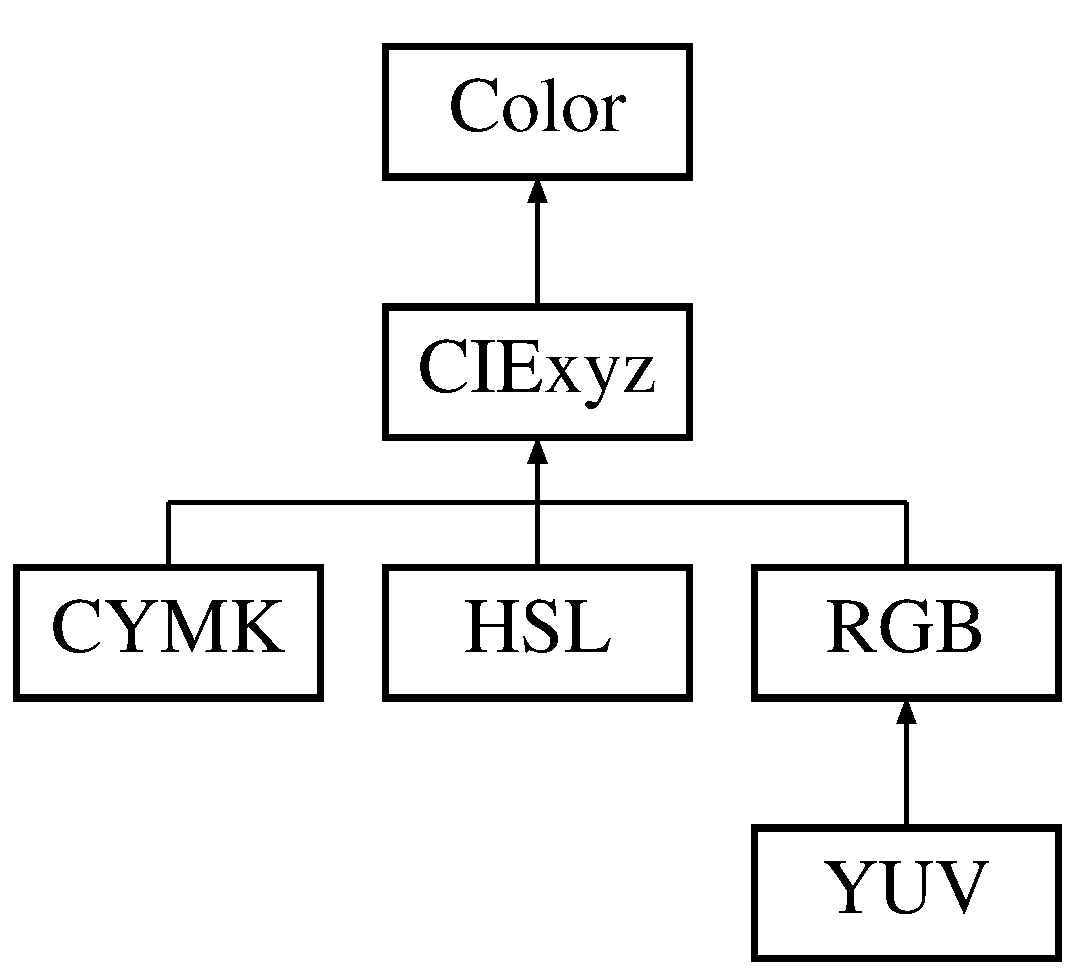
\includegraphics[height=4.000000cm]{class_color}
\end{center}
\end{figure}
\subsection*{Public Member Functions}
\begin{DoxyCompactItemize}
\item 
\mbox{\Hypertarget{class_color_a0e16ae80374851824e791a941c6315e1}\label{class_color_a0e16ae80374851824e791a941c6315e1}} 
virtual int {\bfseries get\+Number\+Of\+Componets} () const =0
\item 
\mbox{\Hypertarget{class_color_a84ee279d59516539f2940a424018c376}\label{class_color_a84ee279d59516539f2940a424018c376}} 
virtual void {\bfseries set\+Components} (Q\+Vector$<$ double $>$ componets)=0
\item 
\mbox{\Hypertarget{class_color_a5d360ee273c34bceb8dd5837489a0a18}\label{class_color_a5d360ee273c34bceb8dd5837489a0a18}} 
virtual \hyperlink{class_color}{Color} $\ast$ {\bfseries get\+C\+IE} () const =0
\item 
\mbox{\Hypertarget{class_color_aa73035295e3e42593b11904c398f1657}\label{class_color_aa73035295e3e42593b11904c398f1657}} 
virtual \hyperlink{class_color}{Color} $\ast$ {\bfseries negate} () const =0
\item 
\mbox{\Hypertarget{class_color_ab240ddb0e1d4779703f6b2ee35a8a0e9}\label{class_color_ab240ddb0e1d4779703f6b2ee35a8a0e9}} 
virtual \hyperlink{class_color}{Color} $\ast$ {\bfseries mix} (const \hyperlink{class_color}{Color} $\ast$c1) const =0
\item 
\mbox{\Hypertarget{class_color_acb25591213c391f682c9261c85dc111c}\label{class_color_acb25591213c391f682c9261c85dc111c}} 
virtual \hyperlink{class_color}{Color} $\ast$ {\bfseries operator/} (const int \&div) const =0
\item 
\mbox{\Hypertarget{class_color_a4880c6f39c155008b711c056b21ff31b}\label{class_color_a4880c6f39c155008b711c056b21ff31b}} 
virtual Q\+Vector$<$ Q\+String $>$ {\bfseries get\+Limits} () const =0
\item 
\mbox{\Hypertarget{class_color_af521a40fabd5e4718ada6531fc20ec58}\label{class_color_af521a40fabd5e4718ada6531fc20ec58}} 
virtual Q\+Vector$<$ Q\+String $>$ {\bfseries available\+Operations} () const =0
\item 
\mbox{\Hypertarget{class_color_a0c30989b24589c8725abe286cc5e7a23}\label{class_color_a0c30989b24589c8725abe286cc5e7a23}} 
virtual Q\+Vector$<$ double $>$ {\bfseries get\+Components} () const =0
\item 
\mbox{\Hypertarget{class_color_a45ec07f1486ab8259cdd8630c804b9f6}\label{class_color_a45ec07f1486ab8259cdd8630c804b9f6}} 
virtual Q\+String {\bfseries get\+Representation} () const =0
\end{DoxyCompactItemize}
\subsection*{Static Public Attributes}
\begin{DoxyCompactItemize}
\item 
\mbox{\Hypertarget{class_color_af49cd7836a808e9e36408f996ea3ce0e}\label{class_color_af49cd7836a808e9e36408f996ea3ce0e}} 
static const Q\+String {\bfseries all\+Opts} \mbox{[}3\mbox{]}\mbox{[}3\mbox{]} =\{\{\char`\"{}negate\char`\"{},\char`\"{}non disponibile\char`\"{},\char`\"{}\char`\"{}\},\{\char`\"{}mix\char`\"{},\char`\"{}color\char`\"{},\char`\"{}\char`\"{}\},\{\char`\"{}divide\char`\"{},\char`\"{}intero\char`\"{},\char`\"{}\char`\"{}\}\}
\end{DoxyCompactItemize}


\subsection{Detailed Description}
this class is the main base for color representation in this program 

The documentation for this class was generated from the following files\+:\begin{DoxyCompactItemize}
\item 
/home/gian/\+Projects/\+Kalk2-\/0/\+Kalk/\+Model/\+Color/color.\+h\item 
/home/gian/\+Projects/\+Kalk2-\/0/\+Kalk/\+Model/\+Color/color.\+cpp\end{DoxyCompactItemize}

\hypertarget{class_color_factory}{}\section{Color\+Factory Class Reference}
\label{class_color_factory}\index{Color\+Factory@{Color\+Factory}}


this class stores all Factories, \hyperlink{class_color_factory}{Color\+Factory} initializes a New \hyperlink{class_color}{Color} object when required, returns what kind of operation can be done with a specific color representation and returns the result using the permitted operations  




{\ttfamily \#include $<$colorfactory.\+h$>$}

\subsection*{Static Public Member Functions}
\begin{DoxyCompactItemize}
\item 
\mbox{\Hypertarget{class_color_factory_ad47298cad09cd5d2eb52c801354f5c8e}\label{class_color_factory_ad47298cad09cd5d2eb52c801354f5c8e}} 
static void \hyperlink{class_color_factory_ad47298cad09cd5d2eb52c801354f5c8e}{set\+Up\+Color\+Factory} ()
\begin{DoxyCompactList}\small\item\em \hyperlink{class_color_factory_ad47298cad09cd5d2eb52c801354f5c8e}{Color\+Factory\+::set\+Up\+Color\+Factory} Setups the data structure to be populated by add\+Color\+Factory. \end{DoxyCompactList}\item 
\mbox{\Hypertarget{class_color_factory_a99c58dc4bb1d431f1a7c399fec9d2486}\label{class_color_factory_a99c58dc4bb1d431f1a7c399fec9d2486}} 
static void \hyperlink{class_color_factory_a99c58dc4bb1d431f1a7c399fec9d2486}{destruct} ()
\begin{DoxyCompactList}\small\item\em \hyperlink{class_color_factory_a99c58dc4bb1d431f1a7c399fec9d2486}{Color\+Factory\+::destruct} deletes all data from all\+Color\+Factories;. \end{DoxyCompactList}\item 
static bool \hyperlink{class_color_factory_a998d381b54b7b74ca24a99593030a452}{ready} ()
\begin{DoxyCompactList}\small\item\em \hyperlink{class_color_factory_a998d381b54b7b74ca24a99593030a452}{Color\+Factory\+::ready}. \end{DoxyCompactList}\item 
static void \hyperlink{class_color_factory_a16fd150054d514e72eaf6d5bf9e80fe2}{add\+Color\+Factory} (const Q\+String \&name, \hyperlink{class_generic_factory}{Generic\+Factory} \&factory)
\begin{DoxyCompactList}\small\item\em \hyperlink{class_color_factory_a16fd150054d514e72eaf6d5bf9e80fe2}{Color\+Factory\+::add\+Color\+Factory}. \end{DoxyCompactList}\item 
static Q\+Vector$<$ Q\+String $>$ \hyperlink{class_color_factory_a47dab64f01e0d5543ed41d82742b1a32}{get\+All\+Color\+Types} ()
\begin{DoxyCompactList}\small\item\em \hyperlink{class_color_factory_a47dab64f01e0d5543ed41d82742b1a32}{Color\+Factory\+::get\+All\+Color\+Types}. \end{DoxyCompactList}\item 
static \hyperlink{class_color}{Color} $\ast$ \hyperlink{class_color_factory_a0b8412fa33dd5eaefff38412a96fc638}{get\+New\+Color} (const Q\+String \&key)
\begin{DoxyCompactList}\small\item\em \hyperlink{class_color_factory_a0b8412fa33dd5eaefff38412a96fc638}{Color\+Factory\+::get\+New\+Color}. \end{DoxyCompactList}\item 
static \hyperlink{class_color}{Color} $\ast$ \hyperlink{class_color_factory_a1fcc2e8e07462cd0932317144c712c86}{get\+New\+Color} (const Q\+String \&key, const \hyperlink{class_color}{Color} $\ast$color)
\begin{DoxyCompactList}\small\item\em \hyperlink{class_color_factory_a0b8412fa33dd5eaefff38412a96fc638}{Color\+Factory\+::get\+New\+Color}. \end{DoxyCompactList}\item 
static \hyperlink{class_color}{Color} $\ast$ \hyperlink{class_color_factory_a2c20174b2a883ee984ddb21d4cb31b5f}{clone\+Color} (const \hyperlink{class_color}{Color} $\ast$color)
\begin{DoxyCompactList}\small\item\em \hyperlink{class_color_factory_a2c20174b2a883ee984ddb21d4cb31b5f}{Color\+Factory\+::clone\+Color}. \end{DoxyCompactList}\item 
static \hyperlink{class_color}{Color} $\ast$ \hyperlink{class_color_factory_a011ad08eec6d8b4f6e8bba6da64ec345}{execution} (const \hyperlink{class_color}{Color} $\ast$left, int operation, const \hyperlink{class_color}{Color} $\ast$right=nullptr)
\begin{DoxyCompactList}\small\item\em \hyperlink{class_color_factory_a011ad08eec6d8b4f6e8bba6da64ec345}{Color\+Factory\+::execution}. \end{DoxyCompactList}\item 
static \hyperlink{class_color}{Color} $\ast$ \hyperlink{class_color_factory_a35ec83ba9159727511989055e7868d63}{execution} (const \hyperlink{class_color}{Color} $\ast$left, const int \&operation, const int right=1)
\begin{DoxyCompactList}\small\item\em \hyperlink{class_color_factory_a011ad08eec6d8b4f6e8bba6da64ec345}{Color\+Factory\+::execution}. \end{DoxyCompactList}\item 
static Q\+Vector$<$ Q\+String $>$ \hyperlink{class_color_factory_a9dc30325232e3cf63276ed8f9c2d6ab1}{available\+Operations} ()
\begin{DoxyCompactList}\small\item\em \hyperlink{class_color_factory_a9dc30325232e3cf63276ed8f9c2d6ab1}{Color\+Factory\+::available\+Operations}. \end{DoxyCompactList}\item 
static Q\+Vector$<$ Q\+String $>$ \hyperlink{class_color_factory_a4a6862d52370ea64981f1842dfa6c4f2}{permitted\+Operations} (const Q\+String \&type)
\begin{DoxyCompactList}\small\item\em \hyperlink{class_color_factory_a4a6862d52370ea64981f1842dfa6c4f2}{Color\+Factory\+::permitted\+Operations}. \end{DoxyCompactList}\item 
static Q\+Vector$<$ Q\+String $>$ \hyperlink{class_color_factory_a460165d3cd7b710b4f8731a5e56d8c35}{type\+By\+Operation} (int operation)
\begin{DoxyCompactList}\small\item\em \hyperlink{class_color_factory_a460165d3cd7b710b4f8731a5e56d8c35}{Color\+Factory\+::type\+By\+Operation}. \end{DoxyCompactList}\item 
\mbox{\Hypertarget{class_color_factory_a08c21c5ec305802deb7d610ff0a66ef7}\label{class_color_factory_a08c21c5ec305802deb7d610ff0a66ef7}} 
static int {\bfseries get\+Type\+Size} ()
\end{DoxyCompactItemize}


\subsection{Detailed Description}
this class stores all Factories, \hyperlink{class_color_factory}{Color\+Factory} initializes a New \hyperlink{class_color}{Color} object when required, returns what kind of operation can be done with a specific color representation and returns the result using the permitted operations 

\subsection{Member Function Documentation}
\mbox{\Hypertarget{class_color_factory_a16fd150054d514e72eaf6d5bf9e80fe2}\label{class_color_factory_a16fd150054d514e72eaf6d5bf9e80fe2}} 
\index{Color\+Factory@{Color\+Factory}!add\+Color\+Factory@{add\+Color\+Factory}}
\index{add\+Color\+Factory@{add\+Color\+Factory}!Color\+Factory@{Color\+Factory}}
\subsubsection{\texorpdfstring{add\+Color\+Factory()}{addColorFactory()}}
{\footnotesize\ttfamily void Color\+Factory\+::add\+Color\+Factory (\begin{DoxyParamCaption}\item[{const Q\+String \&}]{name,  }\item[{\hyperlink{class_generic_factory}{Generic\+Factory} \&}]{factory }\end{DoxyParamCaption})\hspace{0.3cm}{\ttfamily [static]}}



\hyperlink{class_color_factory_a16fd150054d514e72eaf6d5bf9e80fe2}{Color\+Factory\+::add\+Color\+Factory}. 


\begin{DoxyParams}{Parameters}
{\em name} & \\
\hline
{\em factory} & adds an entry to all\+Color\+Factories \\
\hline
\end{DoxyParams}
\mbox{\Hypertarget{class_color_factory_a9dc30325232e3cf63276ed8f9c2d6ab1}\label{class_color_factory_a9dc30325232e3cf63276ed8f9c2d6ab1}} 
\index{Color\+Factory@{Color\+Factory}!available\+Operations@{available\+Operations}}
\index{available\+Operations@{available\+Operations}!Color\+Factory@{Color\+Factory}}
\subsubsection{\texorpdfstring{available\+Operations()}{availableOperations()}}
{\footnotesize\ttfamily Q\+Vector$<$ Q\+String $>$ Color\+Factory\+::available\+Operations (\begin{DoxyParamCaption}{ }\end{DoxyParamCaption})\hspace{0.3cm}{\ttfamily [static]}}



\hyperlink{class_color_factory_a9dc30325232e3cf63276ed8f9c2d6ab1}{Color\+Factory\+::available\+Operations}. 

\begin{DoxyReturn}{Returns}
all the available operations 
\end{DoxyReturn}
\mbox{\Hypertarget{class_color_factory_a2c20174b2a883ee984ddb21d4cb31b5f}\label{class_color_factory_a2c20174b2a883ee984ddb21d4cb31b5f}} 
\index{Color\+Factory@{Color\+Factory}!clone\+Color@{clone\+Color}}
\index{clone\+Color@{clone\+Color}!Color\+Factory@{Color\+Factory}}
\subsubsection{\texorpdfstring{clone\+Color()}{cloneColor()}}
{\footnotesize\ttfamily \hyperlink{class_color}{Color} $\ast$ Color\+Factory\+::clone\+Color (\begin{DoxyParamCaption}\item[{const \hyperlink{class_color}{Color} $\ast$}]{color }\end{DoxyParamCaption})\hspace{0.3cm}{\ttfamily [static]}}



\hyperlink{class_color_factory_a2c20174b2a883ee984ddb21d4cb31b5f}{Color\+Factory\+::clone\+Color}. 


\begin{DoxyParams}{Parameters}
{\em color} & \\
\hline
\end{DoxyParams}
\begin{DoxyReturn}{Returns}
a clone of color Clones color with deep copy; 
\end{DoxyReturn}
\mbox{\Hypertarget{class_color_factory_a011ad08eec6d8b4f6e8bba6da64ec345}\label{class_color_factory_a011ad08eec6d8b4f6e8bba6da64ec345}} 
\index{Color\+Factory@{Color\+Factory}!execution@{execution}}
\index{execution@{execution}!Color\+Factory@{Color\+Factory}}
\subsubsection{\texorpdfstring{execution()}{execution()}\hspace{0.1cm}{\footnotesize\ttfamily [1/2]}}
{\footnotesize\ttfamily \hyperlink{class_color}{Color} $\ast$ Color\+Factory\+::execution (\begin{DoxyParamCaption}\item[{const \hyperlink{class_color}{Color} $\ast$}]{left,  }\item[{int}]{operation,  }\item[{const \hyperlink{class_color}{Color} $\ast$}]{right = {\ttfamily nullptr} }\end{DoxyParamCaption})\hspace{0.3cm}{\ttfamily [static]}}



\hyperlink{class_color_factory_a011ad08eec6d8b4f6e8bba6da64ec345}{Color\+Factory\+::execution}. 


\begin{DoxyParams}{Parameters}
{\em left} & \\
\hline
{\em operation} & \\
\hline
{\em right} & \\
\hline
\end{DoxyParams}
\begin{DoxyReturn}{Returns}
the result o the operation 
\end{DoxyReturn}
\mbox{\Hypertarget{class_color_factory_a35ec83ba9159727511989055e7868d63}\label{class_color_factory_a35ec83ba9159727511989055e7868d63}} 
\index{Color\+Factory@{Color\+Factory}!execution@{execution}}
\index{execution@{execution}!Color\+Factory@{Color\+Factory}}
\subsubsection{\texorpdfstring{execution()}{execution()}\hspace{0.1cm}{\footnotesize\ttfamily [2/2]}}
{\footnotesize\ttfamily \hyperlink{class_color}{Color} $\ast$ Color\+Factory\+::execution (\begin{DoxyParamCaption}\item[{const \hyperlink{class_color}{Color} $\ast$}]{left,  }\item[{const int \&}]{operation,  }\item[{const int}]{right = {\ttfamily 1} }\end{DoxyParamCaption})\hspace{0.3cm}{\ttfamily [static]}}



\hyperlink{class_color_factory_a011ad08eec6d8b4f6e8bba6da64ec345}{Color\+Factory\+::execution}. 


\begin{DoxyParams}{Parameters}
{\em left} & \\
\hline
{\em operation} & \\
\hline
{\em right} & \\
\hline
\end{DoxyParams}
\begin{DoxyReturn}{Returns}
the result o the operation 
\end{DoxyReturn}
\mbox{\Hypertarget{class_color_factory_a47dab64f01e0d5543ed41d82742b1a32}\label{class_color_factory_a47dab64f01e0d5543ed41d82742b1a32}} 
\index{Color\+Factory@{Color\+Factory}!get\+All\+Color\+Types@{get\+All\+Color\+Types}}
\index{get\+All\+Color\+Types@{get\+All\+Color\+Types}!Color\+Factory@{Color\+Factory}}
\subsubsection{\texorpdfstring{get\+All\+Color\+Types()}{getAllColorTypes()}}
{\footnotesize\ttfamily Q\+Vector$<$ Q\+String $>$ Color\+Factory\+::get\+All\+Color\+Types (\begin{DoxyParamCaption}{ }\end{DoxyParamCaption})\hspace{0.3cm}{\ttfamily [static]}}



\hyperlink{class_color_factory_a47dab64f01e0d5543ed41d82742b1a32}{Color\+Factory\+::get\+All\+Color\+Types}. 

\begin{DoxyReturn}{Returns}
returns all color types that are available 
\end{DoxyReturn}
\mbox{\Hypertarget{class_color_factory_a0b8412fa33dd5eaefff38412a96fc638}\label{class_color_factory_a0b8412fa33dd5eaefff38412a96fc638}} 
\index{Color\+Factory@{Color\+Factory}!get\+New\+Color@{get\+New\+Color}}
\index{get\+New\+Color@{get\+New\+Color}!Color\+Factory@{Color\+Factory}}
\subsubsection{\texorpdfstring{get\+New\+Color()}{getNewColor()}\hspace{0.1cm}{\footnotesize\ttfamily [1/2]}}
{\footnotesize\ttfamily \hyperlink{class_color}{Color} $\ast$ Color\+Factory\+::get\+New\+Color (\begin{DoxyParamCaption}\item[{const Q\+String \&}]{key }\end{DoxyParamCaption})\hspace{0.3cm}{\ttfamily [static]}}



\hyperlink{class_color_factory_a0b8412fa33dd5eaefff38412a96fc638}{Color\+Factory\+::get\+New\+Color}. 


\begin{DoxyParams}{Parameters}
{\em key} & \\
\hline
\end{DoxyParams}
\begin{DoxyReturn}{Returns}
a new \hyperlink{class_color}{Color} representation; returns a new \hyperlink{class_color}{Color} representation; 
\end{DoxyReturn}
\mbox{\Hypertarget{class_color_factory_a1fcc2e8e07462cd0932317144c712c86}\label{class_color_factory_a1fcc2e8e07462cd0932317144c712c86}} 
\index{Color\+Factory@{Color\+Factory}!get\+New\+Color@{get\+New\+Color}}
\index{get\+New\+Color@{get\+New\+Color}!Color\+Factory@{Color\+Factory}}
\subsubsection{\texorpdfstring{get\+New\+Color()}{getNewColor()}\hspace{0.1cm}{\footnotesize\ttfamily [2/2]}}
{\footnotesize\ttfamily \hyperlink{class_color}{Color} $\ast$ Color\+Factory\+::get\+New\+Color (\begin{DoxyParamCaption}\item[{const Q\+String \&}]{key,  }\item[{const \hyperlink{class_color}{Color} $\ast$}]{color }\end{DoxyParamCaption})\hspace{0.3cm}{\ttfamily [static]}}



\hyperlink{class_color_factory_a0b8412fa33dd5eaefff38412a96fc638}{Color\+Factory\+::get\+New\+Color}. 


\begin{DoxyParams}{Parameters}
{\em key} & \\
\hline
{\em color} & \\
\hline
\end{DoxyParams}
\begin{DoxyReturn}{Returns}
a new \hyperlink{class_color}{Color} representation 
\end{DoxyReturn}
\mbox{\Hypertarget{class_color_factory_a4a6862d52370ea64981f1842dfa6c4f2}\label{class_color_factory_a4a6862d52370ea64981f1842dfa6c4f2}} 
\index{Color\+Factory@{Color\+Factory}!permitted\+Operations@{permitted\+Operations}}
\index{permitted\+Operations@{permitted\+Operations}!Color\+Factory@{Color\+Factory}}
\subsubsection{\texorpdfstring{permitted\+Operations()}{permittedOperations()}}
{\footnotesize\ttfamily Q\+Vector$<$ Q\+String $>$ Color\+Factory\+::permitted\+Operations (\begin{DoxyParamCaption}\item[{const Q\+String \&}]{type }\end{DoxyParamCaption})\hspace{0.3cm}{\ttfamily [static]}}



\hyperlink{class_color_factory_a4a6862d52370ea64981f1842dfa6c4f2}{Color\+Factory\+::permitted\+Operations}. 


\begin{DoxyParams}{Parameters}
{\em type} & \\
\hline
\end{DoxyParams}
\begin{DoxyReturn}{Returns}
all the permitted operations 
\end{DoxyReturn}
\mbox{\Hypertarget{class_color_factory_a998d381b54b7b74ca24a99593030a452}\label{class_color_factory_a998d381b54b7b74ca24a99593030a452}} 
\index{Color\+Factory@{Color\+Factory}!ready@{ready}}
\index{ready@{ready}!Color\+Factory@{Color\+Factory}}
\subsubsection{\texorpdfstring{ready()}{ready()}}
{\footnotesize\ttfamily bool Color\+Factory\+::ready (\begin{DoxyParamCaption}{ }\end{DoxyParamCaption})\hspace{0.3cm}{\ttfamily [static]}}



\hyperlink{class_color_factory_a998d381b54b7b74ca24a99593030a452}{Color\+Factory\+::ready}. 

\begin{DoxyReturn}{Returns}
if the Data Structure is ready to be filled 
\end{DoxyReturn}
\mbox{\Hypertarget{class_color_factory_a460165d3cd7b710b4f8731a5e56d8c35}\label{class_color_factory_a460165d3cd7b710b4f8731a5e56d8c35}} 
\index{Color\+Factory@{Color\+Factory}!type\+By\+Operation@{type\+By\+Operation}}
\index{type\+By\+Operation@{type\+By\+Operation}!Color\+Factory@{Color\+Factory}}
\subsubsection{\texorpdfstring{type\+By\+Operation()}{typeByOperation()}}
{\footnotesize\ttfamily Q\+Vector$<$ Q\+String $>$ Color\+Factory\+::type\+By\+Operation (\begin{DoxyParamCaption}\item[{int}]{operation }\end{DoxyParamCaption})\hspace{0.3cm}{\ttfamily [static]}}



\hyperlink{class_color_factory_a460165d3cd7b710b4f8731a5e56d8c35}{Color\+Factory\+::type\+By\+Operation}. 


\begin{DoxyParams}{Parameters}
{\em operation} & \\
\hline
\end{DoxyParams}
\begin{DoxyReturn}{Returns}
all kind of color representation that can be used in a selected operation; 
\end{DoxyReturn}


The documentation for this class was generated from the following files\+:\begin{DoxyCompactItemize}
\item 
/home/gian/\+Projects/\+Kalk2-\/0/\+Kalk/\+Model/\+Factory/\hyperlink{colorfactory_8h}{colorfactory.\+h}\item 
/home/gian/\+Projects/\+Kalk2-\/0/\+Kalk/\+Model/\+Factory/colorfactory.\+cpp\end{DoxyCompactItemize}

\hypertarget{class_color_model}{}\section{Color\+Model Class Reference}
\label{class_color_model}\index{Color\+Model@{Color\+Model}}


\hyperlink{class_color_model}{Color\+Model} implements the class \hyperlink{class_model}{Model} in the context of color representation.  




{\ttfamily \#include $<$colormodel.\+h$>$}

Inheritance diagram for Color\+Model\+:\begin{figure}[H]
\begin{center}
\leavevmode
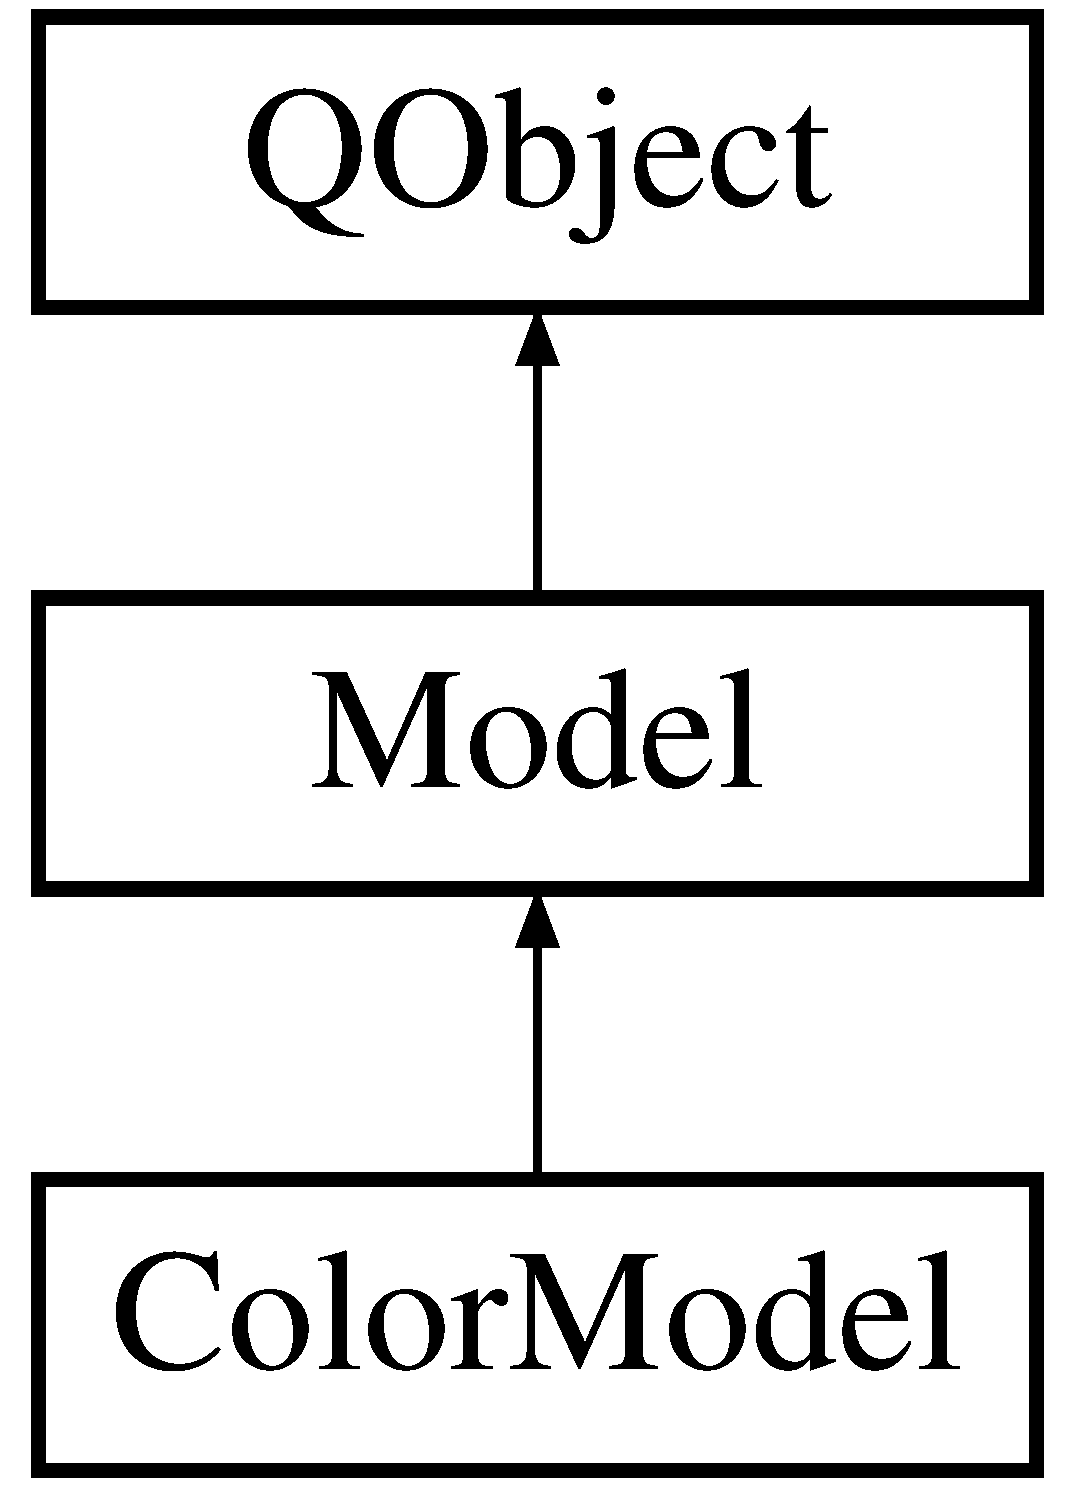
\includegraphics[height=3.000000cm]{class_color_model}
\end{center}
\end{figure}
\subsection*{Public Slots}
\begin{DoxyCompactItemize}
\item 
void \hyperlink{class_color_model_a747a1c9db1fb6f8eecf3a89adf5d5d37}{set\+Left\+Type} (Q\+String type)
\begin{DoxyCompactList}\small\item\em \hyperlink{class_color_model_a747a1c9db1fb6f8eecf3a89adf5d5d37}{Color\+Model\+::set\+Left\+Type}. \end{DoxyCompactList}\item 
void \hyperlink{class_color_model_a7954f6e500e4a2a7d9aa5813f5e288d5}{set\+Left\+Values} (Q\+Vector$<$ Q\+String $>$ values)
\begin{DoxyCompactList}\small\item\em \hyperlink{class_color_model_a7954f6e500e4a2a7d9aa5813f5e288d5}{Color\+Model\+::set\+Left\+Values}. \end{DoxyCompactList}\item 
void \hyperlink{class_color_model_acad4c21bc8bcede62c821f6e87a44e38}{set\+Right\+Type} (Q\+String type)
\begin{DoxyCompactList}\small\item\em \hyperlink{class_color_model_acad4c21bc8bcede62c821f6e87a44e38}{Color\+Model\+::set\+Right\+Type}. \end{DoxyCompactList}\item 
void \hyperlink{class_color_model_a07658db30b08f31f8f8190b6f4ed98d6}{set\+Right\+Values} (Q\+Vector$<$ Q\+String $>$ values)
\begin{DoxyCompactList}\small\item\em \hyperlink{class_color_model_a07658db30b08f31f8f8190b6f4ed98d6}{Color\+Model\+::set\+Right\+Values}. \end{DoxyCompactList}\item 
void \hyperlink{class_color_model_ae0c25592f1e201251a6090496548e762}{set\+Result\+Type} (Q\+String type)
\begin{DoxyCompactList}\small\item\em \hyperlink{class_color_model_ae0c25592f1e201251a6090496548e762}{Color\+Model\+::set\+Result\+Type} set the result type. \end{DoxyCompactList}\item 
void \hyperlink{class_color_model_ad51072410fbe8572066b3a53ca85a289}{set\+Op} (Q\+String e\+Operation)
\begin{DoxyCompactList}\small\item\em \hyperlink{class_color_model_ad51072410fbe8572066b3a53ca85a289}{Color\+Model\+::set\+Op}. \end{DoxyCompactList}\item 
\mbox{\Hypertarget{class_color_model_a3fcb0b558eb03b628a898f845dcb8640}\label{class_color_model_a3fcb0b558eb03b628a898f845dcb8640}} 
void \hyperlink{class_color_model_a3fcb0b558eb03b628a898f845dcb8640}{execute} ()
\begin{DoxyCompactList}\small\item\em \hyperlink{class_color_model_a3fcb0b558eb03b628a898f845dcb8640}{Color\+Model\+::execute} execute the operation. \end{DoxyCompactList}\item 
\mbox{\Hypertarget{class_color_model_ab64c059ce583856ec5dd9e35244ac92d}\label{class_color_model_ab64c059ce583856ec5dd9e35244ac92d}} 
void \hyperlink{class_color_model_ab64c059ce583856ec5dd9e35244ac92d}{get\+Result} ()
\begin{DoxyCompactList}\small\item\em \hyperlink{class_color_model_ab64c059ce583856ec5dd9e35244ac92d}{Color\+Model\+::get\+Result} set up result object. \end{DoxyCompactList}\item 
void \hyperlink{class_color_model_a90bcf6ca5b8d00a14a8153970594de97}{get\+History} ()
\begin{DoxyCompactList}\small\item\em \hyperlink{class_color_model_a90bcf6ca5b8d00a14a8153970594de97}{Color\+Model\+::get\+History}. \end{DoxyCompactList}\item 
\mbox{\Hypertarget{class_color_model_af5f09a79d9964daefb3ceac9c45f0034}\label{class_color_model_af5f09a79d9964daefb3ceac9c45f0034}} 
void \hyperlink{class_color_model_af5f09a79d9964daefb3ceac9c45f0034}{reset} ()
\begin{DoxyCompactList}\small\item\em \hyperlink{class_color_model_af5f09a79d9964daefb3ceac9c45f0034}{Color\+Model\+::reset} resets the \hyperlink{class_color_model}{Color\+Model} instance objects. \end{DoxyCompactList}\end{DoxyCompactItemize}
\subsection*{Public Member Functions}
\begin{DoxyCompactItemize}
\item 
\hyperlink{class_color_model_a2c2ee4adfbff8d5d5c9f7dc6fb7e9f3f}{Color\+Model} ()
\begin{DoxyCompactList}\small\item\em Model\+::\+Model inizialize the \hyperlink{class_color_model}{Color\+Model} and assign the older \hyperlink{class_color_model}{Color\+Model} if exists. \end{DoxyCompactList}\item 
\mbox{\Hypertarget{class_color_model_ace1f2efdd5fd223daa7e9cf002556a04}\label{class_color_model_ace1f2efdd5fd223daa7e9cf002556a04}} 
\hyperlink{class_color_model_ace1f2efdd5fd223daa7e9cf002556a04}{$\sim$\+Color\+Model} ()
\begin{DoxyCompactList}\small\item\em \hyperlink{class_color_model_ace1f2efdd5fd223daa7e9cf002556a04}{Color\+Model\+::$\sim$\+Color\+Model} deletes all \hyperlink{class_color}{Color} that \hyperlink{class_color_model}{Color\+Model} points to. \end{DoxyCompactList}\item 
Q\+Vector$<$ Q\+String $>$ \hyperlink{class_color_model_aab6a725338946ecec218220f5606be45}{available\+Operations} () const
\begin{DoxyCompactList}\small\item\em \hyperlink{class_color_model_aab6a725338946ecec218220f5606be45}{Color\+Model\+::available\+Operations}. \end{DoxyCompactList}\item 
Q\+Vector$<$ Q\+String $>$ \hyperlink{class_color_model_ac1788de4bf589070a2e915ff43d073ad}{all\+Available\+Types} () const
\begin{DoxyCompactList}\small\item\em \hyperlink{class_color_model_ac1788de4bf589070a2e915ff43d073ad}{Color\+Model\+::all\+Available\+Types}. \end{DoxyCompactList}\end{DoxyCompactItemize}
\subsection*{Additional Inherited Members}


\subsection{Detailed Description}
\hyperlink{class_color_model}{Color\+Model} implements the class \hyperlink{class_model}{Model} in the context of color representation. 

\subsection{Constructor \& Destructor Documentation}
\mbox{\Hypertarget{class_color_model_a2c2ee4adfbff8d5d5c9f7dc6fb7e9f3f}\label{class_color_model_a2c2ee4adfbff8d5d5c9f7dc6fb7e9f3f}} 
\index{Color\+Model@{Color\+Model}!Color\+Model@{Color\+Model}}
\index{Color\+Model@{Color\+Model}!Color\+Model@{Color\+Model}}
\subsubsection{\texorpdfstring{Color\+Model()}{ColorModel()}}
{\footnotesize\ttfamily Color\+Model\+::\+Color\+Model (\begin{DoxyParamCaption}{ }\end{DoxyParamCaption})}



Model\+::\+Model inizialize the \hyperlink{class_color_model}{Color\+Model} and assign the older \hyperlink{class_color_model}{Color\+Model} if exists. 


\begin{DoxyParams}{Parameters}
{\em previous} & \\
\hline
\end{DoxyParams}


\subsection{Member Function Documentation}
\mbox{\Hypertarget{class_color_model_ac1788de4bf589070a2e915ff43d073ad}\label{class_color_model_ac1788de4bf589070a2e915ff43d073ad}} 
\index{Color\+Model@{Color\+Model}!all\+Available\+Types@{all\+Available\+Types}}
\index{all\+Available\+Types@{all\+Available\+Types}!Color\+Model@{Color\+Model}}
\subsubsection{\texorpdfstring{all\+Available\+Types()}{allAvailableTypes()}}
{\footnotesize\ttfamily Q\+Vector$<$ Q\+String $>$ Color\+Model\+::all\+Available\+Types (\begin{DoxyParamCaption}{ }\end{DoxyParamCaption}) const\hspace{0.3cm}{\ttfamily [virtual]}}



\hyperlink{class_color_model_ac1788de4bf589070a2e915ff43d073ad}{Color\+Model\+::all\+Available\+Types}. 

\begin{DoxyReturn}{Returns}
Q\+Vector$<$\+Q\+String$>$ that contains all permitted types 
\end{DoxyReturn}


Implements \hyperlink{class_model}{Model}.

\mbox{\Hypertarget{class_color_model_aab6a725338946ecec218220f5606be45}\label{class_color_model_aab6a725338946ecec218220f5606be45}} 
\index{Color\+Model@{Color\+Model}!available\+Operations@{available\+Operations}}
\index{available\+Operations@{available\+Operations}!Color\+Model@{Color\+Model}}
\subsubsection{\texorpdfstring{available\+Operations()}{availableOperations()}}
{\footnotesize\ttfamily Q\+Vector$<$ Q\+String $>$ Color\+Model\+::available\+Operations (\begin{DoxyParamCaption}{ }\end{DoxyParamCaption}) const\hspace{0.3cm}{\ttfamily [virtual]}}



\hyperlink{class_color_model_aab6a725338946ecec218220f5606be45}{Color\+Model\+::available\+Operations}. 

\begin{DoxyReturn}{Returns}
Q\+Vector$<$\+Q\+String$>$ that contains all the operation that are available 
\end{DoxyReturn}


Implements \hyperlink{class_model}{Model}.

\mbox{\Hypertarget{class_color_model_a90bcf6ca5b8d00a14a8153970594de97}\label{class_color_model_a90bcf6ca5b8d00a14a8153970594de97}} 
\index{Color\+Model@{Color\+Model}!get\+History@{get\+History}}
\index{get\+History@{get\+History}!Color\+Model@{Color\+Model}}
\subsubsection{\texorpdfstring{get\+History}{getHistory}}
{\footnotesize\ttfamily void Color\+Model\+::get\+History (\begin{DoxyParamCaption}{ }\end{DoxyParamCaption})\hspace{0.3cm}{\ttfamily [slot]}}



\hyperlink{class_color_model_a90bcf6ca5b8d00a14a8153970594de97}{Color\+Model\+::get\+History}. 

\begin{DoxyReturn}{Returns}
Q\+Vector$<$\+Q\+String$>$ with the history of the operation that has been done 
\end{DoxyReturn}
\mbox{\Hypertarget{class_color_model_a747a1c9db1fb6f8eecf3a89adf5d5d37}\label{class_color_model_a747a1c9db1fb6f8eecf3a89adf5d5d37}} 
\index{Color\+Model@{Color\+Model}!set\+Left\+Type@{set\+Left\+Type}}
\index{set\+Left\+Type@{set\+Left\+Type}!Color\+Model@{Color\+Model}}
\subsubsection{\texorpdfstring{set\+Left\+Type}{setLeftType}}
{\footnotesize\ttfamily void Color\+Model\+::set\+Left\+Type (\begin{DoxyParamCaption}\item[{Q\+String}]{type }\end{DoxyParamCaption})\hspace{0.3cm}{\ttfamily [slot]}}



\hyperlink{class_color_model_a747a1c9db1fb6f8eecf3a89adf5d5d37}{Color\+Model\+::set\+Left\+Type}. 


\begin{DoxyParams}{Parameters}
{\em type} & setup the left operand type \\
\hline
\end{DoxyParams}
\mbox{\Hypertarget{class_color_model_a7954f6e500e4a2a7d9aa5813f5e288d5}\label{class_color_model_a7954f6e500e4a2a7d9aa5813f5e288d5}} 
\index{Color\+Model@{Color\+Model}!set\+Left\+Values@{set\+Left\+Values}}
\index{set\+Left\+Values@{set\+Left\+Values}!Color\+Model@{Color\+Model}}
\subsubsection{\texorpdfstring{set\+Left\+Values}{setLeftValues}}
{\footnotesize\ttfamily void Color\+Model\+::set\+Left\+Values (\begin{DoxyParamCaption}\item[{Q\+Vector$<$ Q\+String $>$}]{values }\end{DoxyParamCaption})\hspace{0.3cm}{\ttfamily [slot]}}



\hyperlink{class_color_model_a7954f6e500e4a2a7d9aa5813f5e288d5}{Color\+Model\+::set\+Left\+Values}. 


\begin{DoxyParams}{Parameters}
{\em values} & set values to the left operand \\
\hline
\end{DoxyParams}
\mbox{\Hypertarget{class_color_model_ad51072410fbe8572066b3a53ca85a289}\label{class_color_model_ad51072410fbe8572066b3a53ca85a289}} 
\index{Color\+Model@{Color\+Model}!set\+Op@{set\+Op}}
\index{set\+Op@{set\+Op}!Color\+Model@{Color\+Model}}
\subsubsection{\texorpdfstring{set\+Op}{setOp}}
{\footnotesize\ttfamily void Color\+Model\+::set\+Op (\begin{DoxyParamCaption}\item[{Q\+String}]{e\+Operation }\end{DoxyParamCaption})\hspace{0.3cm}{\ttfamily [slot]}}



\hyperlink{class_color_model_ad51072410fbe8572066b3a53ca85a289}{Color\+Model\+::set\+Op}. 


\begin{DoxyParams}{Parameters}
{\em e\+Operation} & set up the operation that will be executed \\
\hline
\end{DoxyParams}
\mbox{\Hypertarget{class_color_model_ae0c25592f1e201251a6090496548e762}\label{class_color_model_ae0c25592f1e201251a6090496548e762}} 
\index{Color\+Model@{Color\+Model}!set\+Result\+Type@{set\+Result\+Type}}
\index{set\+Result\+Type@{set\+Result\+Type}!Color\+Model@{Color\+Model}}
\subsubsection{\texorpdfstring{set\+Result\+Type}{setResultType}}
{\footnotesize\ttfamily void Color\+Model\+::set\+Result\+Type (\begin{DoxyParamCaption}\item[{Q\+String}]{type }\end{DoxyParamCaption})\hspace{0.3cm}{\ttfamily [slot]}}



\hyperlink{class_color_model_ae0c25592f1e201251a6090496548e762}{Color\+Model\+::set\+Result\+Type} set the result type. 


\begin{DoxyParams}{Parameters}
{\em type} & \\
\hline
\end{DoxyParams}
\mbox{\Hypertarget{class_color_model_acad4c21bc8bcede62c821f6e87a44e38}\label{class_color_model_acad4c21bc8bcede62c821f6e87a44e38}} 
\index{Color\+Model@{Color\+Model}!set\+Right\+Type@{set\+Right\+Type}}
\index{set\+Right\+Type@{set\+Right\+Type}!Color\+Model@{Color\+Model}}
\subsubsection{\texorpdfstring{set\+Right\+Type}{setRightType}}
{\footnotesize\ttfamily void Color\+Model\+::set\+Right\+Type (\begin{DoxyParamCaption}\item[{Q\+String}]{type }\end{DoxyParamCaption})\hspace{0.3cm}{\ttfamily [slot]}}



\hyperlink{class_color_model_acad4c21bc8bcede62c821f6e87a44e38}{Color\+Model\+::set\+Right\+Type}. 


\begin{DoxyParams}{Parameters}
{\em type} & set the right operand type \\
\hline
\end{DoxyParams}
\mbox{\Hypertarget{class_color_model_a07658db30b08f31f8f8190b6f4ed98d6}\label{class_color_model_a07658db30b08f31f8f8190b6f4ed98d6}} 
\index{Color\+Model@{Color\+Model}!set\+Right\+Values@{set\+Right\+Values}}
\index{set\+Right\+Values@{set\+Right\+Values}!Color\+Model@{Color\+Model}}
\subsubsection{\texorpdfstring{set\+Right\+Values}{setRightValues}}
{\footnotesize\ttfamily void Color\+Model\+::set\+Right\+Values (\begin{DoxyParamCaption}\item[{Q\+Vector$<$ Q\+String $>$}]{values }\end{DoxyParamCaption})\hspace{0.3cm}{\ttfamily [slot]}}



\hyperlink{class_color_model_a07658db30b08f31f8f8190b6f4ed98d6}{Color\+Model\+::set\+Right\+Values}. 


\begin{DoxyParams}{Parameters}
{\em values} & set values to the right operand \\
\hline
\end{DoxyParams}


The documentation for this class was generated from the following files\+:\begin{DoxyCompactItemize}
\item 
/home/gian/\+Projects/\+Kalk2-\/0/\+Kalk/\+Model/\hyperlink{colormodel_8h}{colormodel.\+h}\item 
/home/gian/\+Projects/\+Kalk2-\/0/\+Kalk/\+Model/colormodel.\+cpp\end{DoxyCompactItemize}

\hypertarget{class_console_view}{}\section{Console\+View Class Reference}
\label{class_console_view}\index{Console\+View@{Console\+View}}


\hyperlink{class_console_view}{Console\+View} exestends the \hyperlink{class_view}{View} class Console provides an interface in terminal line.  




{\ttfamily \#include $<$consoleview.\+h$>$}

Inheritance diagram for Console\+View\+:\begin{figure}[H]
\begin{center}
\leavevmode
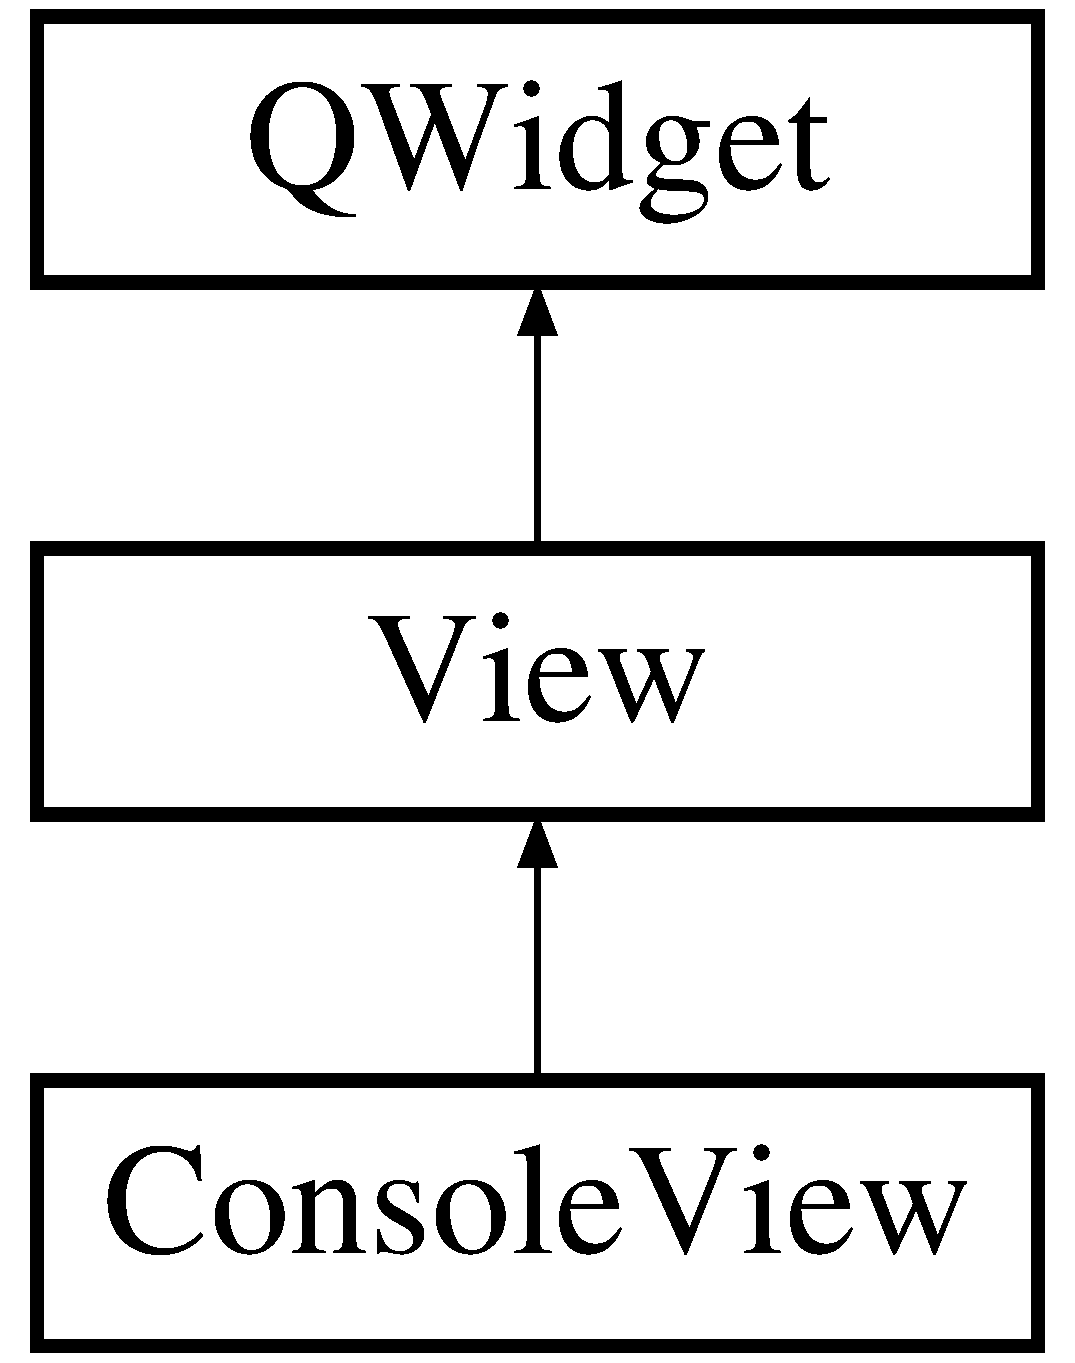
\includegraphics[height=3.000000cm]{class_console_view}
\end{center}
\end{figure}
\subsection*{Public Slots}
\begin{DoxyCompactItemize}
\item 
void \hyperlink{class_console_view_a6d88d3e3957fb1cdea6e076770fffdec}{set\+Available\+Operations} (const Q\+Vector$<$ Q\+String $>$ operations)
\begin{DoxyCompactList}\small\item\em \hyperlink{class_console_view_a6d88d3e3957fb1cdea6e076770fffdec}{Console\+View\+::set\+Available\+Operations}. \end{DoxyCompactList}\item 
void \hyperlink{class_console_view_a17864810f831eb58d8be275a2eaa461d}{set\+Permitted\+Operations} (const Q\+Vector$<$ Q\+String $>$ operations)
\begin{DoxyCompactList}\small\item\em \hyperlink{class_console_view_a17864810f831eb58d8be275a2eaa461d}{Console\+View\+::set\+Permitted\+Operations}. \end{DoxyCompactList}\item 
void \hyperlink{class_console_view_a7dcc84dc917fb81babae471315e9cefd}{set\+Left\+Types} (const Q\+Vector$<$ Q\+String $>$ types)
\begin{DoxyCompactList}\small\item\em \hyperlink{class_console_view_a7dcc84dc917fb81babae471315e9cefd}{Console\+View\+::set\+Left\+Types}. \end{DoxyCompactList}\item 
void \hyperlink{class_console_view_ae813b6a54bc56f1a22b60ee005da813e}{set\+Left\+Fields} (const int \&fields, const Q\+Vector$<$ Q\+String $>$ \&limits)
\begin{DoxyCompactList}\small\item\em \hyperlink{class_console_view_ae813b6a54bc56f1a22b60ee005da813e}{Console\+View\+::set\+Left\+Fields}. \end{DoxyCompactList}\item 
void \hyperlink{class_console_view_a96f03ac06e40ae1d45601ac9f11863c4}{set\+Right\+Types} (const Q\+Vector$<$ Q\+String $>$ types)
\begin{DoxyCompactList}\small\item\em \hyperlink{class_console_view_a96f03ac06e40ae1d45601ac9f11863c4}{Console\+View\+::set\+Right\+Types}. \end{DoxyCompactList}\item 
void \hyperlink{class_console_view_a2b9ba00770ebdeda35f2b506c752248e}{set\+Right\+Fields} (const int \&fields, const Q\+Vector$<$ Q\+String $>$ \&limits)
\begin{DoxyCompactList}\small\item\em \hyperlink{class_console_view_a2b9ba00770ebdeda35f2b506c752248e}{Console\+View\+::set\+Right\+Fields}. \end{DoxyCompactList}\item 
void \hyperlink{class_console_view_a0b43a9e8d693b227fcd3a00b7a384e37}{set\+Result} (const Q\+Vector$<$ Q\+String $>$ result)
\begin{DoxyCompactList}\small\item\em \hyperlink{class_console_view_a0b43a9e8d693b227fcd3a00b7a384e37}{Console\+View\+::set\+Result}. \end{DoxyCompactList}\item 
void \hyperlink{class_console_view_afeb190605800a7ce7b8b3224a32b15a3}{set\+Result\+Fields} (const int \&fields)
\begin{DoxyCompactList}\small\item\em \hyperlink{class_console_view_afeb190605800a7ce7b8b3224a32b15a3}{Console\+View\+::set\+Result\+Fields}. \end{DoxyCompactList}\item 
void \hyperlink{class_console_view_acd2e5ae5d77096c4227c2c9c5881926b}{set\+History} (const Q\+Vector$<$ Q\+Vector$<$ Q\+String $>$$>$ \&history)
\begin{DoxyCompactList}\small\item\em \hyperlink{class_console_view_acd2e5ae5d77096c4227c2c9c5881926b}{Console\+View\+::set\+History}. \end{DoxyCompactList}\item 
void \hyperlink{class_console_view_a3c5b8df5fd316a1190f7beaa0460b29a}{error} (const Q\+String \&error\+\_\+message)
\begin{DoxyCompactList}\small\item\em \hyperlink{class_console_view_a3c5b8df5fd316a1190f7beaa0460b29a}{Console\+View\+::error} prints error message in terminal. \end{DoxyCompactList}\item 
void \hyperlink{class_console_view_aba1141da17dd4f424ae296142ff7a8bd}{reset\+Type} (Q\+String drop, Q\+String type)
\begin{DoxyCompactList}\small\item\em \hyperlink{class_console_view_aba1141da17dd4f424ae296142ff7a8bd}{Console\+View\+::reset\+Type}. \end{DoxyCompactList}\item 
\mbox{\Hypertarget{class_console_view_a64444203b69213adbe63da93d3d03cb4}\label{class_console_view_a64444203b69213adbe63da93d3d03cb4}} 
void \hyperlink{class_console_view_a64444203b69213adbe63da93d3d03cb4}{show} ()
\begin{DoxyCompactList}\small\item\em \hyperlink{class_console_view_a64444203b69213adbe63da93d3d03cb4}{Console\+View\+::show} inizialize the view inside the terminal. \end{DoxyCompactList}\end{DoxyCompactItemize}
\subsection*{Public Member Functions}
\begin{DoxyCompactItemize}
\item 
\mbox{\Hypertarget{class_console_view_ae8a2079a84bc7b7e2b8a68f927cae911}\label{class_console_view_ae8a2079a84bc7b7e2b8a68f927cae911}} 
{\bfseries Console\+View} (\hyperlink{class_view}{View} $\ast$parent=nullptr)
\item 
\hyperlink{class_console_view_a42ca0ca912c42d743a64f7e3a80b6f26}{Console\+View} (const \hyperlink{class_console_view}{Console\+View} \&console)
\begin{DoxyCompactList}\small\item\em Console\+View\+::\+Console\+View. \end{DoxyCompactList}\end{DoxyCompactItemize}
\subsection*{Additional Inherited Members}


\subsection{Detailed Description}
\hyperlink{class_console_view}{Console\+View} exestends the \hyperlink{class_view}{View} class Console provides an interface in terminal line. 

\subsection{Constructor \& Destructor Documentation}
\mbox{\Hypertarget{class_console_view_a42ca0ca912c42d743a64f7e3a80b6f26}\label{class_console_view_a42ca0ca912c42d743a64f7e3a80b6f26}} 
\index{Console\+View@{Console\+View}!Console\+View@{Console\+View}}
\index{Console\+View@{Console\+View}!Console\+View@{Console\+View}}
\subsubsection{\texorpdfstring{Console\+View()}{ConsoleView()}}
{\footnotesize\ttfamily Console\+View\+::\+Console\+View (\begin{DoxyParamCaption}\item[{const \hyperlink{class_console_view}{Console\+View} \&}]{console }\end{DoxyParamCaption})}



Console\+View\+::\+Console\+View. 


\begin{DoxyParams}{Parameters}
{\em console} & \\
\hline
\end{DoxyParams}


\subsection{Member Function Documentation}
\mbox{\Hypertarget{class_console_view_a3c5b8df5fd316a1190f7beaa0460b29a}\label{class_console_view_a3c5b8df5fd316a1190f7beaa0460b29a}} 
\index{Console\+View@{Console\+View}!error@{error}}
\index{error@{error}!Console\+View@{Console\+View}}
\subsubsection{\texorpdfstring{error}{error}}
{\footnotesize\ttfamily void Console\+View\+::error (\begin{DoxyParamCaption}\item[{const Q\+String \&}]{error\+\_\+message }\end{DoxyParamCaption})\hspace{0.3cm}{\ttfamily [slot]}}



\hyperlink{class_console_view_a3c5b8df5fd316a1190f7beaa0460b29a}{Console\+View\+::error} prints error message in terminal. 


\begin{DoxyParams}{Parameters}
{\em error\+\_\+message} & \\
\hline
\end{DoxyParams}
\mbox{\Hypertarget{class_console_view_aba1141da17dd4f424ae296142ff7a8bd}\label{class_console_view_aba1141da17dd4f424ae296142ff7a8bd}} 
\index{Console\+View@{Console\+View}!reset\+Type@{reset\+Type}}
\index{reset\+Type@{reset\+Type}!Console\+View@{Console\+View}}
\subsubsection{\texorpdfstring{reset\+Type}{resetType}}
{\footnotesize\ttfamily void Console\+View\+::reset\+Type (\begin{DoxyParamCaption}\item[{Q\+String}]{drop,  }\item[{Q\+String}]{type }\end{DoxyParamCaption})\hspace{0.3cm}{\ttfamily [slot]}}



\hyperlink{class_console_view_aba1141da17dd4f424ae296142ff7a8bd}{Console\+View\+::reset\+Type}. 


\begin{DoxyParams}{Parameters}
{\em drop} & \\
\hline
{\em type} & \\
\hline
\end{DoxyParams}
\mbox{\Hypertarget{class_console_view_a6d88d3e3957fb1cdea6e076770fffdec}\label{class_console_view_a6d88d3e3957fb1cdea6e076770fffdec}} 
\index{Console\+View@{Console\+View}!set\+Available\+Operations@{set\+Available\+Operations}}
\index{set\+Available\+Operations@{set\+Available\+Operations}!Console\+View@{Console\+View}}
\subsubsection{\texorpdfstring{set\+Available\+Operations}{setAvailableOperations}}
{\footnotesize\ttfamily void Console\+View\+::set\+Available\+Operations (\begin{DoxyParamCaption}\item[{const Q\+Vector$<$ Q\+String $>$}]{operations }\end{DoxyParamCaption})\hspace{0.3cm}{\ttfamily [slot]}}



\hyperlink{class_console_view_a6d88d3e3957fb1cdea6e076770fffdec}{Console\+View\+::set\+Available\+Operations}. 


\begin{DoxyParams}{Parameters}
{\em opt} & sets up all operations that are available not really required \\
\hline
\end{DoxyParams}
\mbox{\Hypertarget{class_console_view_acd2e5ae5d77096c4227c2c9c5881926b}\label{class_console_view_acd2e5ae5d77096c4227c2c9c5881926b}} 
\index{Console\+View@{Console\+View}!set\+History@{set\+History}}
\index{set\+History@{set\+History}!Console\+View@{Console\+View}}
\subsubsection{\texorpdfstring{set\+History}{setHistory}}
{\footnotesize\ttfamily void Console\+View\+::set\+History (\begin{DoxyParamCaption}\item[{const Q\+Vector$<$ Q\+Vector$<$ Q\+String $>$$>$ \&}]{history }\end{DoxyParamCaption})\hspace{0.3cm}{\ttfamily [slot]}}



\hyperlink{class_console_view_acd2e5ae5d77096c4227c2c9c5881926b}{Console\+View\+::set\+History}. 


\begin{DoxyParams}{Parameters}
{\em history} & shows history on terminal \\
\hline
\end{DoxyParams}
\mbox{\Hypertarget{class_console_view_ae813b6a54bc56f1a22b60ee005da813e}\label{class_console_view_ae813b6a54bc56f1a22b60ee005da813e}} 
\index{Console\+View@{Console\+View}!set\+Left\+Fields@{set\+Left\+Fields}}
\index{set\+Left\+Fields@{set\+Left\+Fields}!Console\+View@{Console\+View}}
\subsubsection{\texorpdfstring{set\+Left\+Fields}{setLeftFields}}
{\footnotesize\ttfamily void Console\+View\+::set\+Left\+Fields (\begin{DoxyParamCaption}\item[{const int \&}]{fields,  }\item[{const Q\+Vector$<$ Q\+String $>$ \&}]{limits }\end{DoxyParamCaption})\hspace{0.3cm}{\ttfamily [slot]}}



\hyperlink{class_console_view_ae813b6a54bc56f1a22b60ee005da813e}{Console\+View\+::set\+Left\+Fields}. 


\begin{DoxyParams}{Parameters}
{\em fields} & sets up l\+\_\+size variable \\
\hline
\end{DoxyParams}
\mbox{\Hypertarget{class_console_view_a7dcc84dc917fb81babae471315e9cefd}\label{class_console_view_a7dcc84dc917fb81babae471315e9cefd}} 
\index{Console\+View@{Console\+View}!set\+Left\+Types@{set\+Left\+Types}}
\index{set\+Left\+Types@{set\+Left\+Types}!Console\+View@{Console\+View}}
\subsubsection{\texorpdfstring{set\+Left\+Types}{setLeftTypes}}
{\footnotesize\ttfamily void Console\+View\+::set\+Left\+Types (\begin{DoxyParamCaption}\item[{const Q\+Vector$<$ Q\+String $>$}]{types }\end{DoxyParamCaption})\hspace{0.3cm}{\ttfamily [slot]}}



\hyperlink{class_console_view_a7dcc84dc917fb81babae471315e9cefd}{Console\+View\+::set\+Left\+Types}. 


\begin{DoxyParams}{Parameters}
{\em types} & sets up l\+\_\+types variable \\
\hline
\end{DoxyParams}
\mbox{\Hypertarget{class_console_view_a17864810f831eb58d8be275a2eaa461d}\label{class_console_view_a17864810f831eb58d8be275a2eaa461d}} 
\index{Console\+View@{Console\+View}!set\+Permitted\+Operations@{set\+Permitted\+Operations}}
\index{set\+Permitted\+Operations@{set\+Permitted\+Operations}!Console\+View@{Console\+View}}
\subsubsection{\texorpdfstring{set\+Permitted\+Operations}{setPermittedOperations}}
{\footnotesize\ttfamily void Console\+View\+::set\+Permitted\+Operations (\begin{DoxyParamCaption}\item[{const Q\+Vector$<$ Q\+String $>$}]{operations }\end{DoxyParamCaption})\hspace{0.3cm}{\ttfamily [slot]}}



\hyperlink{class_console_view_a17864810f831eb58d8be275a2eaa461d}{Console\+View\+::set\+Permitted\+Operations}. 


\begin{DoxyParams}{Parameters}
{\em opt} & sets up all operations that the user can execute \\
\hline
\end{DoxyParams}
\mbox{\Hypertarget{class_console_view_a0b43a9e8d693b227fcd3a00b7a384e37}\label{class_console_view_a0b43a9e8d693b227fcd3a00b7a384e37}} 
\index{Console\+View@{Console\+View}!set\+Result@{set\+Result}}
\index{set\+Result@{set\+Result}!Console\+View@{Console\+View}}
\subsubsection{\texorpdfstring{set\+Result}{setResult}}
{\footnotesize\ttfamily void Console\+View\+::set\+Result (\begin{DoxyParamCaption}\item[{const Q\+Vector$<$ Q\+String $>$}]{result }\end{DoxyParamCaption})\hspace{0.3cm}{\ttfamily [slot]}}



\hyperlink{class_console_view_a0b43a9e8d693b227fcd3a00b7a384e37}{Console\+View\+::set\+Result}. 


\begin{DoxyParams}{Parameters}
{\em result} & sets up local\+\_\+result variable \\
\hline
\end{DoxyParams}
\mbox{\Hypertarget{class_console_view_afeb190605800a7ce7b8b3224a32b15a3}\label{class_console_view_afeb190605800a7ce7b8b3224a32b15a3}} 
\index{Console\+View@{Console\+View}!set\+Result\+Fields@{set\+Result\+Fields}}
\index{set\+Result\+Fields@{set\+Result\+Fields}!Console\+View@{Console\+View}}
\subsubsection{\texorpdfstring{set\+Result\+Fields}{setResultFields}}
{\footnotesize\ttfamily void Console\+View\+::set\+Result\+Fields (\begin{DoxyParamCaption}\item[{const int \&}]{fields }\end{DoxyParamCaption})\hspace{0.3cm}{\ttfamily [slot]}}



\hyperlink{class_console_view_afeb190605800a7ce7b8b3224a32b15a3}{Console\+View\+::set\+Result\+Fields}. 


\begin{DoxyParams}{Parameters}
{\em fields} & does nothing because the result\+Fields are the same as left operand \\
\hline
\end{DoxyParams}
\mbox{\Hypertarget{class_console_view_a2b9ba00770ebdeda35f2b506c752248e}\label{class_console_view_a2b9ba00770ebdeda35f2b506c752248e}} 
\index{Console\+View@{Console\+View}!set\+Right\+Fields@{set\+Right\+Fields}}
\index{set\+Right\+Fields@{set\+Right\+Fields}!Console\+View@{Console\+View}}
\subsubsection{\texorpdfstring{set\+Right\+Fields}{setRightFields}}
{\footnotesize\ttfamily void Console\+View\+::set\+Right\+Fields (\begin{DoxyParamCaption}\item[{const int \&}]{fields,  }\item[{const Q\+Vector$<$ Q\+String $>$ \&}]{limits }\end{DoxyParamCaption})\hspace{0.3cm}{\ttfamily [slot]}}



\hyperlink{class_console_view_a2b9ba00770ebdeda35f2b506c752248e}{Console\+View\+::set\+Right\+Fields}. 


\begin{DoxyParams}{Parameters}
{\em fields} & sets up r\+\_\+size variable \\
\hline
\end{DoxyParams}
\mbox{\Hypertarget{class_console_view_a96f03ac06e40ae1d45601ac9f11863c4}\label{class_console_view_a96f03ac06e40ae1d45601ac9f11863c4}} 
\index{Console\+View@{Console\+View}!set\+Right\+Types@{set\+Right\+Types}}
\index{set\+Right\+Types@{set\+Right\+Types}!Console\+View@{Console\+View}}
\subsubsection{\texorpdfstring{set\+Right\+Types}{setRightTypes}}
{\footnotesize\ttfamily void Console\+View\+::set\+Right\+Types (\begin{DoxyParamCaption}\item[{const Q\+Vector$<$ Q\+String $>$}]{types }\end{DoxyParamCaption})\hspace{0.3cm}{\ttfamily [slot]}}



\hyperlink{class_console_view_a96f03ac06e40ae1d45601ac9f11863c4}{Console\+View\+::set\+Right\+Types}. 


\begin{DoxyParams}{Parameters}
{\em types} & sets up r\+\_\+types variable \\
\hline
\end{DoxyParams}


The documentation for this class was generated from the following files\+:\begin{DoxyCompactItemize}
\item 
/home/gian/\+Projects/\+Kalk2-\/0/\+Kalk/\+View/\+Console/\hyperlink{consoleview_8h}{consoleview.\+h}\item 
/home/gian/\+Projects/\+Kalk2-\/0/\+Kalk/\+View/\+Console/consoleview.\+cpp\end{DoxyCompactItemize}

\hypertarget{class_controller}{}\section{Controller Class Reference}
\label{class_controller}\index{Controller@{Controller}}


this class handles the connection between model and view  




{\ttfamily \#include $<$controller.\+h$>$}

Inheritance diagram for Controller\+:\begin{figure}[H]
\begin{center}
\leavevmode
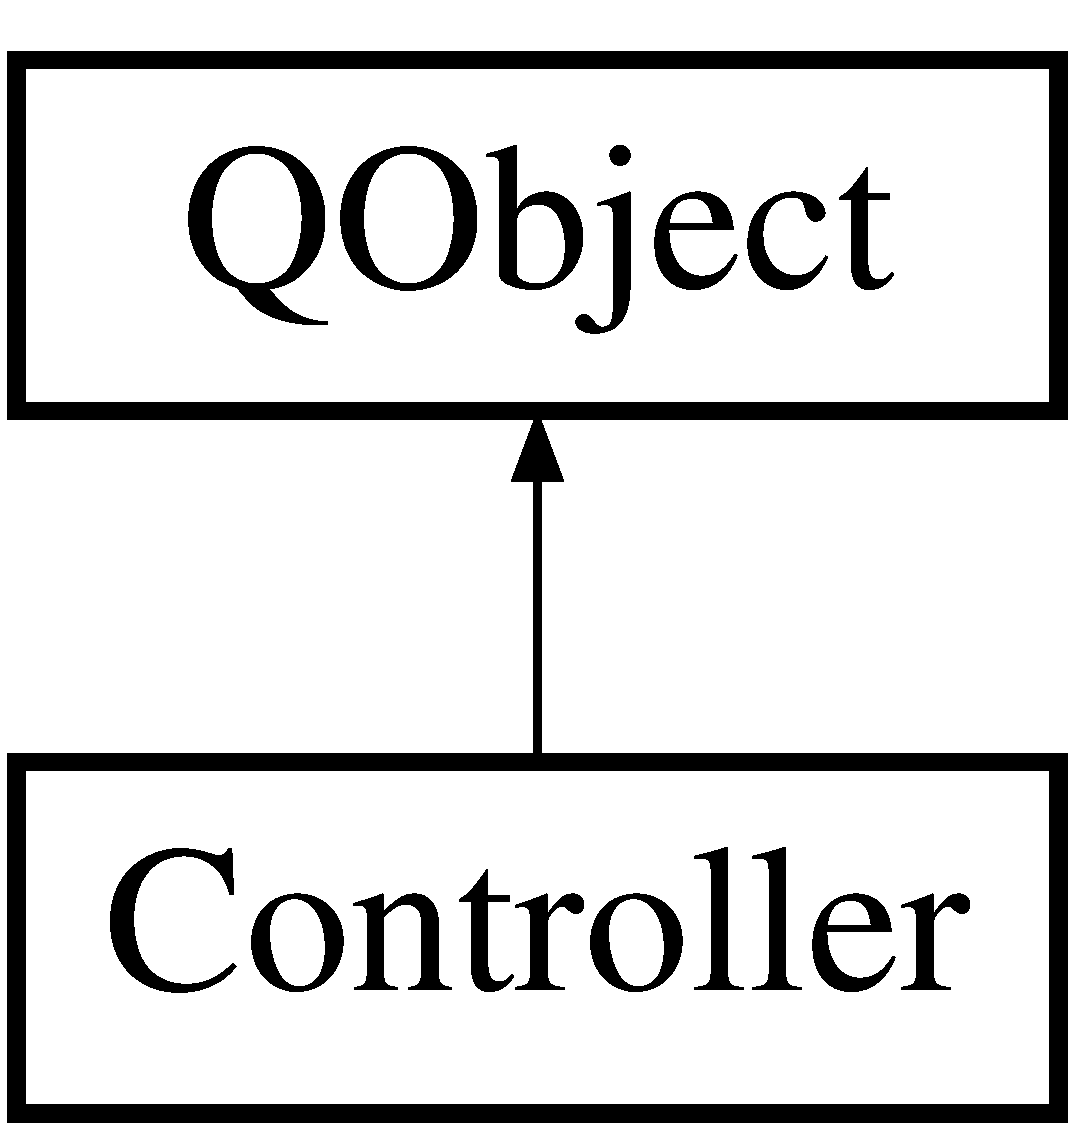
\includegraphics[height=2.000000cm]{class_controller}
\end{center}
\end{figure}
\subsection*{Public Slots}
\begin{DoxyCompactItemize}
\item 
\mbox{\Hypertarget{class_controller_ac5b5525e1a9fc6914657dd8d943a0928}\label{class_controller_ac5b5525e1a9fc6914657dd8d943a0928}} 
void \hyperlink{class_controller_ac5b5525e1a9fc6914657dd8d943a0928}{set\+Up} ()
\begin{DoxyCompactList}\small\item\em \hyperlink{class_controller_ac5b5525e1a9fc6914657dd8d943a0928}{Controller\+::set\+Up} set up the object view usign model information. \end{DoxyCompactList}\end{DoxyCompactItemize}
\subsection*{Public Member Functions}
\begin{DoxyCompactItemize}
\item 
\hyperlink{class_controller_a7984f40669752a82c87e067bec6c3751}{Controller} (\hyperlink{class_model}{Model} $\ast$f\+\_\+model, \hyperlink{class_view}{View} $\ast$f\+\_\+view)
\begin{DoxyCompactList}\small\item\em \hyperlink{class_controller_a7984f40669752a82c87e067bec6c3751}{Controller\+::\+Controller}. \end{DoxyCompactList}\item 
\mbox{\Hypertarget{class_controller_a0ab87934c4f7a266cfdb86e0f36bc1b5}\label{class_controller_a0ab87934c4f7a266cfdb86e0f36bc1b5}} 
\hyperlink{class_controller_a0ab87934c4f7a266cfdb86e0f36bc1b5}{$\sim$\+Controller} ()
\begin{DoxyCompactList}\small\item\em \hyperlink{class_controller_a0ab87934c4f7a266cfdb86e0f36bc1b5}{Controller\+::$\sim$\+Controller}. \end{DoxyCompactList}\item 
\mbox{\Hypertarget{class_controller_afe28638e4396e7b8415cbe5d05964ad2}\label{class_controller_afe28638e4396e7b8415cbe5d05964ad2}} 
void \hyperlink{class_controller_afe28638e4396e7b8415cbe5d05964ad2}{connect} ()
\begin{DoxyCompactList}\small\item\em \hyperlink{class_controller_afe28638e4396e7b8415cbe5d05964ad2}{Controller\+::connect} Connects all the slots and signal in view and model. \end{DoxyCompactList}\item 
\mbox{\Hypertarget{class_controller_a1b122dccfa346274aa2e6aa5e6a7eb01}\label{class_controller_a1b122dccfa346274aa2e6aa5e6a7eb01}} 
void \hyperlink{class_controller_a1b122dccfa346274aa2e6aa5e6a7eb01}{disconnect} ()
\begin{DoxyCompactList}\small\item\em \hyperlink{class_controller_a1b122dccfa346274aa2e6aa5e6a7eb01}{Controller\+::disconnect} disconnects all the slots and signal in view and model. \end{DoxyCompactList}\end{DoxyCompactItemize}


\subsection{Detailed Description}
this class handles the connection between model and view 

\begin{DoxyDate}{Date}
15/08/2018 
\end{DoxyDate}


\subsection{Constructor \& Destructor Documentation}
\mbox{\Hypertarget{class_controller_a7984f40669752a82c87e067bec6c3751}\label{class_controller_a7984f40669752a82c87e067bec6c3751}} 
\index{Controller@{Controller}!Controller@{Controller}}
\index{Controller@{Controller}!Controller@{Controller}}
\subsubsection{\texorpdfstring{Controller()}{Controller()}}
{\footnotesize\ttfamily Controller\+::\+Controller (\begin{DoxyParamCaption}\item[{\hyperlink{class_model}{Model} $\ast$}]{f\+\_\+model,  }\item[{\hyperlink{class_view}{View} $\ast$}]{f\+\_\+view }\end{DoxyParamCaption})}



\hyperlink{class_controller_a7984f40669752a82c87e067bec6c3751}{Controller\+::\+Controller}. 


\begin{DoxyParams}{Parameters}
{\em f\+\_\+model} & \\
\hline
{\em f\+\_\+view} & \\
\hline
\end{DoxyParams}


The documentation for this class was generated from the following files\+:\begin{DoxyCompactItemize}
\item 
/home/gian/\+Projects/\+Kalk2-\/0/\+Kalk/\+Controller/\hyperlink{controller_8h}{controller.\+h}\item 
/home/gian/\+Projects/\+Kalk2-\/0/\+Kalk/\+Controller/controller.\+cpp\end{DoxyCompactItemize}

\hypertarget{class_c_y_m_k}{}\section{C\+Y\+MK Class Reference}
\label{class_c_y_m_k}\index{C\+Y\+MK@{C\+Y\+MK}}


this class uses as base the class \hyperlink{class_c_i_exyz}{C\+I\+Exyz} \hyperlink{class_c_y_m_k}{C\+Y\+MK} stores a color in \hyperlink{class_c_y_m_k}{C\+Y\+MK} representation  




{\ttfamily \#include $<$cymk.\+h$>$}

Inheritance diagram for C\+Y\+MK\+:\begin{figure}[H]
\begin{center}
\leavevmode
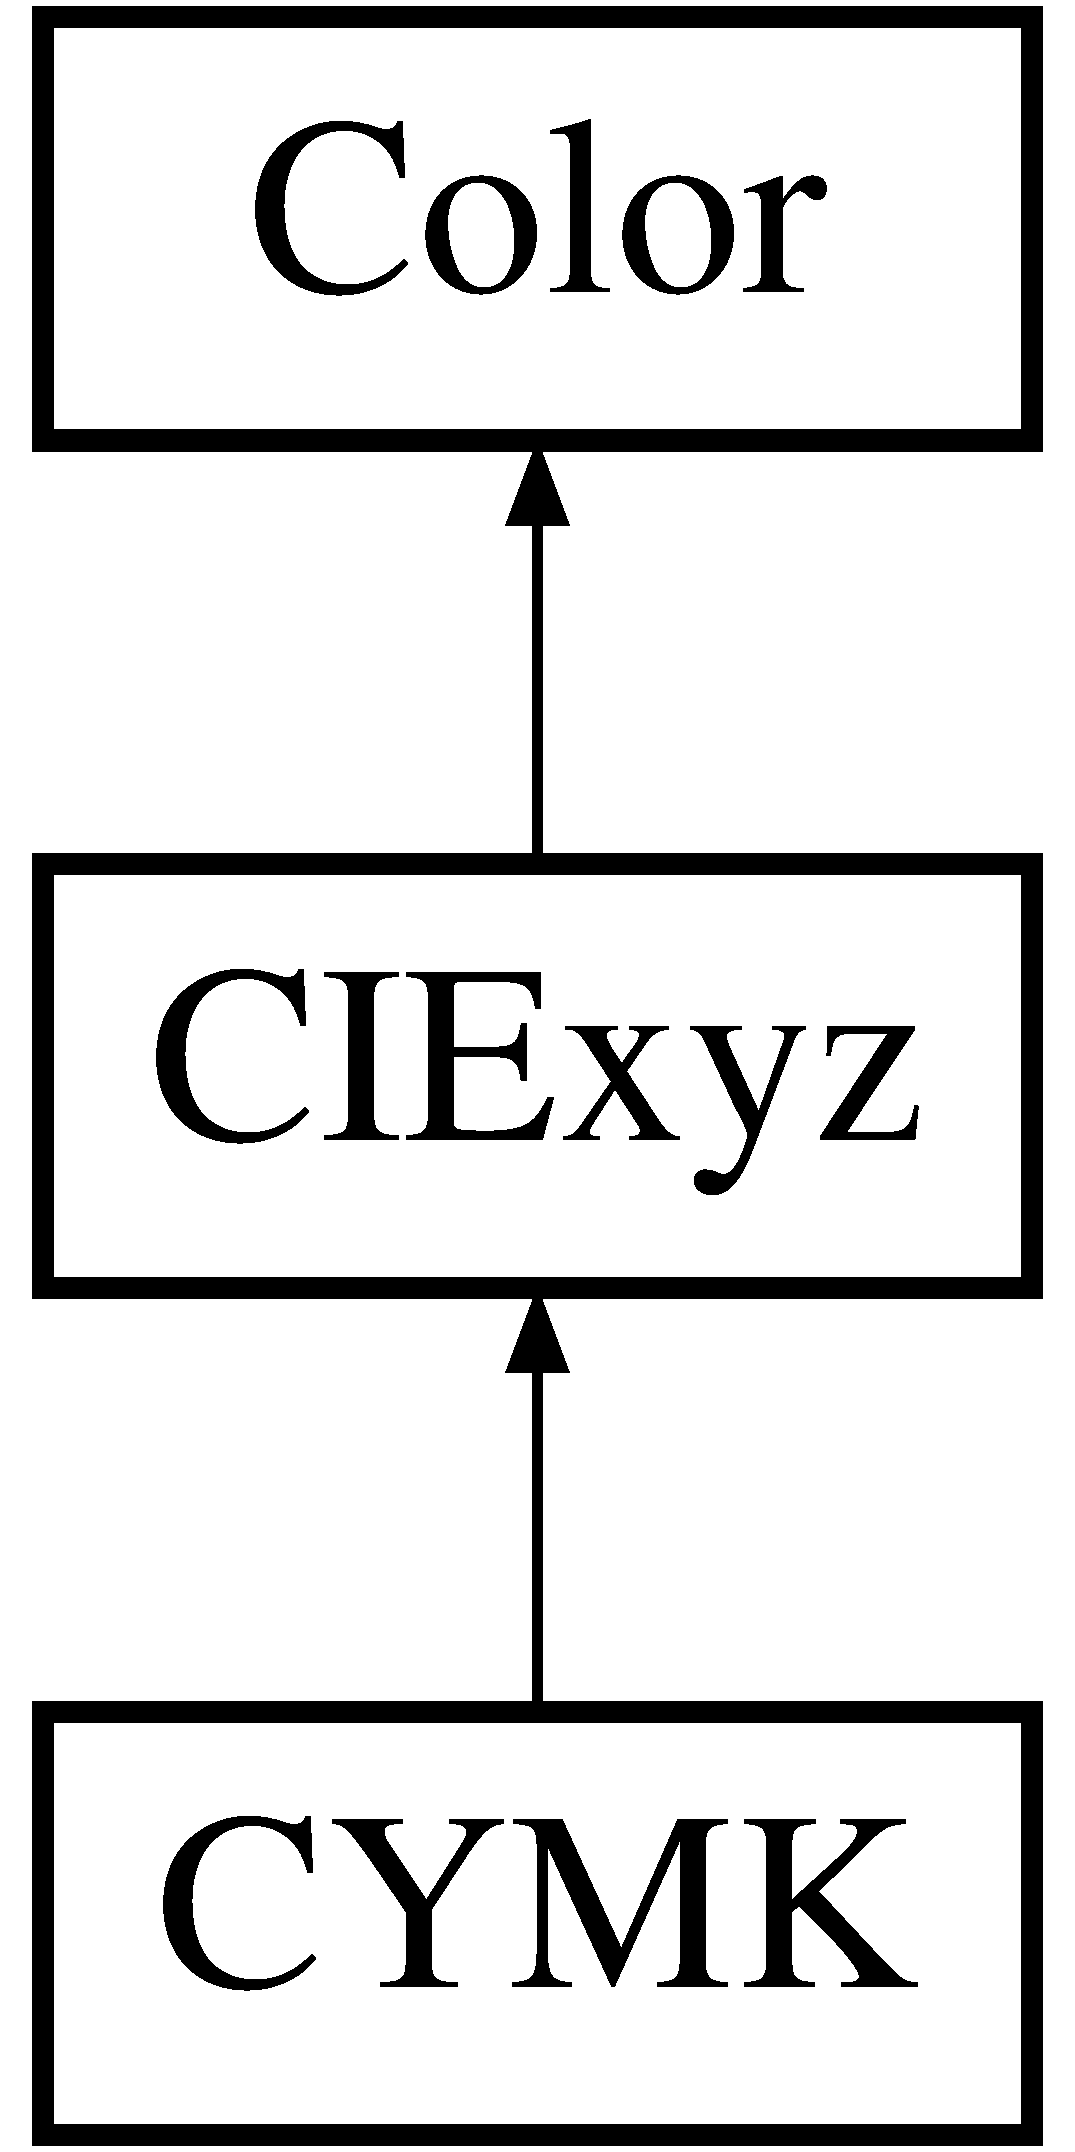
\includegraphics[height=3.000000cm]{class_c_y_m_k}
\end{center}
\end{figure}
\subsection*{Public Member Functions}
\begin{DoxyCompactItemize}
\item 
\hyperlink{class_c_y_m_k_a1aa6a0953837818a2b298476cab9388d}{C\+Y\+MK} (unsigned int c=0, unsigned int y=0, unsigned int m=0, unsigned int k=0)
\begin{DoxyCompactList}\small\item\em \hyperlink{class_c_y_m_k_a1aa6a0953837818a2b298476cab9388d}{C\+Y\+M\+K\+::\+C\+Y\+MK} Constructor for \hyperlink{class_c_y_m_k}{C\+Y\+MK} color representation from unsigned int numbers. \end{DoxyCompactList}\item 
\hyperlink{class_c_y_m_k_ab524ef2e847938b2efff28886387ec51}{C\+Y\+MK} (const \hyperlink{class_color}{Color} $\ast$from)
\begin{DoxyCompactList}\small\item\em \hyperlink{class_c_y_m_k_a1aa6a0953837818a2b298476cab9388d}{C\+Y\+M\+K\+::\+C\+Y\+MK} Constructor for \hyperlink{class_c_y_m_k}{C\+Y\+MK} color representation from \hyperlink{class_color}{Color} pointer. \end{DoxyCompactList}\item 
\hyperlink{class_c_y_m_k_a4bccfb3b46229aa82827bd6988efaa8c}{C\+Y\+MK} (const \hyperlink{class_c_y_m_k}{C\+Y\+MK} \&from)
\begin{DoxyCompactList}\small\item\em \hyperlink{class_c_y_m_k_a1aa6a0953837818a2b298476cab9388d}{C\+Y\+M\+K\+::\+C\+Y\+MK} copy constructor. \end{DoxyCompactList}\item 
Q\+String \hyperlink{class_c_y_m_k_aa523f734fd52f67ca9fcb31f0b7fe579}{get\+Representation} () const
\begin{DoxyCompactList}\small\item\em C\+Y\+M\+K\+::getrepresentation. \end{DoxyCompactList}\item 
\hyperlink{class_color}{Color} $\ast$ \hyperlink{class_c_y_m_k_a397c0109e76ff6cc331b49e4b73623ef}{negate} () const
\begin{DoxyCompactList}\small\item\em \hyperlink{class_c_y_m_k_a397c0109e76ff6cc331b49e4b73623ef}{C\+Y\+M\+K\+::negate}. \end{DoxyCompactList}\item 
\hyperlink{class_color}{Color} $\ast$ \hyperlink{class_c_y_m_k_adeb4691eafbb53e15538a3d829f59a14}{mix} (const \hyperlink{class_color}{Color} $\ast$a) const
\begin{DoxyCompactList}\small\item\em \hyperlink{class_c_y_m_k_adeb4691eafbb53e15538a3d829f59a14}{C\+Y\+M\+K\+::mix}. \end{DoxyCompactList}\item 
\hyperlink{class_color}{Color} $\ast$ \hyperlink{class_c_y_m_k_ad92097bbc8fa491be286a76588285d1e}{get\+C\+IE} (unsigned int c, unsigned int y, unsigned int m, unsigned int k) const
\begin{DoxyCompactList}\small\item\em \hyperlink{class_c_y_m_k_ad92097bbc8fa491be286a76588285d1e}{C\+Y\+M\+K\+::get\+C\+IE}. \end{DoxyCompactList}\item 
Q\+Vector$<$ double $>$ \hyperlink{class_c_y_m_k_a46e1058b0332d73710efa5d9f4644ba2}{get\+Components} () const
\begin{DoxyCompactList}\small\item\em C\+Y\+M\+K\+::get\+Component. \end{DoxyCompactList}\item 
int \hyperlink{class_c_y_m_k_ab3f005a1cc28f715192ad4fc90ded6b8}{get\+Number\+Of\+Componets} () const
\begin{DoxyCompactList}\small\item\em \hyperlink{class_c_y_m_k_ab3f005a1cc28f715192ad4fc90ded6b8}{C\+Y\+M\+K\+::get\+Number\+Of\+Componets}. \end{DoxyCompactList}\item 
Q\+Vector$<$ Q\+String $>$ \hyperlink{class_c_y_m_k_a9e0f2df82394cab1f95782f381c560ab}{get\+Limits} () const
\begin{DoxyCompactList}\small\item\em \hyperlink{class_c_y_m_k_a9e0f2df82394cab1f95782f381c560ab}{C\+Y\+M\+K\+::get\+Limits}. \end{DoxyCompactList}\item 
void \hyperlink{class_c_y_m_k_a897a2a1030cfd10dc16d5e2de825b45e}{set\+Components} (Q\+Vector$<$ double $>$ componets)
\begin{DoxyCompactList}\small\item\em \hyperlink{class_c_y_m_k_a897a2a1030cfd10dc16d5e2de825b45e}{C\+Y\+M\+K\+::set\+Components} set the components inside the object. \end{DoxyCompactList}\end{DoxyCompactItemize}
\subsection*{Additional Inherited Members}


\subsection{Detailed Description}
this class uses as base the class \hyperlink{class_c_i_exyz}{C\+I\+Exyz} \hyperlink{class_c_y_m_k}{C\+Y\+MK} stores a color in \hyperlink{class_c_y_m_k}{C\+Y\+MK} representation 

\subsection{Constructor \& Destructor Documentation}
\mbox{\Hypertarget{class_c_y_m_k_a1aa6a0953837818a2b298476cab9388d}\label{class_c_y_m_k_a1aa6a0953837818a2b298476cab9388d}} 
\index{C\+Y\+MK@{C\+Y\+MK}!C\+Y\+MK@{C\+Y\+MK}}
\index{C\+Y\+MK@{C\+Y\+MK}!C\+Y\+MK@{C\+Y\+MK}}
\subsubsection{\texorpdfstring{C\+Y\+M\+K()}{CYMK()}\hspace{0.1cm}{\footnotesize\ttfamily [1/3]}}
{\footnotesize\ttfamily C\+Y\+M\+K\+::\+C\+Y\+MK (\begin{DoxyParamCaption}\item[{unsigned int}]{c = {\ttfamily 0},  }\item[{unsigned int}]{y = {\ttfamily 0},  }\item[{unsigned int}]{m = {\ttfamily 0},  }\item[{unsigned int}]{k = {\ttfamily 0} }\end{DoxyParamCaption})}



\hyperlink{class_c_y_m_k_a1aa6a0953837818a2b298476cab9388d}{C\+Y\+M\+K\+::\+C\+Y\+MK} Constructor for \hyperlink{class_c_y_m_k}{C\+Y\+MK} color representation from unsigned int numbers. 


\begin{DoxyParams}{Parameters}
{\em c} & \\
\hline
{\em y} & \\
\hline
{\em m} & \\
\hline
{\em k} & \\
\hline
\end{DoxyParams}
\mbox{\Hypertarget{class_c_y_m_k_ab524ef2e847938b2efff28886387ec51}\label{class_c_y_m_k_ab524ef2e847938b2efff28886387ec51}} 
\index{C\+Y\+MK@{C\+Y\+MK}!C\+Y\+MK@{C\+Y\+MK}}
\index{C\+Y\+MK@{C\+Y\+MK}!C\+Y\+MK@{C\+Y\+MK}}
\subsubsection{\texorpdfstring{C\+Y\+M\+K()}{CYMK()}\hspace{0.1cm}{\footnotesize\ttfamily [2/3]}}
{\footnotesize\ttfamily C\+Y\+M\+K\+::\+C\+Y\+MK (\begin{DoxyParamCaption}\item[{const \hyperlink{class_color}{Color} $\ast$}]{from }\end{DoxyParamCaption})}



\hyperlink{class_c_y_m_k_a1aa6a0953837818a2b298476cab9388d}{C\+Y\+M\+K\+::\+C\+Y\+MK} Constructor for \hyperlink{class_c_y_m_k}{C\+Y\+MK} color representation from \hyperlink{class_color}{Color} pointer. 


\begin{DoxyExceptions}{Exceptions}
{\em \hyperlink{class_illegal_color_exception}{Illegal\+Color\+Exception}} & \\
\hline
\end{DoxyExceptions}

\begin{DoxyParams}{Parameters}
{\em from} & \\
\hline
\end{DoxyParams}
\mbox{\Hypertarget{class_c_y_m_k_a4bccfb3b46229aa82827bd6988efaa8c}\label{class_c_y_m_k_a4bccfb3b46229aa82827bd6988efaa8c}} 
\index{C\+Y\+MK@{C\+Y\+MK}!C\+Y\+MK@{C\+Y\+MK}}
\index{C\+Y\+MK@{C\+Y\+MK}!C\+Y\+MK@{C\+Y\+MK}}
\subsubsection{\texorpdfstring{C\+Y\+M\+K()}{CYMK()}\hspace{0.1cm}{\footnotesize\ttfamily [3/3]}}
{\footnotesize\ttfamily C\+Y\+M\+K\+::\+C\+Y\+MK (\begin{DoxyParamCaption}\item[{const \hyperlink{class_c_y_m_k}{C\+Y\+MK} \&}]{from }\end{DoxyParamCaption})}



\hyperlink{class_c_y_m_k_a1aa6a0953837818a2b298476cab9388d}{C\+Y\+M\+K\+::\+C\+Y\+MK} copy constructor. 


\begin{DoxyParams}{Parameters}
{\em from} & \\
\hline
\end{DoxyParams}


\subsection{Member Function Documentation}
\mbox{\Hypertarget{class_c_y_m_k_ad92097bbc8fa491be286a76588285d1e}\label{class_c_y_m_k_ad92097bbc8fa491be286a76588285d1e}} 
\index{C\+Y\+MK@{C\+Y\+MK}!get\+C\+IE@{get\+C\+IE}}
\index{get\+C\+IE@{get\+C\+IE}!C\+Y\+MK@{C\+Y\+MK}}
\subsubsection{\texorpdfstring{get\+C\+I\+E()}{getCIE()}}
{\footnotesize\ttfamily \hyperlink{class_color}{Color} $\ast$ C\+Y\+M\+K\+::get\+C\+IE (\begin{DoxyParamCaption}\item[{unsigned int}]{c,  }\item[{unsigned int}]{y,  }\item[{unsigned int}]{m,  }\item[{unsigned int}]{k }\end{DoxyParamCaption}) const}



\hyperlink{class_c_y_m_k_ad92097bbc8fa491be286a76588285d1e}{C\+Y\+M\+K\+::get\+C\+IE}. 


\begin{DoxyParams}{Parameters}
{\em c} & \\
\hline
{\em y} & \\
\hline
{\em m} & \\
\hline
{\em k} & \\
\hline
\end{DoxyParams}

\begin{DoxyExceptions}{Exceptions}
{\em \hyperlink{class_illegal_color_exception}{Illegal\+Color\+Exception}} & \\
\hline
\end{DoxyExceptions}
\begin{DoxyReturn}{Returns}
\hyperlink{class_color}{Color} pointer with a clone of $\ast$this in the \hyperlink{class_c_i_exyz}{C\+I\+Exyz} format 
\end{DoxyReturn}
\mbox{\Hypertarget{class_c_y_m_k_a46e1058b0332d73710efa5d9f4644ba2}\label{class_c_y_m_k_a46e1058b0332d73710efa5d9f4644ba2}} 
\index{C\+Y\+MK@{C\+Y\+MK}!get\+Components@{get\+Components}}
\index{get\+Components@{get\+Components}!C\+Y\+MK@{C\+Y\+MK}}
\subsubsection{\texorpdfstring{get\+Components()}{getComponents()}}
{\footnotesize\ttfamily Q\+Vector$<$ double $>$ C\+Y\+M\+K\+::get\+Components (\begin{DoxyParamCaption}{ }\end{DoxyParamCaption}) const\hspace{0.3cm}{\ttfamily [virtual]}}



C\+Y\+M\+K\+::get\+Component. 

\begin{DoxyReturn}{Returns}
Q\+Vector$<$double$>$ with the cyan, yellow, magenta, key black component of the color in \hyperlink{class_c_y_m_k}{C\+Y\+MK} 
\end{DoxyReturn}


Reimplemented from \hyperlink{class_c_i_exyz_af8992e3ac1741c35fcb18aa2cdb554a0}{C\+I\+Exyz}.

\mbox{\Hypertarget{class_c_y_m_k_a9e0f2df82394cab1f95782f381c560ab}\label{class_c_y_m_k_a9e0f2df82394cab1f95782f381c560ab}} 
\index{C\+Y\+MK@{C\+Y\+MK}!get\+Limits@{get\+Limits}}
\index{get\+Limits@{get\+Limits}!C\+Y\+MK@{C\+Y\+MK}}
\subsubsection{\texorpdfstring{get\+Limits()}{getLimits()}}
{\footnotesize\ttfamily Q\+Vector$<$ Q\+String $>$ C\+Y\+M\+K\+::get\+Limits (\begin{DoxyParamCaption}{ }\end{DoxyParamCaption}) const\hspace{0.3cm}{\ttfamily [virtual]}}



\hyperlink{class_c_y_m_k_a9e0f2df82394cab1f95782f381c560ab}{C\+Y\+M\+K\+::get\+Limits}. 

\begin{DoxyReturn}{Returns}
limits of \hyperlink{class_c_y_m_k}{C\+Y\+MK} as Q\+Vector$<$\+Q\+String$>$ 
\end{DoxyReturn}


Reimplemented from \hyperlink{class_c_i_exyz_a4c3aa6777f7720ae26b53174322a83f8}{C\+I\+Exyz}.

\mbox{\Hypertarget{class_c_y_m_k_ab3f005a1cc28f715192ad4fc90ded6b8}\label{class_c_y_m_k_ab3f005a1cc28f715192ad4fc90ded6b8}} 
\index{C\+Y\+MK@{C\+Y\+MK}!get\+Number\+Of\+Componets@{get\+Number\+Of\+Componets}}
\index{get\+Number\+Of\+Componets@{get\+Number\+Of\+Componets}!C\+Y\+MK@{C\+Y\+MK}}
\subsubsection{\texorpdfstring{get\+Number\+Of\+Componets()}{getNumberOfComponets()}}
{\footnotesize\ttfamily int C\+Y\+M\+K\+::get\+Number\+Of\+Componets (\begin{DoxyParamCaption}{ }\end{DoxyParamCaption}) const\hspace{0.3cm}{\ttfamily [virtual]}}



\hyperlink{class_c_y_m_k_ab3f005a1cc28f715192ad4fc90ded6b8}{C\+Y\+M\+K\+::get\+Number\+Of\+Componets}. 

\begin{DoxyReturn}{Returns}
number of componets 
\end{DoxyReturn}


Reimplemented from \hyperlink{class_c_i_exyz_af168733bb1bca36a7ae5d75c67de046e}{C\+I\+Exyz}.

\mbox{\Hypertarget{class_c_y_m_k_aa523f734fd52f67ca9fcb31f0b7fe579}\label{class_c_y_m_k_aa523f734fd52f67ca9fcb31f0b7fe579}} 
\index{C\+Y\+MK@{C\+Y\+MK}!get\+Representation@{get\+Representation}}
\index{get\+Representation@{get\+Representation}!C\+Y\+MK@{C\+Y\+MK}}
\subsubsection{\texorpdfstring{get\+Representation()}{getRepresentation()}}
{\footnotesize\ttfamily Q\+String C\+Y\+M\+K\+::get\+Representation (\begin{DoxyParamCaption}{ }\end{DoxyParamCaption}) const\hspace{0.3cm}{\ttfamily [virtual]}}



C\+Y\+M\+K\+::getrepresentation. 

\begin{DoxyReturn}{Returns}
Q\+String that contains name of the object 
\end{DoxyReturn}


Reimplemented from \hyperlink{class_c_i_exyz_a19120c15d1304696909d76fae6065ebd}{C\+I\+Exyz}.

\mbox{\Hypertarget{class_c_y_m_k_adeb4691eafbb53e15538a3d829f59a14}\label{class_c_y_m_k_adeb4691eafbb53e15538a3d829f59a14}} 
\index{C\+Y\+MK@{C\+Y\+MK}!mix@{mix}}
\index{mix@{mix}!C\+Y\+MK@{C\+Y\+MK}}
\subsubsection{\texorpdfstring{mix()}{mix()}}
{\footnotesize\ttfamily \hyperlink{class_color}{Color} $\ast$ C\+Y\+M\+K\+::mix (\begin{DoxyParamCaption}\item[{const \hyperlink{class_color}{Color} $\ast$}]{a }\end{DoxyParamCaption}) const\hspace{0.3cm}{\ttfamily [virtual]}}



\hyperlink{class_c_y_m_k_adeb4691eafbb53e15538a3d829f59a14}{C\+Y\+M\+K\+::mix}. 


\begin{DoxyParams}{Parameters}
{\em a} & \\
\hline
\end{DoxyParams}
\begin{DoxyReturn}{Returns}
\hyperlink{class_color}{Color} pointer with a new color mixed as \hyperlink{class_c_y_m_k}{C\+Y\+MK} 
\end{DoxyReturn}


Reimplemented from \hyperlink{class_c_i_exyz_af8eeb48ade44beea43d023b36d263fc8}{C\+I\+Exyz}.

\mbox{\Hypertarget{class_c_y_m_k_a397c0109e76ff6cc331b49e4b73623ef}\label{class_c_y_m_k_a397c0109e76ff6cc331b49e4b73623ef}} 
\index{C\+Y\+MK@{C\+Y\+MK}!negate@{negate}}
\index{negate@{negate}!C\+Y\+MK@{C\+Y\+MK}}
\subsubsection{\texorpdfstring{negate()}{negate()}}
{\footnotesize\ttfamily \hyperlink{class_color}{Color} $\ast$ C\+Y\+M\+K\+::negate (\begin{DoxyParamCaption}{ }\end{DoxyParamCaption}) const\hspace{0.3cm}{\ttfamily [virtual]}}



\hyperlink{class_c_y_m_k_a397c0109e76ff6cc331b49e4b73623ef}{C\+Y\+M\+K\+::negate}. 

\begin{DoxyReturn}{Returns}
\hyperlink{class_color}{Color} pointer with a new color with the negated values 
\end{DoxyReturn}


Reimplemented from \hyperlink{class_c_i_exyz_a4a454df6cbb71f3fcfd2d1ea9d500d94}{C\+I\+Exyz}.

\mbox{\Hypertarget{class_c_y_m_k_a897a2a1030cfd10dc16d5e2de825b45e}\label{class_c_y_m_k_a897a2a1030cfd10dc16d5e2de825b45e}} 
\index{C\+Y\+MK@{C\+Y\+MK}!set\+Components@{set\+Components}}
\index{set\+Components@{set\+Components}!C\+Y\+MK@{C\+Y\+MK}}
\subsubsection{\texorpdfstring{set\+Components()}{setComponents()}}
{\footnotesize\ttfamily void C\+Y\+M\+K\+::set\+Components (\begin{DoxyParamCaption}\item[{Q\+Vector$<$ double $>$}]{componets }\end{DoxyParamCaption})\hspace{0.3cm}{\ttfamily [virtual]}}



\hyperlink{class_c_y_m_k_a897a2a1030cfd10dc16d5e2de825b45e}{C\+Y\+M\+K\+::set\+Components} set the components inside the object. 


\begin{DoxyParams}{Parameters}
{\em componets} & \\
\hline
\end{DoxyParams}


Reimplemented from \hyperlink{class_c_i_exyz_a11468574f91d2cb1356f0cde56429b84}{C\+I\+Exyz}.



The documentation for this class was generated from the following files\+:\begin{DoxyCompactItemize}
\item 
/home/gian/\+Projects/\+Kalk2-\/0/\+Kalk/\+Model/\+Color/\+C\+Y\+M\+K/\hyperlink{cymk_8h}{cymk.\+h}\item 
/home/gian/\+Projects/\+Kalk2-\/0/\+Kalk/\+Model/\+Color/\+C\+Y\+M\+K/cymk.\+cpp\end{DoxyCompactItemize}

\hypertarget{class_factory}{}\section{Factory$<$ T $>$ Class Template Reference}
\label{class_factory}\index{Factory$<$ T $>$@{Factory$<$ T $>$}}
Inheritance diagram for Factory$<$ T $>$\+:\begin{figure}[H]
\begin{center}
\leavevmode
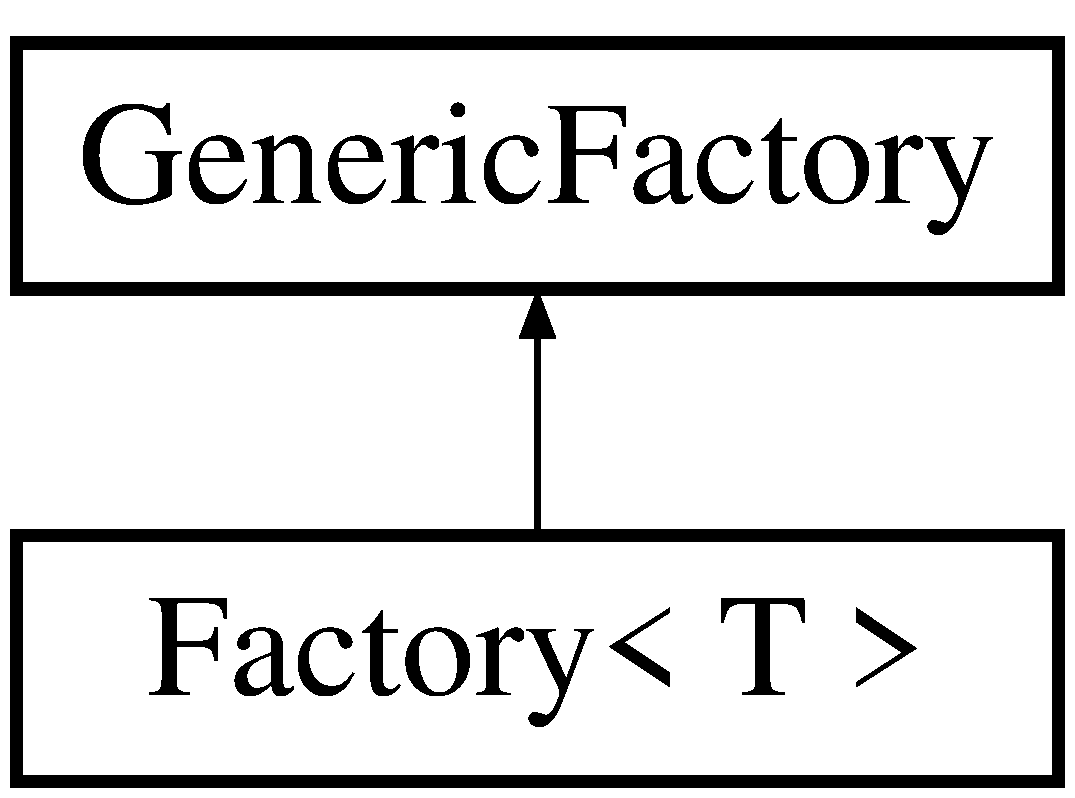
\includegraphics[height=2.000000cm]{class_factory}
\end{center}
\end{figure}
\subsection*{Public Member Functions}
\begin{DoxyCompactItemize}
\item 
\mbox{\Hypertarget{class_factory_a6c7dcfb9ba1de182fcd6b2e0990d02f3}\label{class_factory_a6c7dcfb9ba1de182fcd6b2e0990d02f3}} 
\hyperlink{class_color}{Color} $\ast$ {\bfseries get\+New\+Color} () const
\item 
\mbox{\Hypertarget{class_factory_a4bfca7f98466684ad447c753b678628a}\label{class_factory_a4bfca7f98466684ad447c753b678628a}} 
\hyperlink{class_color}{Color} $\ast$ {\bfseries get\+New\+Color} (const \hyperlink{class_color}{Color} $\ast$color) const
\end{DoxyCompactItemize}


The documentation for this class was generated from the following file\+:\begin{DoxyCompactItemize}
\item 
/home/gian/\+Projects/\+Kalk2-\/0/\+Kalk/\+Model/\+Factory/\hyperlink{factory_8h}{factory.\+h}\end{DoxyCompactItemize}

\hypertarget{class_factory_3_01_t_01_4}{}\section{Factory$<$ T $>$ Class Reference}
\label{class_factory_3_01_t_01_4}\index{Factory$<$ T $>$@{Factory$<$ T $>$}}


this class extends \hyperlink{class_generic_factory}{Generic\+Factory} and implements get\+New\+Color() and get\+New\+Color(const Color$\ast$ color) inizializes the map all\+Color\+Factories in \hyperlink{class_color_factory}{Color\+Factory} and makes available to \hyperlink{class_color_factory}{Color\+Factory} a constructor for the new color requested  




{\ttfamily \#include $<$factory.\+h$>$}



\subsection{Detailed Description}
this class extends \hyperlink{class_generic_factory}{Generic\+Factory} and implements get\+New\+Color() and get\+New\+Color(const Color$\ast$ color) inizializes the map all\+Color\+Factories in \hyperlink{class_color_factory}{Color\+Factory} and makes available to \hyperlink{class_color_factory}{Color\+Factory} a constructor for the new color requested 

this class is uses as base object to recall a Factory$<$t$>$ get\+New\+Color 

The documentation for this class was generated from the following file\+:\begin{DoxyCompactItemize}
\item 
/home/gian/\+Projects/\+Kalk2-\/0/\+Kalk/\+Model/\+Factory/\hyperlink{factory_8h}{factory.\+h}\end{DoxyCompactItemize}

\hypertarget{class_generic_factory}{}\section{Generic\+Factory Class Reference}
\label{class_generic_factory}\index{Generic\+Factory@{Generic\+Factory}}
Inheritance diagram for Generic\+Factory\+:\begin{figure}[H]
\begin{center}
\leavevmode
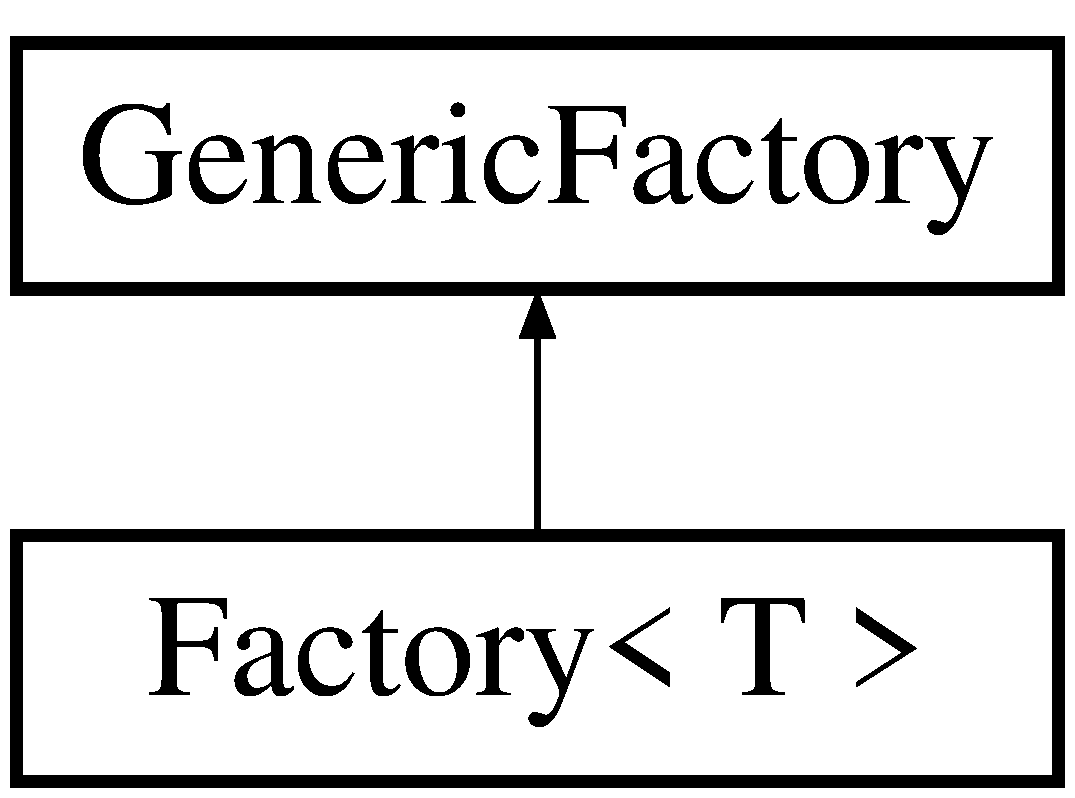
\includegraphics[height=2.000000cm]{class_generic_factory}
\end{center}
\end{figure}
\subsection*{Public Member Functions}
\begin{DoxyCompactItemize}
\item 
\mbox{\Hypertarget{class_generic_factory_a1e4a2993cb1684a24ed3edfb06efdaed}\label{class_generic_factory_a1e4a2993cb1684a24ed3edfb06efdaed}} 
virtual \hyperlink{class_color}{Color} $\ast$ {\bfseries get\+New\+Color} () const =0
\item 
\mbox{\Hypertarget{class_generic_factory_a478ac68c07e43943450d76babc963bab}\label{class_generic_factory_a478ac68c07e43943450d76babc963bab}} 
virtual \hyperlink{class_color}{Color} $\ast$ {\bfseries get\+New\+Color} (const \hyperlink{class_color}{Color} $\ast$color) const =0
\end{DoxyCompactItemize}


The documentation for this class was generated from the following file\+:\begin{DoxyCompactItemize}
\item 
/home/gian/\+Projects/\+Kalk2-\/0/\+Kalk/\+Model/\+Factory/\hyperlink{genericfactory_8h}{genericfactory.\+h}\end{DoxyCompactItemize}

\hypertarget{class_history_window}{}\section{History\+Window Class Reference}
\label{class_history_window}\index{History\+Window@{History\+Window}}
Inheritance diagram for History\+Window\+:\begin{figure}[H]
\begin{center}
\leavevmode
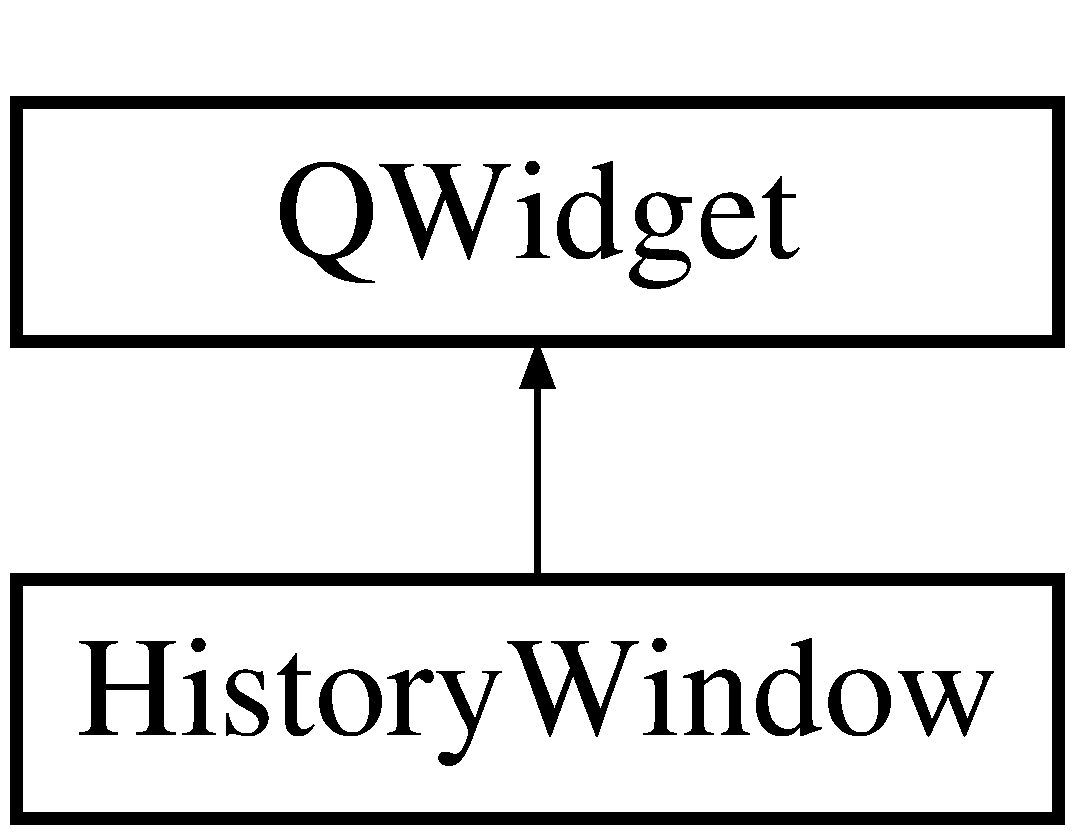
\includegraphics[height=2.000000cm]{class_history_window}
\end{center}
\end{figure}
\subsection*{Public Slots}
\begin{DoxyCompactItemize}
\item 
void \hyperlink{class_history_window_aa1baf09cc1f8dfc65b3647ca783cef43}{change\+Op} (int operation)
\begin{DoxyCompactList}\small\item\em \hyperlink{class_history_window_aa1baf09cc1f8dfc65b3647ca783cef43}{History\+Window\+::change\+Op} changes the window\textquotesingle{}s content. \end{DoxyCompactList}\item 
\mbox{\Hypertarget{class_history_window_a89fea4903efe8657ad735374255b317e}\label{class_history_window_a89fea4903efe8657ad735374255b317e}} 
void \hyperlink{class_history_window_a89fea4903efe8657ad735374255b317e}{add\+Menu\+History} ()
\begin{DoxyCompactList}\small\item\em \hyperlink{class_history_window_a89fea4903efe8657ad735374255b317e}{History\+Window\+::add\+Menu\+History} add entries. \end{DoxyCompactList}\end{DoxyCompactItemize}
\subsection*{Public Member Functions}
\begin{DoxyCompactItemize}
\item 
\hyperlink{class_history_window_ad545b50ee9a83c213221b3d937252d31}{History\+Window} (const Q\+Vector$<$ Q\+Vector$<$ Q\+String $>$$>$ \&history, Q\+Widget $\ast$parent=nullptr)
\begin{DoxyCompactList}\small\item\em \hyperlink{class_history_window_ad545b50ee9a83c213221b3d937252d31}{History\+Window\+::\+History\+Window}. \end{DoxyCompactList}\item 
\mbox{\Hypertarget{class_history_window_afc23bcc3cd1a50efa9d26bfafedc44b6}\label{class_history_window_afc23bcc3cd1a50efa9d26bfafedc44b6}} 
\hyperlink{class_history_window_afc23bcc3cd1a50efa9d26bfafedc44b6}{$\sim$\+History\+Window} ()
\begin{DoxyCompactList}\small\item\em \hyperlink{class_history_window_afc23bcc3cd1a50efa9d26bfafedc44b6}{History\+Window\+::$\sim$\+History\+Window}. \end{DoxyCompactList}\end{DoxyCompactItemize}


\subsection{Constructor \& Destructor Documentation}
\mbox{\Hypertarget{class_history_window_ad545b50ee9a83c213221b3d937252d31}\label{class_history_window_ad545b50ee9a83c213221b3d937252d31}} 
\index{History\+Window@{History\+Window}!History\+Window@{History\+Window}}
\index{History\+Window@{History\+Window}!History\+Window@{History\+Window}}
\subsubsection{\texorpdfstring{History\+Window()}{HistoryWindow()}}
{\footnotesize\ttfamily History\+Window\+::\+History\+Window (\begin{DoxyParamCaption}\item[{const Q\+Vector$<$ Q\+Vector$<$ Q\+String $>$$>$ \&}]{history,  }\item[{Q\+Widget $\ast$}]{parent = {\ttfamily nullptr} }\end{DoxyParamCaption})}



\hyperlink{class_history_window_ad545b50ee9a83c213221b3d937252d31}{History\+Window\+::\+History\+Window}. 


\begin{DoxyParams}{Parameters}
{\em history} & \\
\hline
{\em parent} & \\
\hline
\end{DoxyParams}


\subsection{Member Function Documentation}
\mbox{\Hypertarget{class_history_window_aa1baf09cc1f8dfc65b3647ca783cef43}\label{class_history_window_aa1baf09cc1f8dfc65b3647ca783cef43}} 
\index{History\+Window@{History\+Window}!change\+Op@{change\+Op}}
\index{change\+Op@{change\+Op}!History\+Window@{History\+Window}}
\subsubsection{\texorpdfstring{change\+Op}{changeOp}}
{\footnotesize\ttfamily void History\+Window\+::change\+Op (\begin{DoxyParamCaption}\item[{int}]{operation }\end{DoxyParamCaption})\hspace{0.3cm}{\ttfamily [slot]}}



\hyperlink{class_history_window_aa1baf09cc1f8dfc65b3647ca783cef43}{History\+Window\+::change\+Op} changes the window\textquotesingle{}s content. 


\begin{DoxyParams}{Parameters}
{\em operation} & \\
\hline
\end{DoxyParams}


The documentation for this class was generated from the following files\+:\begin{DoxyCompactItemize}
\item 
/home/gian/\+Projects/\+Kalk2-\/0/\+Kalk/\+View/\+Gui/\hyperlink{historywindow_8h}{historywindow.\+h}\item 
/home/gian/\+Projects/\+Kalk2-\/0/\+Kalk/\+View/\+Gui/historywindow.\+cpp\end{DoxyCompactItemize}

\hypertarget{class_h_s_l}{}\section{H\+SL Class Reference}
\label{class_h_s_l}\index{H\+SL@{H\+SL}}


this class uses as base the class \hyperlink{class_c_i_exyz}{C\+I\+Exyz} \hyperlink{class_h_s_l}{H\+SL} stores a color in \hyperlink{class_h_s_l}{H\+SL} representation  




{\ttfamily \#include $<$hsl.\+h$>$}

Inheritance diagram for H\+SL\+:\begin{figure}[H]
\begin{center}
\leavevmode
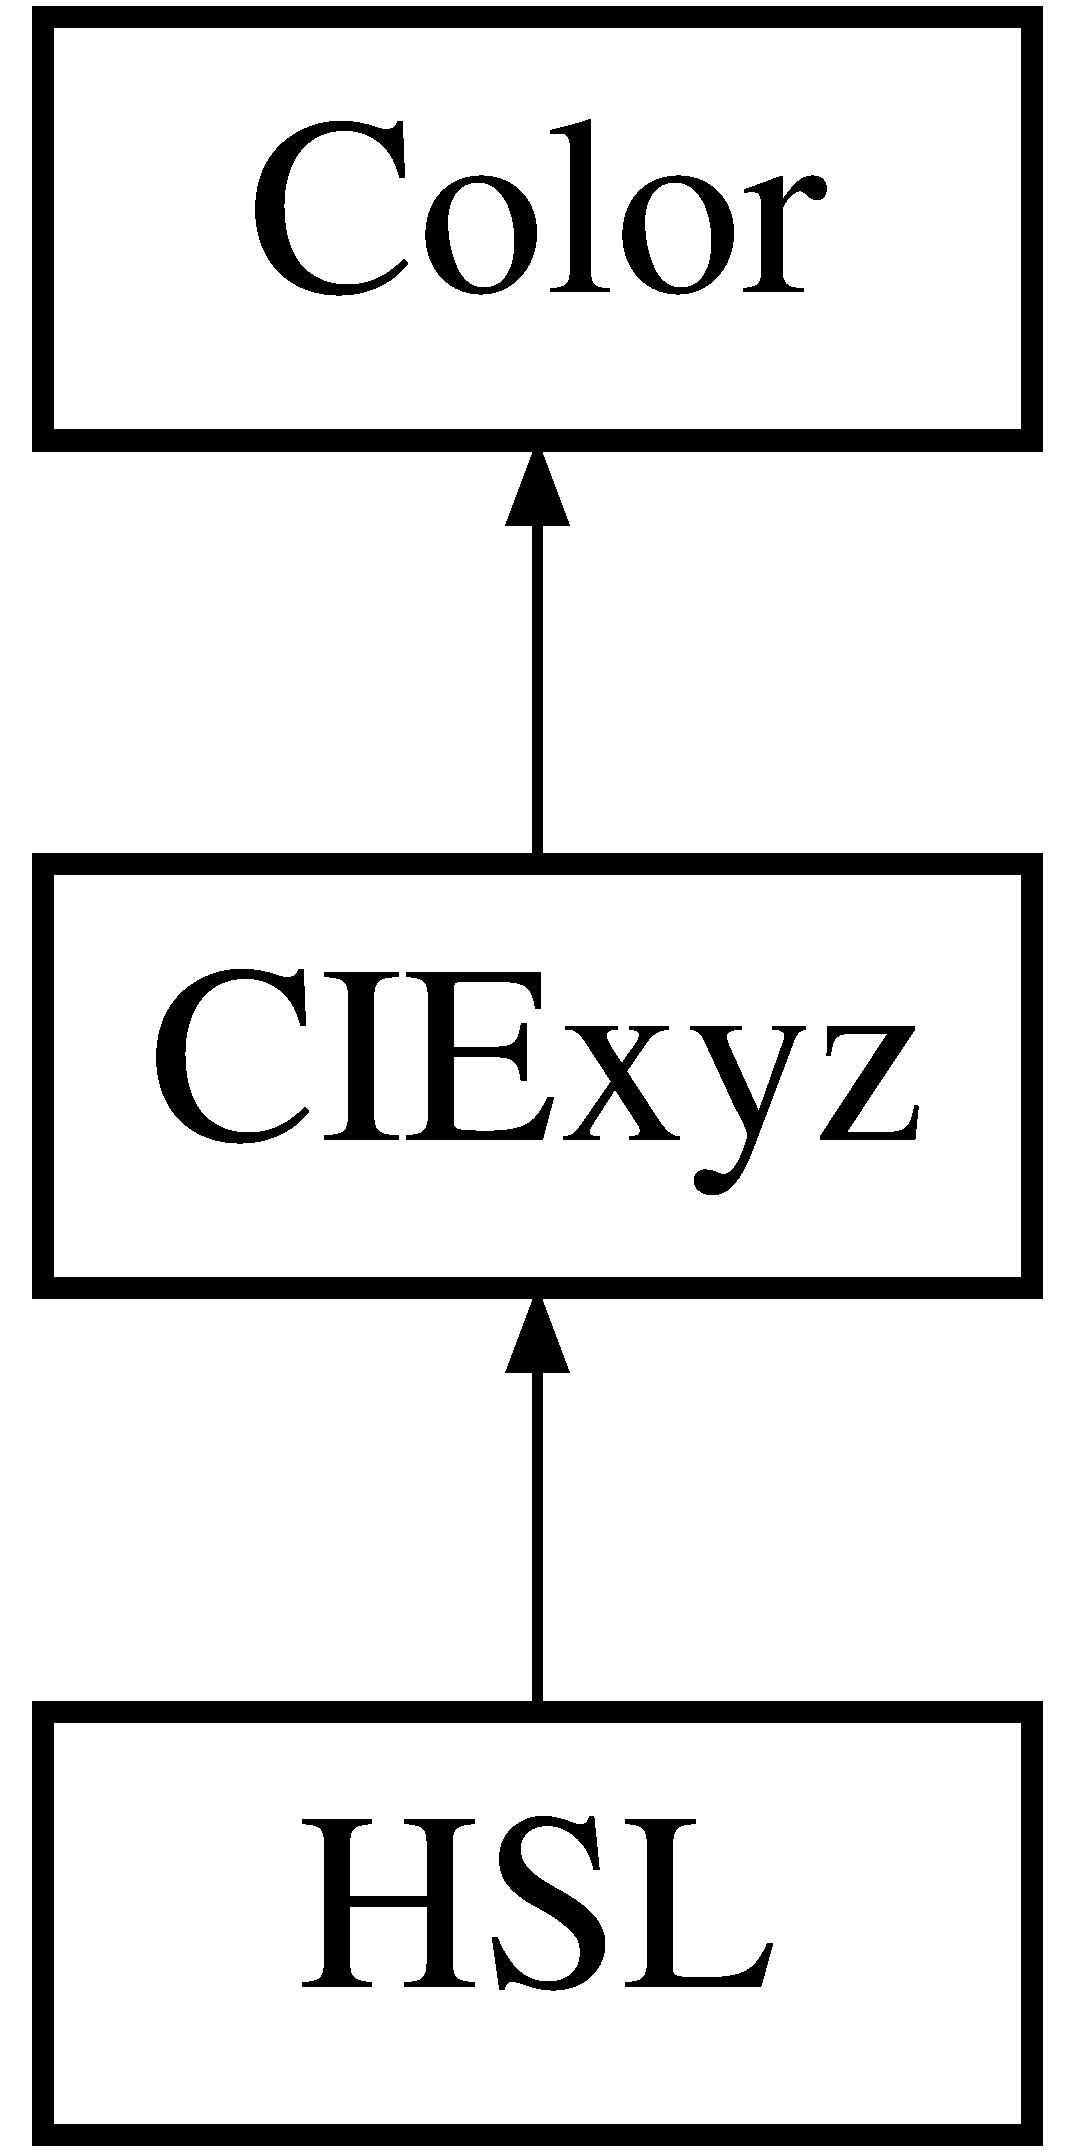
\includegraphics[height=3.000000cm]{class_h_s_l}
\end{center}
\end{figure}
\subsection*{Public Member Functions}
\begin{DoxyCompactItemize}
\item 
\hyperlink{class_h_s_l_af90e79ad88ecb7944c313330d4bde182}{H\+SL} (double h=0, double s=0, double l=0)
\begin{DoxyCompactList}\small\item\em \hyperlink{class_h_s_l_af90e79ad88ecb7944c313330d4bde182}{H\+S\+L\+::\+H\+SL} Constructor for \hyperlink{class_h_s_l}{H\+SL} color representation from double precision numbers. \end{DoxyCompactList}\item 
\hyperlink{class_h_s_l_ae737a28ec6a67bba89090c9a63c5cc21}{H\+SL} (const \hyperlink{class_color}{Color} $\ast$from)
\begin{DoxyCompactList}\small\item\em \hyperlink{class_h_s_l_af90e79ad88ecb7944c313330d4bde182}{H\+S\+L\+::\+H\+SL} Constructor for \hyperlink{class_h_s_l}{H\+SL} color representation from \hyperlink{class_color}{Color} pointer. \end{DoxyCompactList}\item 
\hyperlink{class_h_s_l_a165c0123fc7294e7ccdc53fc11c57154}{H\+SL} (const \hyperlink{class_h_s_l}{H\+SL} \&from)
\begin{DoxyCompactList}\small\item\em \hyperlink{class_h_s_l_af90e79ad88ecb7944c313330d4bde182}{H\+S\+L\+::\+H\+SL} copy constructor. \end{DoxyCompactList}\item 
Q\+String \hyperlink{class_h_s_l_a774dc0a5dad87bc9ff44956af4873602}{get\+Representation} () const
\begin{DoxyCompactList}\small\item\em H\+S\+L\+::getrepresentation. \end{DoxyCompactList}\item 
\hyperlink{class_color}{Color} $\ast$ \hyperlink{class_h_s_l_af681f885d11220b0588e8f969aa95e32}{negate} () const
\begin{DoxyCompactList}\small\item\em \hyperlink{class_h_s_l_af681f885d11220b0588e8f969aa95e32}{H\+S\+L\+::negate}. \end{DoxyCompactList}\item 
\hyperlink{class_color}{Color} $\ast$ \hyperlink{class_h_s_l_a08bcec2ca6961b7c6431d92a625c30a7}{mix} (const \hyperlink{class_color}{Color} $\ast$a) const
\begin{DoxyCompactList}\small\item\em \hyperlink{class_h_s_l_a08bcec2ca6961b7c6431d92a625c30a7}{H\+S\+L\+::mix}. \end{DoxyCompactList}\item 
\hyperlink{class_color}{Color} $\ast$ \hyperlink{class_h_s_l_ad755c96eff0cc73dea69c007d745dd4e}{get\+C\+IE} (double h, double s, double l) const
\begin{DoxyCompactList}\small\item\em \hyperlink{class_h_s_l_ad755c96eff0cc73dea69c007d745dd4e}{H\+S\+L\+::get\+C\+IE}. \end{DoxyCompactList}\item 
Q\+Vector$<$ double $>$ \hyperlink{class_h_s_l_a2de2eb4fa5c9ffcea894f7c6591cb335}{get\+Components} () const
\begin{DoxyCompactList}\small\item\em H\+S\+L\+::get\+Component. \end{DoxyCompactList}\item 
void \hyperlink{class_h_s_l_a101be14729707abca388680610e2fe86}{set\+Components} (Q\+Vector$<$ double $>$ componets)
\begin{DoxyCompactList}\small\item\em \hyperlink{class_h_s_l_a101be14729707abca388680610e2fe86}{H\+S\+L\+::set\+Components} set the components inside the object. \end{DoxyCompactList}\item 
int \hyperlink{class_h_s_l_a6e582f5779c1b5f84abe8bb182a868d0}{get\+Number\+Of\+Componets} () const
\begin{DoxyCompactList}\small\item\em \hyperlink{class_h_s_l_a6e582f5779c1b5f84abe8bb182a868d0}{H\+S\+L\+::get\+Number\+Of\+Componets}. \end{DoxyCompactList}\item 
Q\+Vector$<$ Q\+String $>$ \hyperlink{class_h_s_l_a7ac26d7b7b5755769165455e1b6d3312}{get\+Limits} () const
\begin{DoxyCompactList}\small\item\em \hyperlink{class_h_s_l_a7ac26d7b7b5755769165455e1b6d3312}{H\+S\+L\+::get\+Limits}. \end{DoxyCompactList}\end{DoxyCompactItemize}
\subsection*{Additional Inherited Members}


\subsection{Detailed Description}
this class uses as base the class \hyperlink{class_c_i_exyz}{C\+I\+Exyz} \hyperlink{class_h_s_l}{H\+SL} stores a color in \hyperlink{class_h_s_l}{H\+SL} representation 

\subsection{Constructor \& Destructor Documentation}
\mbox{\Hypertarget{class_h_s_l_af90e79ad88ecb7944c313330d4bde182}\label{class_h_s_l_af90e79ad88ecb7944c313330d4bde182}} 
\index{H\+SL@{H\+SL}!H\+SL@{H\+SL}}
\index{H\+SL@{H\+SL}!H\+SL@{H\+SL}}
\subsubsection{\texorpdfstring{H\+S\+L()}{HSL()}\hspace{0.1cm}{\footnotesize\ttfamily [1/3]}}
{\footnotesize\ttfamily H\+S\+L\+::\+H\+SL (\begin{DoxyParamCaption}\item[{double}]{h = {\ttfamily 0},  }\item[{double}]{s = {\ttfamily 0},  }\item[{double}]{l = {\ttfamily 0} }\end{DoxyParamCaption})}



\hyperlink{class_h_s_l_af90e79ad88ecb7944c313330d4bde182}{H\+S\+L\+::\+H\+SL} Constructor for \hyperlink{class_h_s_l}{H\+SL} color representation from double precision numbers. 


\begin{DoxyParams}{Parameters}
{\em h} & \\
\hline
{\em s} & \\
\hline
{\em l} & \\
\hline
\end{DoxyParams}
\mbox{\Hypertarget{class_h_s_l_ae737a28ec6a67bba89090c9a63c5cc21}\label{class_h_s_l_ae737a28ec6a67bba89090c9a63c5cc21}} 
\index{H\+SL@{H\+SL}!H\+SL@{H\+SL}}
\index{H\+SL@{H\+SL}!H\+SL@{H\+SL}}
\subsubsection{\texorpdfstring{H\+S\+L()}{HSL()}\hspace{0.1cm}{\footnotesize\ttfamily [2/3]}}
{\footnotesize\ttfamily H\+S\+L\+::\+H\+SL (\begin{DoxyParamCaption}\item[{const \hyperlink{class_color}{Color} $\ast$}]{from }\end{DoxyParamCaption})}



\hyperlink{class_h_s_l_af90e79ad88ecb7944c313330d4bde182}{H\+S\+L\+::\+H\+SL} Constructor for \hyperlink{class_h_s_l}{H\+SL} color representation from \hyperlink{class_color}{Color} pointer. 


\begin{DoxyParams}{Parameters}
{\em from} & \\
\hline
\end{DoxyParams}
\mbox{\Hypertarget{class_h_s_l_a165c0123fc7294e7ccdc53fc11c57154}\label{class_h_s_l_a165c0123fc7294e7ccdc53fc11c57154}} 
\index{H\+SL@{H\+SL}!H\+SL@{H\+SL}}
\index{H\+SL@{H\+SL}!H\+SL@{H\+SL}}
\subsubsection{\texorpdfstring{H\+S\+L()}{HSL()}\hspace{0.1cm}{\footnotesize\ttfamily [3/3]}}
{\footnotesize\ttfamily H\+S\+L\+::\+H\+SL (\begin{DoxyParamCaption}\item[{const \hyperlink{class_h_s_l}{H\+SL} \&}]{from }\end{DoxyParamCaption})}



\hyperlink{class_h_s_l_af90e79ad88ecb7944c313330d4bde182}{H\+S\+L\+::\+H\+SL} copy constructor. 


\begin{DoxyParams}{Parameters}
{\em from} & \\
\hline
\end{DoxyParams}


\subsection{Member Function Documentation}
\mbox{\Hypertarget{class_h_s_l_ad755c96eff0cc73dea69c007d745dd4e}\label{class_h_s_l_ad755c96eff0cc73dea69c007d745dd4e}} 
\index{H\+SL@{H\+SL}!get\+C\+IE@{get\+C\+IE}}
\index{get\+C\+IE@{get\+C\+IE}!H\+SL@{H\+SL}}
\subsubsection{\texorpdfstring{get\+C\+I\+E()}{getCIE()}}
{\footnotesize\ttfamily \hyperlink{class_color}{Color} $\ast$ H\+S\+L\+::get\+C\+IE (\begin{DoxyParamCaption}\item[{double}]{h,  }\item[{double}]{s,  }\item[{double}]{l }\end{DoxyParamCaption}) const}



\hyperlink{class_h_s_l_ad755c96eff0cc73dea69c007d745dd4e}{H\+S\+L\+::get\+C\+IE}. 


\begin{DoxyParams}{Parameters}
{\em h} & \\
\hline
{\em s} & \\
\hline
{\em l} & \\
\hline
\end{DoxyParams}

\begin{DoxyExceptions}{Exceptions}
{\em \hyperlink{class_illegal_color_exception}{Illegal\+Color\+Exception}} & \\
\hline
\end{DoxyExceptions}
\begin{DoxyReturn}{Returns}
\hyperlink{class_color}{Color} pointer with a clone of $\ast$this in the \hyperlink{class_c_i_exyz}{C\+I\+Exyz} format 
\end{DoxyReturn}
\mbox{\Hypertarget{class_h_s_l_a2de2eb4fa5c9ffcea894f7c6591cb335}\label{class_h_s_l_a2de2eb4fa5c9ffcea894f7c6591cb335}} 
\index{H\+SL@{H\+SL}!get\+Components@{get\+Components}}
\index{get\+Components@{get\+Components}!H\+SL@{H\+SL}}
\subsubsection{\texorpdfstring{get\+Components()}{getComponents()}}
{\footnotesize\ttfamily Q\+Vector$<$ double $>$ H\+S\+L\+::get\+Components (\begin{DoxyParamCaption}{ }\end{DoxyParamCaption}) const\hspace{0.3cm}{\ttfamily [virtual]}}



H\+S\+L\+::get\+Component. 

\begin{DoxyReturn}{Returns}
Q\+Vector$<$double$>$ with the hue, saturation, lightness component of the color in \hyperlink{class_h_s_l}{H\+SL} 
\end{DoxyReturn}


Reimplemented from \hyperlink{class_c_i_exyz_af8992e3ac1741c35fcb18aa2cdb554a0}{C\+I\+Exyz}.

\mbox{\Hypertarget{class_h_s_l_a7ac26d7b7b5755769165455e1b6d3312}\label{class_h_s_l_a7ac26d7b7b5755769165455e1b6d3312}} 
\index{H\+SL@{H\+SL}!get\+Limits@{get\+Limits}}
\index{get\+Limits@{get\+Limits}!H\+SL@{H\+SL}}
\subsubsection{\texorpdfstring{get\+Limits()}{getLimits()}}
{\footnotesize\ttfamily Q\+Vector$<$ Q\+String $>$ H\+S\+L\+::get\+Limits (\begin{DoxyParamCaption}{ }\end{DoxyParamCaption}) const\hspace{0.3cm}{\ttfamily [virtual]}}



\hyperlink{class_h_s_l_a7ac26d7b7b5755769165455e1b6d3312}{H\+S\+L\+::get\+Limits}. 

\begin{DoxyReturn}{Returns}
limits of \hyperlink{class_h_s_l}{H\+SL} as Q\+Vector$<$\+Q\+String$>$ 
\end{DoxyReturn}


Reimplemented from \hyperlink{class_c_i_exyz_a4c3aa6777f7720ae26b53174322a83f8}{C\+I\+Exyz}.

\mbox{\Hypertarget{class_h_s_l_a6e582f5779c1b5f84abe8bb182a868d0}\label{class_h_s_l_a6e582f5779c1b5f84abe8bb182a868d0}} 
\index{H\+SL@{H\+SL}!get\+Number\+Of\+Componets@{get\+Number\+Of\+Componets}}
\index{get\+Number\+Of\+Componets@{get\+Number\+Of\+Componets}!H\+SL@{H\+SL}}
\subsubsection{\texorpdfstring{get\+Number\+Of\+Componets()}{getNumberOfComponets()}}
{\footnotesize\ttfamily int H\+S\+L\+::get\+Number\+Of\+Componets (\begin{DoxyParamCaption}{ }\end{DoxyParamCaption}) const\hspace{0.3cm}{\ttfamily [virtual]}}



\hyperlink{class_h_s_l_a6e582f5779c1b5f84abe8bb182a868d0}{H\+S\+L\+::get\+Number\+Of\+Componets}. 

\begin{DoxyReturn}{Returns}
int componets number 
\end{DoxyReturn}


Reimplemented from \hyperlink{class_c_i_exyz_af168733bb1bca36a7ae5d75c67de046e}{C\+I\+Exyz}.

\mbox{\Hypertarget{class_h_s_l_a774dc0a5dad87bc9ff44956af4873602}\label{class_h_s_l_a774dc0a5dad87bc9ff44956af4873602}} 
\index{H\+SL@{H\+SL}!get\+Representation@{get\+Representation}}
\index{get\+Representation@{get\+Representation}!H\+SL@{H\+SL}}
\subsubsection{\texorpdfstring{get\+Representation()}{getRepresentation()}}
{\footnotesize\ttfamily Q\+String H\+S\+L\+::get\+Representation (\begin{DoxyParamCaption}{ }\end{DoxyParamCaption}) const\hspace{0.3cm}{\ttfamily [virtual]}}



H\+S\+L\+::getrepresentation. 

\begin{DoxyReturn}{Returns}
Q\+String that contains name of the object 
\end{DoxyReturn}


Reimplemented from \hyperlink{class_c_i_exyz_a19120c15d1304696909d76fae6065ebd}{C\+I\+Exyz}.

\mbox{\Hypertarget{class_h_s_l_a08bcec2ca6961b7c6431d92a625c30a7}\label{class_h_s_l_a08bcec2ca6961b7c6431d92a625c30a7}} 
\index{H\+SL@{H\+SL}!mix@{mix}}
\index{mix@{mix}!H\+SL@{H\+SL}}
\subsubsection{\texorpdfstring{mix()}{mix()}}
{\footnotesize\ttfamily \hyperlink{class_color}{Color} $\ast$ H\+S\+L\+::mix (\begin{DoxyParamCaption}\item[{const \hyperlink{class_color}{Color} $\ast$}]{a }\end{DoxyParamCaption}) const\hspace{0.3cm}{\ttfamily [virtual]}}



\hyperlink{class_h_s_l_a08bcec2ca6961b7c6431d92a625c30a7}{H\+S\+L\+::mix}. 


\begin{DoxyParams}{Parameters}
{\em a} & \\
\hline
\end{DoxyParams}
\begin{DoxyReturn}{Returns}
\hyperlink{class_color}{Color} pointer with a new color mixed as \hyperlink{class_h_s_l}{H\+SL} 
\end{DoxyReturn}


Reimplemented from \hyperlink{class_c_i_exyz_af8eeb48ade44beea43d023b36d263fc8}{C\+I\+Exyz}.

\mbox{\Hypertarget{class_h_s_l_af681f885d11220b0588e8f969aa95e32}\label{class_h_s_l_af681f885d11220b0588e8f969aa95e32}} 
\index{H\+SL@{H\+SL}!negate@{negate}}
\index{negate@{negate}!H\+SL@{H\+SL}}
\subsubsection{\texorpdfstring{negate()}{negate()}}
{\footnotesize\ttfamily \hyperlink{class_color}{Color} $\ast$ H\+S\+L\+::negate (\begin{DoxyParamCaption}{ }\end{DoxyParamCaption}) const\hspace{0.3cm}{\ttfamily [virtual]}}



\hyperlink{class_h_s_l_af681f885d11220b0588e8f969aa95e32}{H\+S\+L\+::negate}. 

\begin{DoxyReturn}{Returns}
\hyperlink{class_color}{Color} pointer with a new color with the negated values 
\end{DoxyReturn}


Reimplemented from \hyperlink{class_c_i_exyz_a4a454df6cbb71f3fcfd2d1ea9d500d94}{C\+I\+Exyz}.

\mbox{\Hypertarget{class_h_s_l_a101be14729707abca388680610e2fe86}\label{class_h_s_l_a101be14729707abca388680610e2fe86}} 
\index{H\+SL@{H\+SL}!set\+Components@{set\+Components}}
\index{set\+Components@{set\+Components}!H\+SL@{H\+SL}}
\subsubsection{\texorpdfstring{set\+Components()}{setComponents()}}
{\footnotesize\ttfamily void H\+S\+L\+::set\+Components (\begin{DoxyParamCaption}\item[{Q\+Vector$<$ double $>$}]{componets }\end{DoxyParamCaption})\hspace{0.3cm}{\ttfamily [virtual]}}



\hyperlink{class_h_s_l_a101be14729707abca388680610e2fe86}{H\+S\+L\+::set\+Components} set the components inside the object. 


\begin{DoxyExceptions}{Exceptions}
{\em \hyperlink{class_illegal_color_exception}{Illegal\+Color\+Exception}} & \\
\hline
\end{DoxyExceptions}

\begin{DoxyParams}{Parameters}
{\em componets} & \\
\hline
\end{DoxyParams}


Reimplemented from \hyperlink{class_c_i_exyz_a11468574f91d2cb1356f0cde56429b84}{C\+I\+Exyz}.



The documentation for this class was generated from the following files\+:\begin{DoxyCompactItemize}
\item 
/home/gian/\+Projects/\+Kalk2-\/0/\+Kalk/\+Model/\+Color/\+H\+S\+L/\hyperlink{hsl_8h}{hsl.\+h}\item 
/home/gian/\+Projects/\+Kalk2-\/0/\+Kalk/\+Model/\+Color/\+H\+S\+L/hsl.\+cpp\end{DoxyCompactItemize}

\hypertarget{class_illegal_color_exception}{}\section{Illegal\+Color\+Exception Class Reference}
\label{class_illegal_color_exception}\index{Illegal\+Color\+Exception@{Illegal\+Color\+Exception}}
Inheritance diagram for Illegal\+Color\+Exception\+:\begin{figure}[H]
\begin{center}
\leavevmode
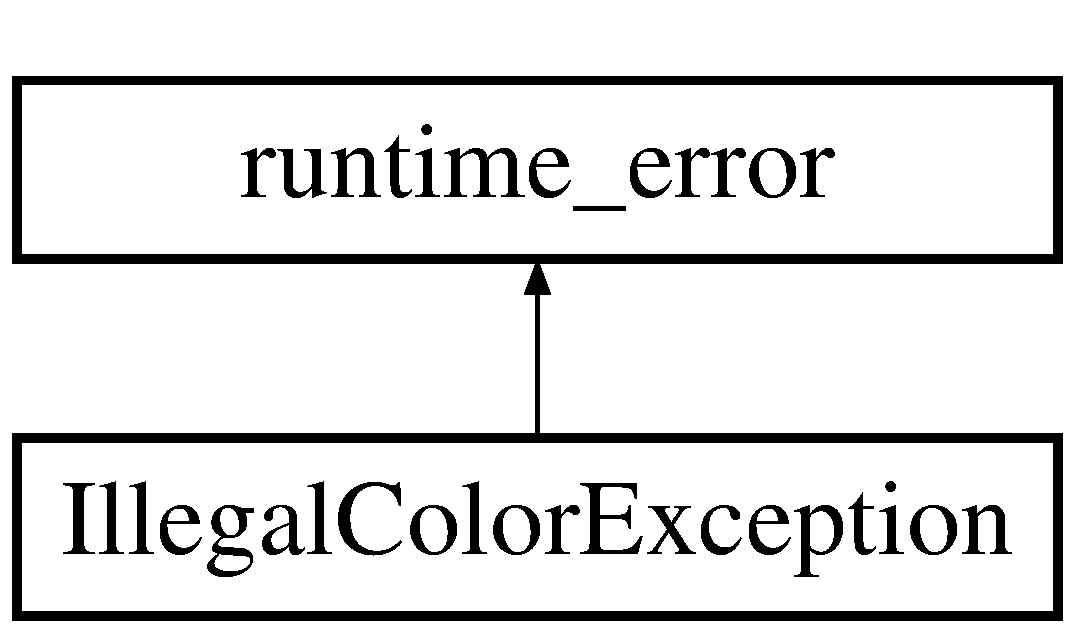
\includegraphics[height=2.000000cm]{class_illegal_color_exception}
\end{center}
\end{figure}
\subsection*{Public Member Functions}
\begin{DoxyCompactItemize}
\item 
\mbox{\Hypertarget{class_illegal_color_exception_a2d06f0597577dae21d50835a9e95e531}\label{class_illegal_color_exception_a2d06f0597577dae21d50835a9e95e531}} 
{\bfseries Illegal\+Color\+Exception} (std\+::string e)
\end{DoxyCompactItemize}


The documentation for this class was generated from the following file\+:\begin{DoxyCompactItemize}
\item 
/home/gian/\+Projects/\+Kalk2-\/0/\+Kalk/\+Model/\hyperlink{illegalcolorexception_8h}{illegalcolorexception.\+h}\end{DoxyCompactItemize}

\hypertarget{class_main_window}{}\section{Main\+Window Class Reference}
\label{class_main_window}\index{Main\+Window@{Main\+Window}}
Inheritance diagram for Main\+Window\+:\begin{figure}[H]
\begin{center}
\leavevmode
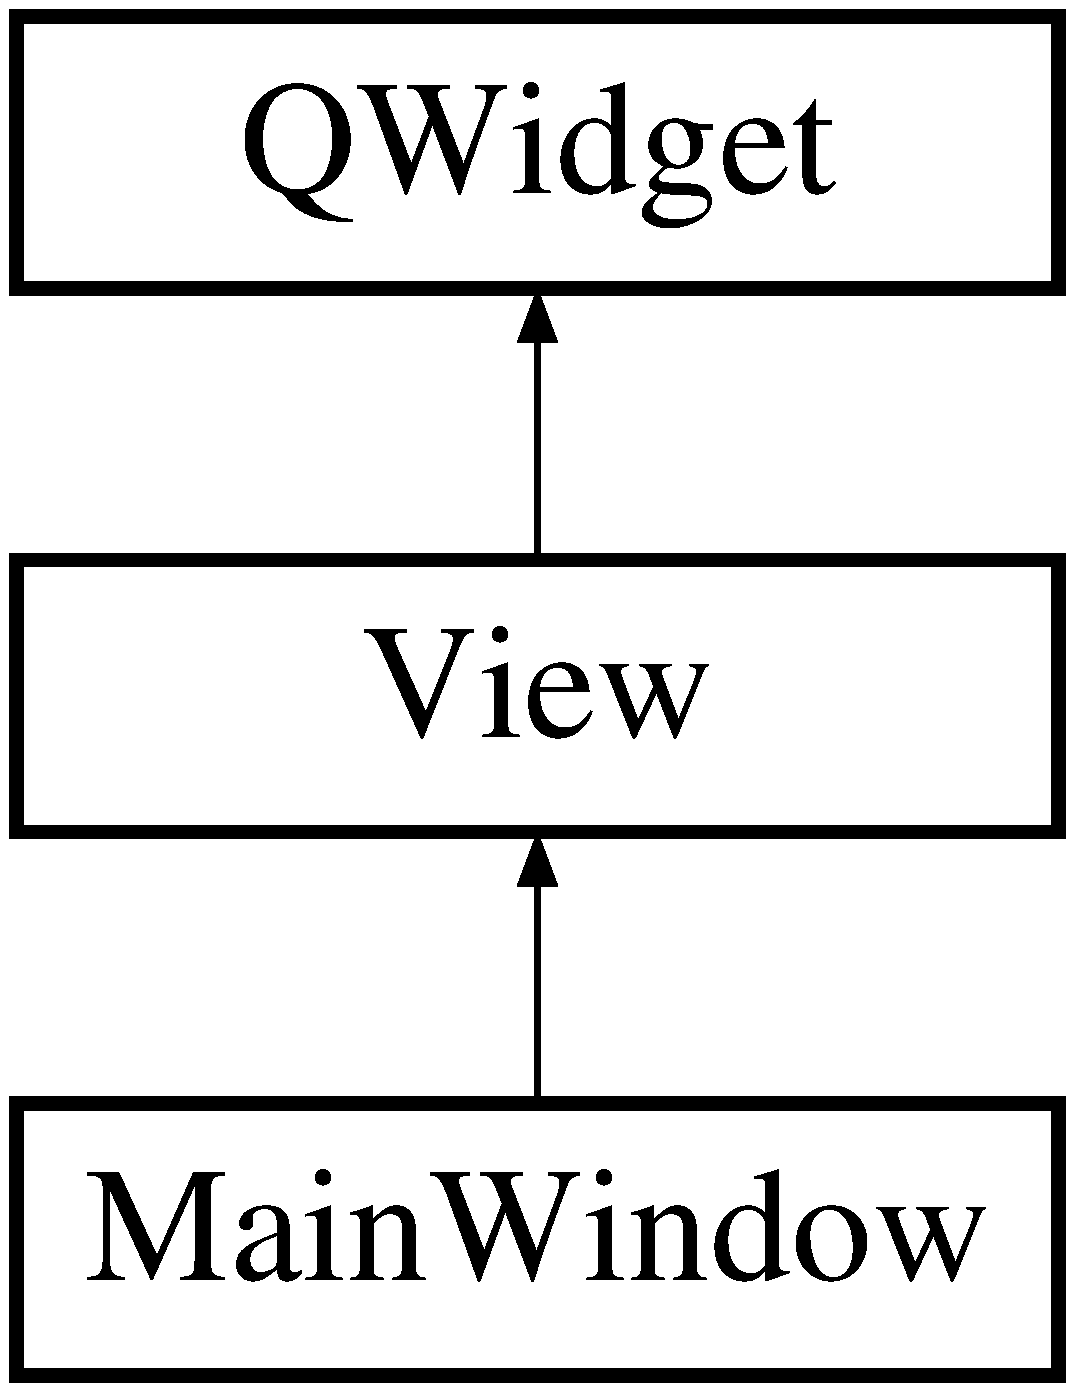
\includegraphics[height=3.000000cm]{class_main_window}
\end{center}
\end{figure}
\subsection*{Public Slots}
\begin{DoxyCompactItemize}
\item 
void \hyperlink{class_main_window_ae065551040ada6411fc1fb4f3887dd3b}{set\+Left\+Types} (const Q\+Vector$<$ Q\+String $>$ types)
\begin{DoxyCompactList}\small\item\em \hyperlink{class_main_window_ae065551040ada6411fc1fb4f3887dd3b}{Main\+Window\+::set\+Left\+Types} add various types to the left drop menu. \end{DoxyCompactList}\item 
void \hyperlink{class_main_window_aca464c6893a9551372c043cb3bf7bf56}{set\+Right\+Types} (const Q\+Vector$<$ Q\+String $>$ types)
\begin{DoxyCompactList}\small\item\em \hyperlink{class_main_window_aca464c6893a9551372c043cb3bf7bf56}{Main\+Window\+::set\+Right\+Types} add various types to the right drop menu. \end{DoxyCompactList}\item 
void \hyperlink{class_main_window_a5e2ad194f3764cb9a321b01193c53be9}{set\+Result\+Types} (const Q\+Vector$<$ Q\+String $>$ types)
\begin{DoxyCompactList}\small\item\em \hyperlink{class_main_window_a5e2ad194f3764cb9a321b01193c53be9}{Main\+Window\+::set\+Result\+Types} add various types to the result drop menu. \end{DoxyCompactList}\item 
void \hyperlink{class_main_window_a48d094bc4e7965be372f62d2f6e6d910}{set\+Left\+Fields} (const int \&fields, const Q\+Vector$<$ Q\+String $>$ \&limits)
\begin{DoxyCompactList}\small\item\em \hyperlink{class_main_window_a48d094bc4e7965be372f62d2f6e6d910}{Main\+Window\+::set\+Left\+Fields} add \#fields entry lines for the selected left type. \end{DoxyCompactList}\item 
void \hyperlink{class_main_window_a8cbaa03b855c6ab3bb7a910662346549}{set\+Right\+Fields} (const int \&fields, const Q\+Vector$<$ Q\+String $>$ \&limits)
\begin{DoxyCompactList}\small\item\em \hyperlink{class_main_window_a8cbaa03b855c6ab3bb7a910662346549}{Main\+Window\+::set\+Right\+Fields} add \#fields entry lines for the selected right type. \end{DoxyCompactList}\item 
void \hyperlink{class_main_window_ae00d4afec436d34430e43dcc6742b875}{set\+Result\+Fields} (const int \&fields)
\begin{DoxyCompactList}\small\item\em \hyperlink{class_main_window_ae00d4afec436d34430e43dcc6742b875}{Main\+Window\+::set\+Result\+Fields} add \#fields lines for the result. \end{DoxyCompactList}\item 
void \hyperlink{class_main_window_a282ffcc1cb28b83d4f8fe510f6b2e42e}{set\+Available\+Operations} (const Q\+Vector$<$ Q\+String $>$ operations)
\begin{DoxyCompactList}\small\item\em \hyperlink{class_main_window_a282ffcc1cb28b83d4f8fe510f6b2e42e}{Main\+Window\+::set\+Available\+Operations} create and connect the given operation to the buttons. \end{DoxyCompactList}\item 
void \hyperlink{class_main_window_a86f711960ec362153b5d2ef6667c6c0c}{set\+Permitted\+Operations} (const Q\+Vector$<$ Q\+String $>$ operations)
\begin{DoxyCompactList}\small\item\em \hyperlink{class_main_window_a86f711960ec362153b5d2ef6667c6c0c}{Main\+Window\+::set\+Permitted\+Operations} toggle the operation buttons that are not aviable for that type. \end{DoxyCompactList}\item 
void \hyperlink{class_main_window_a04fa84f042da5f258d1dc09803667bbf}{set\+Result} (const Q\+Vector$<$ Q\+String $>$ result)
\begin{DoxyCompactList}\small\item\em \hyperlink{class_main_window_a04fa84f042da5f258d1dc09803667bbf}{Main\+Window\+::set\+Result} shows the recived result in the appropriate line. \end{DoxyCompactList}\item 
\mbox{\Hypertarget{class_main_window_aa16f2c84e4ddda0e0544e1e189b3bc62}\label{class_main_window_aa16f2c84e4ddda0e0544e1e189b3bc62}} 
void \hyperlink{class_main_window_aa16f2c84e4ddda0e0544e1e189b3bc62}{set\+Num\+Pad} ()
\begin{DoxyCompactList}\small\item\em \hyperlink{class_main_window_aa16f2c84e4ddda0e0544e1e189b3bc62}{Main\+Window\+::set\+Num\+Pad} set the numbers buttons and the utility buttons, then connect them to the appropriate input. \end{DoxyCompactList}\item 
void \hyperlink{class_main_window_ace7360a427c4d1b9a5252bd7a468510d}{set\+History} (const Q\+Vector$<$ Q\+Vector$<$ Q\+String $>$$>$ \&history)
\begin{DoxyCompactList}\small\item\em \hyperlink{class_main_window_ace7360a427c4d1b9a5252bd7a468510d}{Main\+Window\+::set\+History} create a new window with history. \end{DoxyCompactList}\item 
void \hyperlink{class_main_window_a8f2494aee2da70c23aff1c016c6b3225}{error} (const Q\+String \&error\+\_\+message)
\begin{DoxyCompactList}\small\item\em \hyperlink{class_main_window_a8f2494aee2da70c23aff1c016c6b3225}{Main\+Window\+::error} create a new window with error message. \end{DoxyCompactList}\item 
void \hyperlink{class_main_window_ae01409cebd6dcebf97ca2f4696fcf542}{reset\+Type} (Q\+String drop, Q\+String type)
\begin{DoxyCompactList}\small\item\em \hyperlink{class_main_window_ae01409cebd6dcebf97ca2f4696fcf542}{Main\+Window\+::reset\+Type}. \end{DoxyCompactList}\item 
\mbox{\Hypertarget{class_main_window_ae3d7a4598609a86e8bd317c0d85c4495}\label{class_main_window_ae3d7a4598609a86e8bd317c0d85c4495}} 
void \hyperlink{class_main_window_ae3d7a4598609a86e8bd317c0d85c4495}{show} ()
\begin{DoxyCompactList}\small\item\em \hyperlink{class_main_window_ae3d7a4598609a86e8bd317c0d85c4495}{Main\+Window\+::show} shows the windows. \end{DoxyCompactList}\end{DoxyCompactItemize}
\subsection*{Public Member Functions}
\begin{DoxyCompactItemize}
\item 
\hyperlink{class_main_window_a996c5a2b6f77944776856f08ec30858d}{Main\+Window} (Q\+Widget $\ast$parent=nullptr)
\begin{DoxyCompactList}\small\item\em \hyperlink{class_main_window_a996c5a2b6f77944776856f08ec30858d}{Main\+Window\+::\+Main\+Window} constructor. \end{DoxyCompactList}\item 
\mbox{\Hypertarget{class_main_window_ae98d00a93bc118200eeef9f9bba1dba7}\label{class_main_window_ae98d00a93bc118200eeef9f9bba1dba7}} 
\hyperlink{class_main_window_ae98d00a93bc118200eeef9f9bba1dba7}{$\sim$\+Main\+Window} ()
\begin{DoxyCompactList}\small\item\em \hyperlink{class_main_window_a996c5a2b6f77944776856f08ec30858d}{Main\+Window\+::\+Main\+Window} virtual destructor. \end{DoxyCompactList}\end{DoxyCompactItemize}
\subsection*{Additional Inherited Members}


\subsection{Constructor \& Destructor Documentation}
\mbox{\Hypertarget{class_main_window_a996c5a2b6f77944776856f08ec30858d}\label{class_main_window_a996c5a2b6f77944776856f08ec30858d}} 
\index{Main\+Window@{Main\+Window}!Main\+Window@{Main\+Window}}
\index{Main\+Window@{Main\+Window}!Main\+Window@{Main\+Window}}
\subsubsection{\texorpdfstring{Main\+Window()}{MainWindow()}}
{\footnotesize\ttfamily Main\+Window\+::\+Main\+Window (\begin{DoxyParamCaption}\item[{Q\+Widget $\ast$}]{parent = {\ttfamily nullptr} }\end{DoxyParamCaption})}



\hyperlink{class_main_window_a996c5a2b6f77944776856f08ec30858d}{Main\+Window\+::\+Main\+Window} constructor. 


\begin{DoxyParams}{Parameters}
{\em parent} & \\
\hline
\end{DoxyParams}


\subsection{Member Function Documentation}
\mbox{\Hypertarget{class_main_window_a8f2494aee2da70c23aff1c016c6b3225}\label{class_main_window_a8f2494aee2da70c23aff1c016c6b3225}} 
\index{Main\+Window@{Main\+Window}!error@{error}}
\index{error@{error}!Main\+Window@{Main\+Window}}
\subsubsection{\texorpdfstring{error}{error}}
{\footnotesize\ttfamily void Main\+Window\+::error (\begin{DoxyParamCaption}\item[{const Q\+String \&}]{error\+\_\+message }\end{DoxyParamCaption})\hspace{0.3cm}{\ttfamily [slot]}}



\hyperlink{class_main_window_a8f2494aee2da70c23aff1c016c6b3225}{Main\+Window\+::error} create a new window with error message. 


\begin{DoxyParams}{Parameters}
{\em error\+\_\+message} & \\
\hline
\end{DoxyParams}
\mbox{\Hypertarget{class_main_window_ae01409cebd6dcebf97ca2f4696fcf542}\label{class_main_window_ae01409cebd6dcebf97ca2f4696fcf542}} 
\index{Main\+Window@{Main\+Window}!reset\+Type@{reset\+Type}}
\index{reset\+Type@{reset\+Type}!Main\+Window@{Main\+Window}}
\subsubsection{\texorpdfstring{reset\+Type}{resetType}}
{\footnotesize\ttfamily void Main\+Window\+::reset\+Type (\begin{DoxyParamCaption}\item[{Q\+String}]{drop,  }\item[{Q\+String}]{type }\end{DoxyParamCaption})\hspace{0.3cm}{\ttfamily [slot]}}



\hyperlink{class_main_window_ae01409cebd6dcebf97ca2f4696fcf542}{Main\+Window\+::reset\+Type}. 


\begin{DoxyParams}{Parameters}
{\em drop} & \\
\hline
{\em type} & \\
\hline
\end{DoxyParams}
\mbox{\Hypertarget{class_main_window_a282ffcc1cb28b83d4f8fe510f6b2e42e}\label{class_main_window_a282ffcc1cb28b83d4f8fe510f6b2e42e}} 
\index{Main\+Window@{Main\+Window}!set\+Available\+Operations@{set\+Available\+Operations}}
\index{set\+Available\+Operations@{set\+Available\+Operations}!Main\+Window@{Main\+Window}}
\subsubsection{\texorpdfstring{set\+Available\+Operations}{setAvailableOperations}}
{\footnotesize\ttfamily void Main\+Window\+::set\+Available\+Operations (\begin{DoxyParamCaption}\item[{const Q\+Vector$<$ Q\+String $>$}]{oplist }\end{DoxyParamCaption})\hspace{0.3cm}{\ttfamily [slot]}}



\hyperlink{class_main_window_a282ffcc1cb28b83d4f8fe510f6b2e42e}{Main\+Window\+::set\+Available\+Operations} create and connect the given operation to the buttons. 


\begin{DoxyParams}{Parameters}
{\em oplist} & \\
\hline
\end{DoxyParams}
\mbox{\Hypertarget{class_main_window_ace7360a427c4d1b9a5252bd7a468510d}\label{class_main_window_ace7360a427c4d1b9a5252bd7a468510d}} 
\index{Main\+Window@{Main\+Window}!set\+History@{set\+History}}
\index{set\+History@{set\+History}!Main\+Window@{Main\+Window}}
\subsubsection{\texorpdfstring{set\+History}{setHistory}}
{\footnotesize\ttfamily void Main\+Window\+::set\+History (\begin{DoxyParamCaption}\item[{const Q\+Vector$<$ Q\+Vector$<$ Q\+String $>$$>$ \&}]{h }\end{DoxyParamCaption})\hspace{0.3cm}{\ttfamily [slot]}}



\hyperlink{class_main_window_ace7360a427c4d1b9a5252bd7a468510d}{Main\+Window\+::set\+History} create a new window with history. 


\begin{DoxyParams}{Parameters}
{\em h} & \\
\hline
\end{DoxyParams}
\mbox{\Hypertarget{class_main_window_a48d094bc4e7965be372f62d2f6e6d910}\label{class_main_window_a48d094bc4e7965be372f62d2f6e6d910}} 
\index{Main\+Window@{Main\+Window}!set\+Left\+Fields@{set\+Left\+Fields}}
\index{set\+Left\+Fields@{set\+Left\+Fields}!Main\+Window@{Main\+Window}}
\subsubsection{\texorpdfstring{set\+Left\+Fields}{setLeftFields}}
{\footnotesize\ttfamily void Main\+Window\+::set\+Left\+Fields (\begin{DoxyParamCaption}\item[{const int \&}]{fields,  }\item[{const Q\+Vector$<$ Q\+String $>$ \&}]{limits }\end{DoxyParamCaption})\hspace{0.3cm}{\ttfamily [slot]}}



\hyperlink{class_main_window_a48d094bc4e7965be372f62d2f6e6d910}{Main\+Window\+::set\+Left\+Fields} add \#fields entry lines for the selected left type. 


\begin{DoxyParams}{Parameters}
{\em fields} & \\
\hline
\end{DoxyParams}
\mbox{\Hypertarget{class_main_window_ae065551040ada6411fc1fb4f3887dd3b}\label{class_main_window_ae065551040ada6411fc1fb4f3887dd3b}} 
\index{Main\+Window@{Main\+Window}!set\+Left\+Types@{set\+Left\+Types}}
\index{set\+Left\+Types@{set\+Left\+Types}!Main\+Window@{Main\+Window}}
\subsubsection{\texorpdfstring{set\+Left\+Types}{setLeftTypes}}
{\footnotesize\ttfamily void Main\+Window\+::set\+Left\+Types (\begin{DoxyParamCaption}\item[{const Q\+Vector$<$ Q\+String $>$}]{types }\end{DoxyParamCaption})\hspace{0.3cm}{\ttfamily [slot]}}



\hyperlink{class_main_window_ae065551040ada6411fc1fb4f3887dd3b}{Main\+Window\+::set\+Left\+Types} add various types to the left drop menu. 


\begin{DoxyParams}{Parameters}
{\em types} & \\
\hline
\end{DoxyParams}
\mbox{\Hypertarget{class_main_window_a86f711960ec362153b5d2ef6667c6c0c}\label{class_main_window_a86f711960ec362153b5d2ef6667c6c0c}} 
\index{Main\+Window@{Main\+Window}!set\+Permitted\+Operations@{set\+Permitted\+Operations}}
\index{set\+Permitted\+Operations@{set\+Permitted\+Operations}!Main\+Window@{Main\+Window}}
\subsubsection{\texorpdfstring{set\+Permitted\+Operations}{setPermittedOperations}}
{\footnotesize\ttfamily void Main\+Window\+::set\+Permitted\+Operations (\begin{DoxyParamCaption}\item[{const Q\+Vector$<$ Q\+String $>$}]{operations }\end{DoxyParamCaption})\hspace{0.3cm}{\ttfamily [slot]}}



\hyperlink{class_main_window_a86f711960ec362153b5d2ef6667c6c0c}{Main\+Window\+::set\+Permitted\+Operations} toggle the operation buttons that are not aviable for that type. 


\begin{DoxyParams}{Parameters}
{\em operations} & \\
\hline
\end{DoxyParams}
\mbox{\Hypertarget{class_main_window_a04fa84f042da5f258d1dc09803667bbf}\label{class_main_window_a04fa84f042da5f258d1dc09803667bbf}} 
\index{Main\+Window@{Main\+Window}!set\+Result@{set\+Result}}
\index{set\+Result@{set\+Result}!Main\+Window@{Main\+Window}}
\subsubsection{\texorpdfstring{set\+Result}{setResult}}
{\footnotesize\ttfamily void Main\+Window\+::set\+Result (\begin{DoxyParamCaption}\item[{const Q\+Vector$<$ Q\+String $>$}]{result }\end{DoxyParamCaption})\hspace{0.3cm}{\ttfamily [slot]}}



\hyperlink{class_main_window_a04fa84f042da5f258d1dc09803667bbf}{Main\+Window\+::set\+Result} shows the recived result in the appropriate line. 


\begin{DoxyParams}{Parameters}
{\em result} & \\
\hline
\end{DoxyParams}
\mbox{\Hypertarget{class_main_window_ae00d4afec436d34430e43dcc6742b875}\label{class_main_window_ae00d4afec436d34430e43dcc6742b875}} 
\index{Main\+Window@{Main\+Window}!set\+Result\+Fields@{set\+Result\+Fields}}
\index{set\+Result\+Fields@{set\+Result\+Fields}!Main\+Window@{Main\+Window}}
\subsubsection{\texorpdfstring{set\+Result\+Fields}{setResultFields}}
{\footnotesize\ttfamily void Main\+Window\+::set\+Result\+Fields (\begin{DoxyParamCaption}\item[{const int \&}]{fields }\end{DoxyParamCaption})\hspace{0.3cm}{\ttfamily [slot]}}



\hyperlink{class_main_window_ae00d4afec436d34430e43dcc6742b875}{Main\+Window\+::set\+Result\+Fields} add \#fields lines for the result. 


\begin{DoxyParams}{Parameters}
{\em fields} & \\
\hline
\end{DoxyParams}
\mbox{\Hypertarget{class_main_window_a5e2ad194f3764cb9a321b01193c53be9}\label{class_main_window_a5e2ad194f3764cb9a321b01193c53be9}} 
\index{Main\+Window@{Main\+Window}!set\+Result\+Types@{set\+Result\+Types}}
\index{set\+Result\+Types@{set\+Result\+Types}!Main\+Window@{Main\+Window}}
\subsubsection{\texorpdfstring{set\+Result\+Types}{setResultTypes}}
{\footnotesize\ttfamily void Main\+Window\+::set\+Result\+Types (\begin{DoxyParamCaption}\item[{const Q\+Vector$<$ Q\+String $>$}]{types }\end{DoxyParamCaption})\hspace{0.3cm}{\ttfamily [slot]}}



\hyperlink{class_main_window_a5e2ad194f3764cb9a321b01193c53be9}{Main\+Window\+::set\+Result\+Types} add various types to the result drop menu. 


\begin{DoxyParams}{Parameters}
{\em types} & \\
\hline
\end{DoxyParams}
\mbox{\Hypertarget{class_main_window_a8cbaa03b855c6ab3bb7a910662346549}\label{class_main_window_a8cbaa03b855c6ab3bb7a910662346549}} 
\index{Main\+Window@{Main\+Window}!set\+Right\+Fields@{set\+Right\+Fields}}
\index{set\+Right\+Fields@{set\+Right\+Fields}!Main\+Window@{Main\+Window}}
\subsubsection{\texorpdfstring{set\+Right\+Fields}{setRightFields}}
{\footnotesize\ttfamily void Main\+Window\+::set\+Right\+Fields (\begin{DoxyParamCaption}\item[{const int \&}]{fields,  }\item[{const Q\+Vector$<$ Q\+String $>$ \&}]{limits }\end{DoxyParamCaption})\hspace{0.3cm}{\ttfamily [slot]}}



\hyperlink{class_main_window_a8cbaa03b855c6ab3bb7a910662346549}{Main\+Window\+::set\+Right\+Fields} add \#fields entry lines for the selected right type. 


\begin{DoxyParams}{Parameters}
{\em fields} & \\
\hline
\end{DoxyParams}
\mbox{\Hypertarget{class_main_window_aca464c6893a9551372c043cb3bf7bf56}\label{class_main_window_aca464c6893a9551372c043cb3bf7bf56}} 
\index{Main\+Window@{Main\+Window}!set\+Right\+Types@{set\+Right\+Types}}
\index{set\+Right\+Types@{set\+Right\+Types}!Main\+Window@{Main\+Window}}
\subsubsection{\texorpdfstring{set\+Right\+Types}{setRightTypes}}
{\footnotesize\ttfamily void Main\+Window\+::set\+Right\+Types (\begin{DoxyParamCaption}\item[{const Q\+Vector$<$ Q\+String $>$}]{types }\end{DoxyParamCaption})\hspace{0.3cm}{\ttfamily [slot]}}



\hyperlink{class_main_window_aca464c6893a9551372c043cb3bf7bf56}{Main\+Window\+::set\+Right\+Types} add various types to the right drop menu. 


\begin{DoxyParams}{Parameters}
{\em types} & \\
\hline
\end{DoxyParams}


The documentation for this class was generated from the following files\+:\begin{DoxyCompactItemize}
\item 
/home/gian/\+Projects/\+Kalk2-\/0/\+Kalk/\+View/\+Gui/mainwindow.\+h\item 
/home/gian/\+Projects/\+Kalk2-\/0/\+Kalk/\+View/\+Gui/mainwindow.\+cpp\end{DoxyCompactItemize}

\hypertarget{class_main_windows}{}\section{Main\+Windows Class Reference}
\label{class_main_windows}\index{Main\+Windows@{Main\+Windows}}


this class uses as base the class \hyperlink{class_view}{View} \hyperlink{class_main_windows}{Main\+Windows} uses the qt libraries for the G\+UI  




{\ttfamily \#include $<$mainwindow.\+h$>$}



\subsection{Detailed Description}
this class uses as base the class \hyperlink{class_view}{View} \hyperlink{class_main_windows}{Main\+Windows} uses the qt libraries for the G\+UI 

The documentation for this class was generated from the following file\+:\begin{DoxyCompactItemize}
\item 
/home/gian/\+Projects/\+Kalk2-\/0/\+Kalk/\+View/\+Gui/mainwindow.\+h\end{DoxyCompactItemize}

\hypertarget{class_model}{}\section{Model Class Reference}
\label{class_model}\index{Model@{Model}}


this abstract class is used by controller to be connected to the view  




{\ttfamily \#include $<$model.\+h$>$}

Inheritance diagram for Model\+:\begin{figure}[H]
\begin{center}
\leavevmode
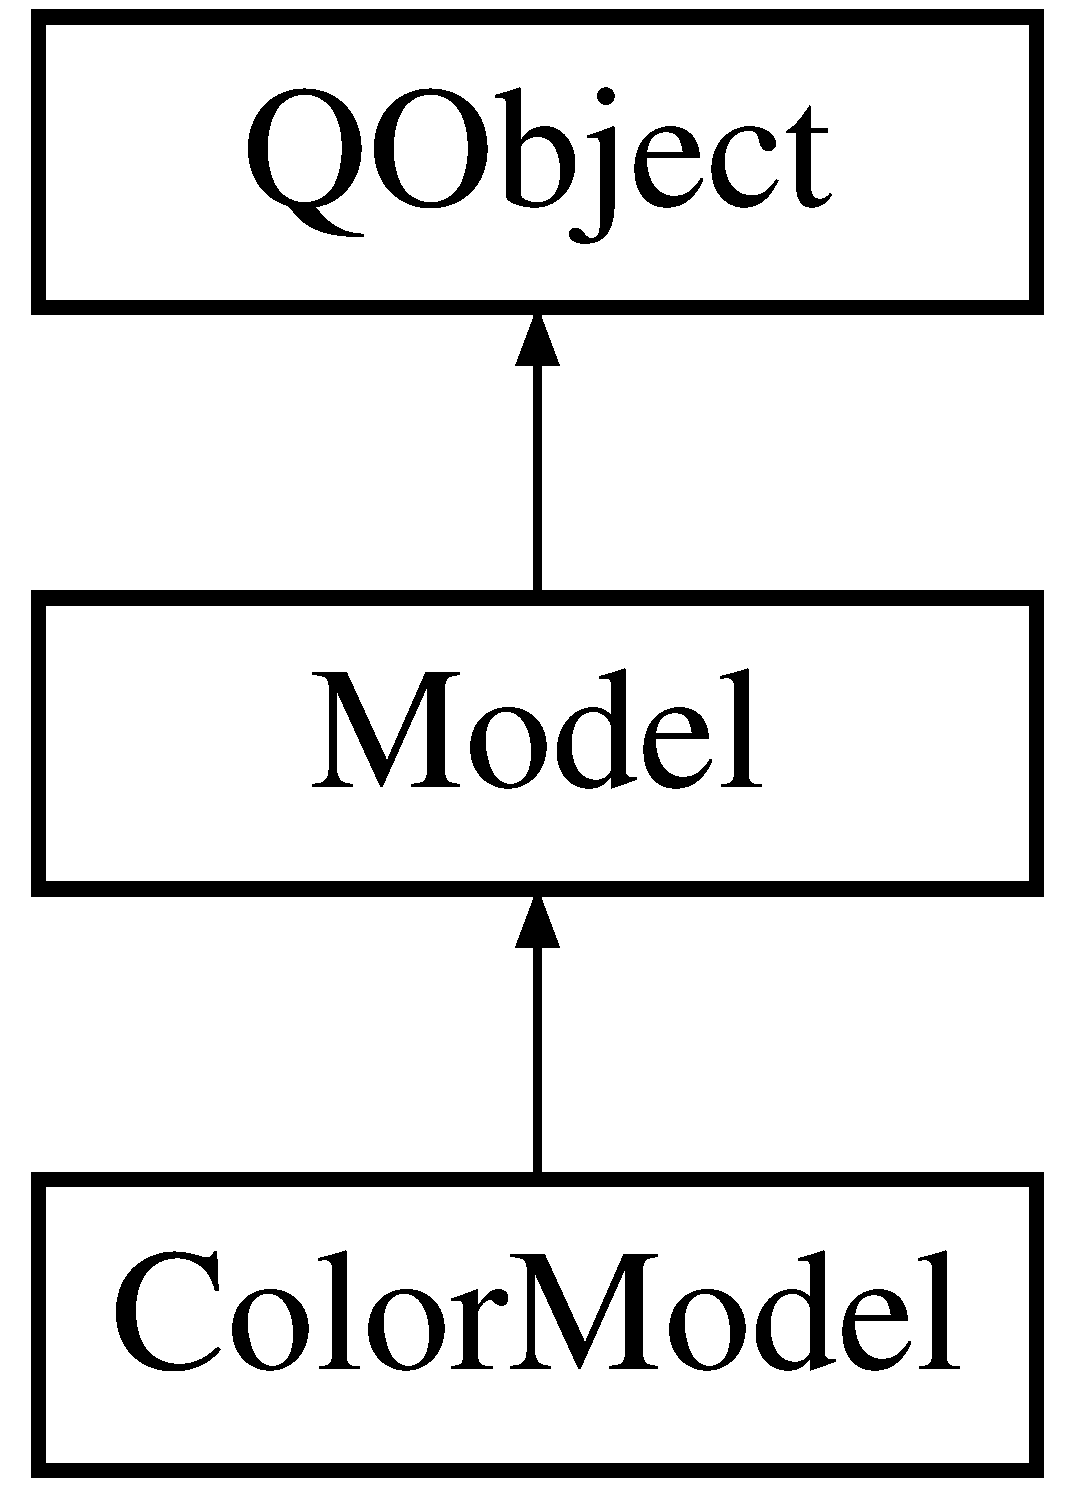
\includegraphics[height=3.000000cm]{class_model}
\end{center}
\end{figure}
\subsection*{Public Slots}
\begin{DoxyCompactItemize}
\item 
\mbox{\Hypertarget{class_model_a61d4e70e34d66e77bd508016be6e9637}\label{class_model_a61d4e70e34d66e77bd508016be6e9637}} 
virtual void {\bfseries set\+Left\+Type} (Q\+String type)=0
\item 
\mbox{\Hypertarget{class_model_ac3c03d44daacd6ad697481c576596592}\label{class_model_ac3c03d44daacd6ad697481c576596592}} 
virtual void {\bfseries set\+Left\+Values} (Q\+Vector$<$ Q\+String $>$ values)=0
\item 
\mbox{\Hypertarget{class_model_a967c3fccc96188c8087b1062045af857}\label{class_model_a967c3fccc96188c8087b1062045af857}} 
virtual void {\bfseries set\+Right\+Type} (Q\+String type)=0
\item 
\mbox{\Hypertarget{class_model_aed3bb530900e322630e2e39eb780991f}\label{class_model_aed3bb530900e322630e2e39eb780991f}} 
virtual void {\bfseries set\+Right\+Values} (Q\+Vector$<$ Q\+String $>$ values)=0
\item 
\mbox{\Hypertarget{class_model_aac934ac17dd66822dbbc074c2d8808b5}\label{class_model_aac934ac17dd66822dbbc074c2d8808b5}} 
virtual void {\bfseries set\+Result\+Type} (Q\+String type)=0
\item 
\mbox{\Hypertarget{class_model_ac58ba62771e20dd87da313b7e399df69}\label{class_model_ac58ba62771e20dd87da313b7e399df69}} 
virtual void {\bfseries set\+Op} (Q\+String e\+Operation)=0
\item 
\mbox{\Hypertarget{class_model_a95509d1e8dd8acff059eec72ac75f496}\label{class_model_a95509d1e8dd8acff059eec72ac75f496}} 
virtual void {\bfseries execute} ()=0
\item 
\mbox{\Hypertarget{class_model_a00ecb7bd9d19ba145a1ec536539fe08f}\label{class_model_a00ecb7bd9d19ba145a1ec536539fe08f}} 
virtual void {\bfseries get\+Result} ()=0
\item 
\mbox{\Hypertarget{class_model_a7328dea3602ce9c290c6821fba74cc6b}\label{class_model_a7328dea3602ce9c290c6821fba74cc6b}} 
virtual void {\bfseries get\+History} ()=0
\item 
\mbox{\Hypertarget{class_model_a6e2f20f21dccde450c3eb1b8eef3126b}\label{class_model_a6e2f20f21dccde450c3eb1b8eef3126b}} 
virtual void {\bfseries reset} ()=0
\end{DoxyCompactItemize}
\subsection*{Signals}
\begin{DoxyCompactItemize}
\item 
\mbox{\Hypertarget{class_model_a636cd0b310ee32bd0d7f4a158cb56b6d}\label{class_model_a636cd0b310ee32bd0d7f4a158cb56b6d}} 
void {\bfseries permitted\+Operations} (Q\+Vector$<$ Q\+String $>$ operations)
\item 
\mbox{\Hypertarget{class_model_a533d6dc0f4b7ed4d49f308b689a7747f}\label{class_model_a533d6dc0f4b7ed4d49f308b689a7747f}} 
void {\bfseries left\+Size} (int size, const Q\+Vector$<$ Q\+String $>$ \&limits)
\item 
\mbox{\Hypertarget{class_model_a640b1f4da464ee848601f9122dab5bc4}\label{class_model_a640b1f4da464ee848601f9122dab5bc4}} 
void {\bfseries right\+Size} (int size, const Q\+Vector$<$ Q\+String $>$ \&limits)
\item 
\mbox{\Hypertarget{class_model_a4019e969fe2996f955d07852f10693dd}\label{class_model_a4019e969fe2996f955d07852f10693dd}} 
void {\bfseries right\+Types} (Q\+Vector$<$ Q\+String $>$ permitted\+Types)
\item 
\mbox{\Hypertarget{class_model_a80434fb1d9e3abe82df328164a894e2f}\label{class_model_a80434fb1d9e3abe82df328164a894e2f}} 
void {\bfseries result\+Size} (int size)
\item 
\mbox{\Hypertarget{class_model_ae794cf24374d3c78f1b49731d096a077}\label{class_model_ae794cf24374d3c78f1b49731d096a077}} 
void {\bfseries result\+Ready} (Q\+Vector$<$ Q\+String $>$ result)
\item 
\mbox{\Hypertarget{class_model_a084ed959b9dbdac8f33047916a2b1e9e}\label{class_model_a084ed959b9dbdac8f33047916a2b1e9e}} 
void {\bfseries history} (const Q\+Vector$<$ Q\+Vector$<$ Q\+String $>$$>$ \&history\+Vector)
\item 
\mbox{\Hypertarget{class_model_a1bef8f3d9f6d483c016e3b8d30ea6025}\label{class_model_a1bef8f3d9f6d483c016e3b8d30ea6025}} 
void {\bfseries error} (Q\+String)
\item 
\mbox{\Hypertarget{class_model_aa06479997ae88278ab636dc302e1fb70}\label{class_model_aa06479997ae88278ab636dc302e1fb70}} 
void {\bfseries reset\+Type\+At} (Q\+String drop, Q\+String type)
\end{DoxyCompactItemize}
\subsection*{Public Member Functions}
\begin{DoxyCompactItemize}
\item 
\mbox{\Hypertarget{class_model_a2e34231c9285a6c0a3e3f0c5cd4d51aa}\label{class_model_a2e34231c9285a6c0a3e3f0c5cd4d51aa}} 
virtual Q\+Vector$<$ Q\+String $>$ {\bfseries available\+Operations} () const =0
\item 
\mbox{\Hypertarget{class_model_ad8efaa1708d2179e4a8e1474cae2df1d}\label{class_model_ad8efaa1708d2179e4a8e1474cae2df1d}} 
virtual Q\+Vector$<$ Q\+String $>$ {\bfseries all\+Available\+Types} () const =0
\end{DoxyCompactItemize}


\subsection{Detailed Description}
this abstract class is used by controller to be connected to the view 

The documentation for this class was generated from the following file\+:\begin{DoxyCompactItemize}
\item 
/home/gian/\+Projects/\+Kalk2-\/0/\+Kalk/\+Model/\hyperlink{model_8h}{model.\+h}\end{DoxyCompactItemize}

\hypertarget{class_r_g_b}{}\section{R\+GB Class Reference}
\label{class_r_g_b}\index{R\+GB@{R\+GB}}


this class uses the as base class \hyperlink{class_c_i_exyz}{C\+I\+Exyz} \hyperlink{class_r_g_b}{R\+GB} stores a color in \hyperlink{class_r_g_b}{R\+GB} representation  




{\ttfamily \#include $<$rgb.\+h$>$}

Inheritance diagram for R\+GB\+:\begin{figure}[H]
\begin{center}
\leavevmode
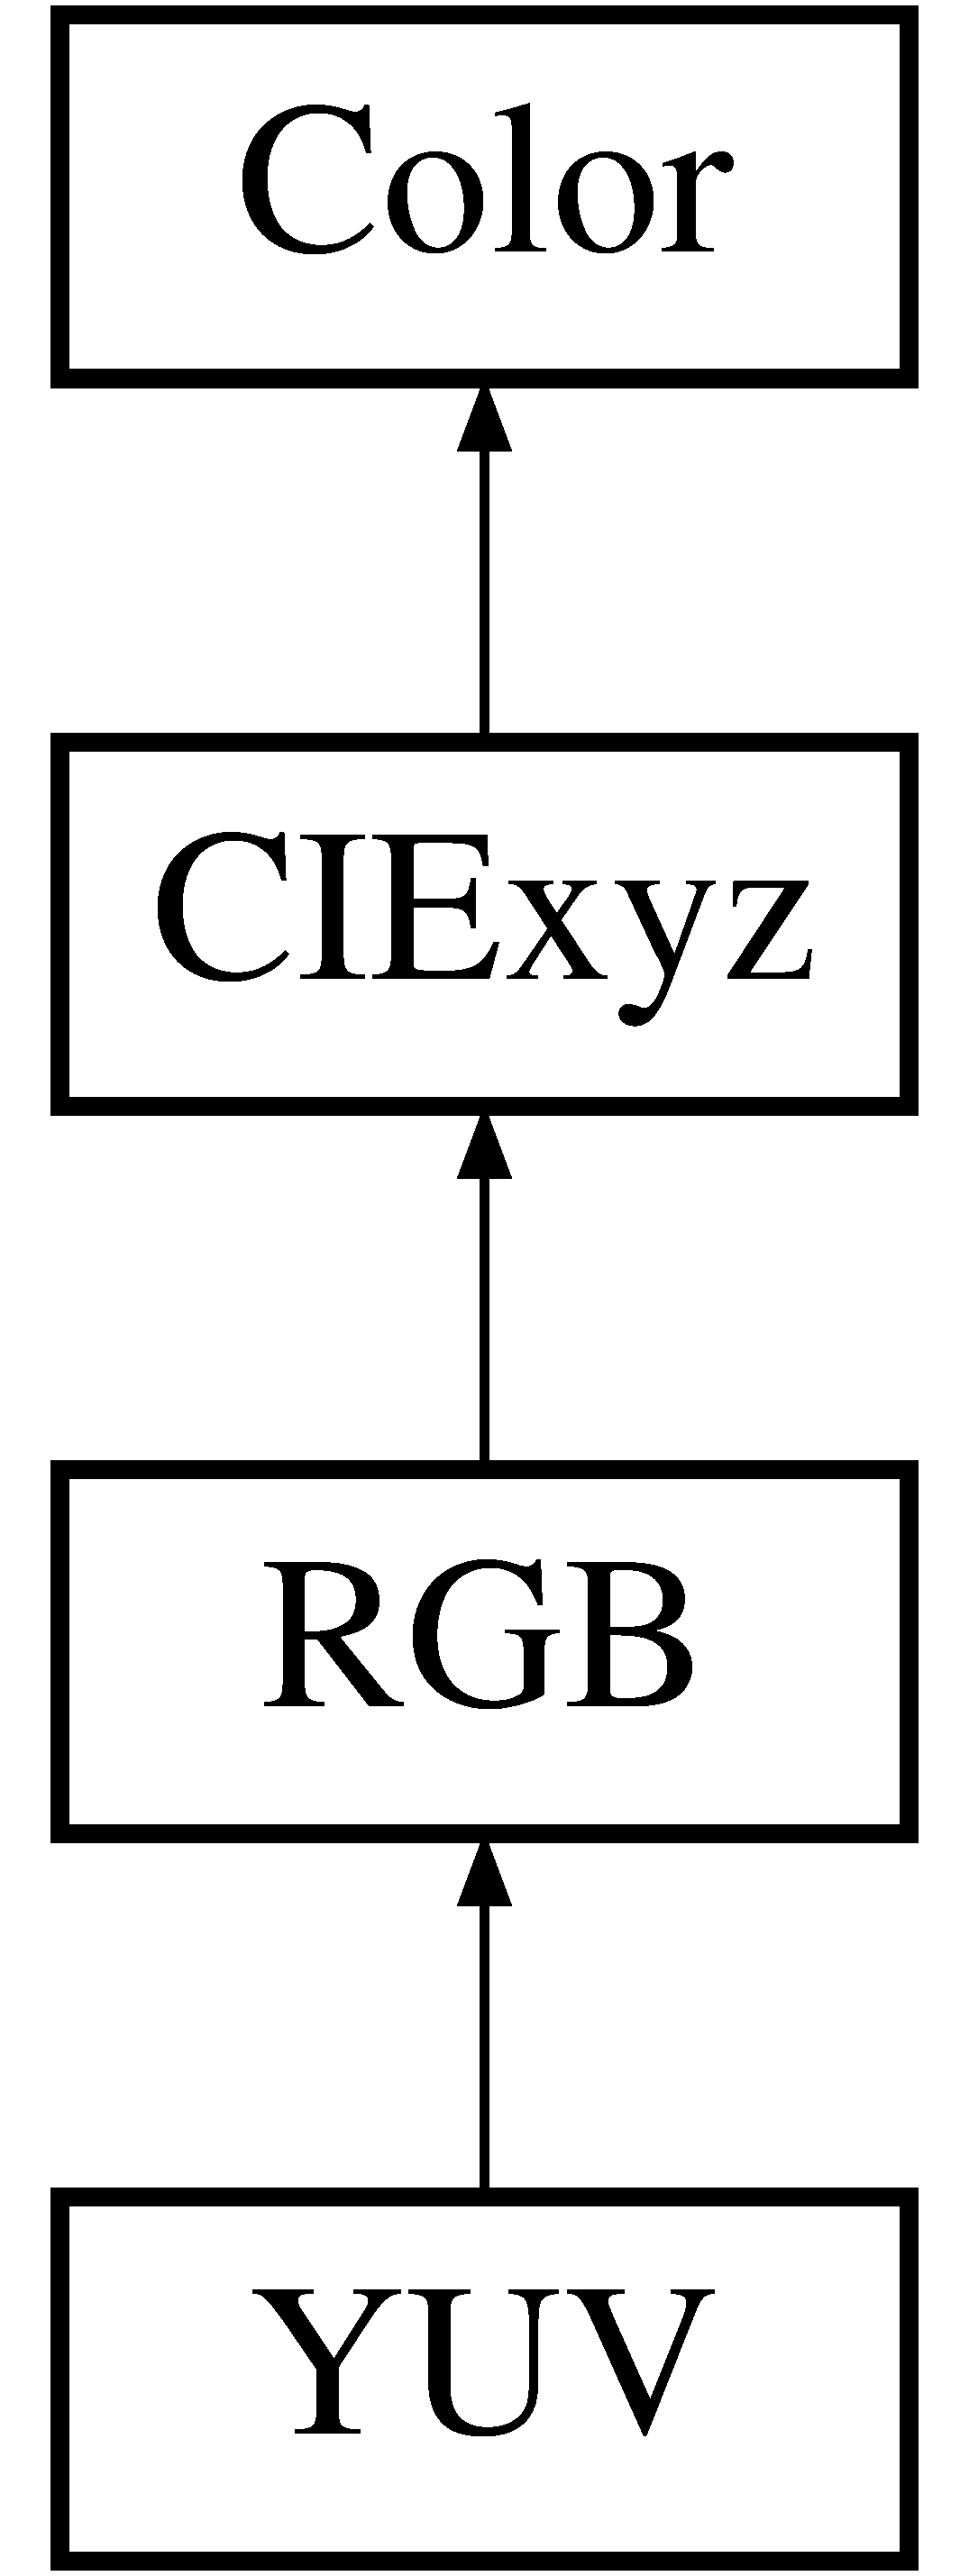
\includegraphics[height=4.000000cm]{class_r_g_b}
\end{center}
\end{figure}
\subsection*{Public Member Functions}
\begin{DoxyCompactItemize}
\item 
\hyperlink{class_r_g_b_ab48fc0751f6432ff993b31119f289001}{R\+GB} (int r=0, int g=0, int b=0)
\begin{DoxyCompactList}\small\item\em \hyperlink{class_r_g_b_ab48fc0751f6432ff993b31119f289001}{R\+G\+B\+::\+R\+GB}. \end{DoxyCompactList}\item 
\hyperlink{class_r_g_b_a4b69fccf264945ab5d708738824bd93a}{R\+GB} (const \hyperlink{class_r_g_b}{R\+GB} \&c)
\begin{DoxyCompactList}\small\item\em \hyperlink{class_r_g_b_ab48fc0751f6432ff993b31119f289001}{R\+G\+B\+::\+R\+GB}. \end{DoxyCompactList}\item 
\hyperlink{class_r_g_b_a9caf6caec9c6e67896b24ba3a1715342}{R\+GB} (const \hyperlink{class_r_g_b}{R\+GB} $\ast$c)
\begin{DoxyCompactList}\small\item\em \hyperlink{class_r_g_b_ab48fc0751f6432ff993b31119f289001}{R\+G\+B\+::\+R\+GB}. \end{DoxyCompactList}\item 
\hyperlink{class_r_g_b_acabd7e004d54445c5e87f27fcd06ad33}{R\+GB} (const \hyperlink{class_color}{Color} $\ast$c)
\begin{DoxyCompactList}\small\item\em \hyperlink{class_r_g_b_ab48fc0751f6432ff993b31119f289001}{R\+G\+B\+::\+R\+GB}. \end{DoxyCompactList}\item 
\hyperlink{class_color}{Color} $\ast$ \hyperlink{class_r_g_b_ac4b085d5587c664f7f9ceae1eb857d24}{get\+C\+IE} () const
\begin{DoxyCompactList}\small\item\em \hyperlink{class_r_g_b_ac4b085d5587c664f7f9ceae1eb857d24}{R\+G\+B\+::get\+C\+IE}. \end{DoxyCompactList}\item 
void \hyperlink{class_r_g_b_acf213178f2029a5f304d62b87dbb6b36}{set\+Components} (Q\+Vector$<$ double $>$ componets)
\begin{DoxyCompactList}\small\item\em \hyperlink{class_r_g_b_acf213178f2029a5f304d62b87dbb6b36}{R\+G\+B\+::set\+Components} set the components inside the object. \end{DoxyCompactList}\item 
Q\+String \hyperlink{class_r_g_b_a5f7a68904e1e4f18c22c1066170fb2bf}{get\+Representation} () const
\begin{DoxyCompactList}\small\item\em R\+G\+B\+::getrepresentation returns the meaning of the values contained in \hyperlink{class_r_g_b_ad085d3bd654d874ea2e5739a5c216769}{get\+Components()} \end{DoxyCompactList}\item 
\hyperlink{class_color}{Color} $\ast$ \hyperlink{class_r_g_b_a7aad38ac17ec3201c65f8f5e90637b69}{negate} () const
\begin{DoxyCompactList}\small\item\em \hyperlink{class_r_g_b_a7aad38ac17ec3201c65f8f5e90637b69}{R\+G\+B\+::negate}. \end{DoxyCompactList}\item 
\hyperlink{class_color}{Color} $\ast$ \hyperlink{class_r_g_b_aa022866e33474ab64f81d367c6b030b9}{mix} (const \hyperlink{class_color}{Color} $\ast$c) const
\begin{DoxyCompactList}\small\item\em \hyperlink{class_r_g_b_aa022866e33474ab64f81d367c6b030b9}{R\+G\+B\+::mix}. \end{DoxyCompactList}\item 
\hyperlink{class_color}{Color} $\ast$ \hyperlink{class_r_g_b_a9d250e0f58e7ae7d4c69ced724da6f80}{operator/} (const int \&div) const
\begin{DoxyCompactList}\small\item\em \hyperlink{class_r_g_b_a9d250e0f58e7ae7d4c69ced724da6f80}{R\+G\+B\+::operator /} new \hyperlink{class_r_g_b}{R\+GB} object with value divided. \end{DoxyCompactList}\item 
Q\+Vector$<$ Q\+String $>$ \hyperlink{class_r_g_b_a6cde5a9d00036c76fef2dd51ca8256a4}{available\+Operations} () const
\begin{DoxyCompactList}\small\item\em \hyperlink{class_r_g_b_a6cde5a9d00036c76fef2dd51ca8256a4}{R\+G\+B\+::available\+Operations} returns all the operation that has been implemented. \end{DoxyCompactList}\item 
Q\+Vector$<$ double $>$ \hyperlink{class_r_g_b_ad085d3bd654d874ea2e5739a5c216769}{get\+Components} () const
\begin{DoxyCompactList}\small\item\em \hyperlink{class_r_g_b_ad085d3bd654d874ea2e5739a5c216769}{R\+G\+B\+::get\+Components};. \end{DoxyCompactList}\item 
int \hyperlink{class_r_g_b_a7561d57d6706bc25ea10762d906b2345}{get\+Number\+Of\+Componets} () const
\begin{DoxyCompactList}\small\item\em \hyperlink{class_r_g_b_a7561d57d6706bc25ea10762d906b2345}{R\+G\+B\+::get\+Number\+Of\+Componets}. \end{DoxyCompactList}\item 
Q\+Vector$<$ Q\+String $>$ \hyperlink{class_r_g_b_a4ae8d5c061e45f557a5924f2237c1d0e}{get\+Limits} () const
\begin{DoxyCompactList}\small\item\em \hyperlink{class_r_g_b_a4ae8d5c061e45f557a5924f2237c1d0e}{R\+G\+B\+::get\+Limits}. \end{DoxyCompactList}\item 
\hyperlink{class_c_i_exyz}{C\+I\+Exyz} $\ast$ \hyperlink{class_r_g_b_a153f315167dfd89944c625d43b307b43}{get\+C\+IE} (int t\+\_\+r, int t\+\_\+g, int t\+\_\+b) const
\begin{DoxyCompactList}\small\item\em \hyperlink{class_r_g_b_ac4b085d5587c664f7f9ceae1eb857d24}{R\+G\+B\+::get\+C\+IE} converts \hyperlink{class_r_g_b}{R\+GB} value to \hyperlink{class_c_i_exyz}{C\+I\+Exyz}. \end{DoxyCompactList}\end{DoxyCompactItemize}
\subsection*{Additional Inherited Members}


\subsection{Detailed Description}
this class uses the as base class \hyperlink{class_c_i_exyz}{C\+I\+Exyz} \hyperlink{class_r_g_b}{R\+GB} stores a color in \hyperlink{class_r_g_b}{R\+GB} representation 

\subsection{Constructor \& Destructor Documentation}
\mbox{\Hypertarget{class_r_g_b_ab48fc0751f6432ff993b31119f289001}\label{class_r_g_b_ab48fc0751f6432ff993b31119f289001}} 
\index{R\+GB@{R\+GB}!R\+GB@{R\+GB}}
\index{R\+GB@{R\+GB}!R\+GB@{R\+GB}}
\subsubsection{\texorpdfstring{R\+G\+B()}{RGB()}\hspace{0.1cm}{\footnotesize\ttfamily [1/4]}}
{\footnotesize\ttfamily R\+G\+B\+::\+R\+GB (\begin{DoxyParamCaption}\item[{int}]{t\+\_\+r = {\ttfamily 0},  }\item[{int}]{t\+\_\+g = {\ttfamily 0},  }\item[{int}]{t\+\_\+b = {\ttfamily 0} }\end{DoxyParamCaption})}



\hyperlink{class_r_g_b_ab48fc0751f6432ff993b31119f289001}{R\+G\+B\+::\+R\+GB}. 


\begin{DoxyParams}{Parameters}
{\em int} & t\+\_\+r \\
\hline
{\em int} & t\+\_\+g \\
\hline
{\em int} & t\+\_\+b \\
\hline
\end{DoxyParams}

\begin{DoxyExceptions}{Exceptions}
{\em \hyperlink{class_illegal_color_exception}{Illegal\+Color\+Exception}} & uses the local function get\+C\+I\+E(int t\+\_\+r, int t\+\_\+g, int t\+\_\+b) to inizialize the parent object and set the local array values to rgb in input order \\
\hline
\end{DoxyExceptions}
\mbox{\Hypertarget{class_r_g_b_a4b69fccf264945ab5d708738824bd93a}\label{class_r_g_b_a4b69fccf264945ab5d708738824bd93a}} 
\index{R\+GB@{R\+GB}!R\+GB@{R\+GB}}
\index{R\+GB@{R\+GB}!R\+GB@{R\+GB}}
\subsubsection{\texorpdfstring{R\+G\+B()}{RGB()}\hspace{0.1cm}{\footnotesize\ttfamily [2/4]}}
{\footnotesize\ttfamily R\+G\+B\+::\+R\+GB (\begin{DoxyParamCaption}\item[{const \hyperlink{class_r_g_b}{R\+GB} \&}]{t\+\_\+c }\end{DoxyParamCaption})}



\hyperlink{class_r_g_b_ab48fc0751f6432ff993b31119f289001}{R\+G\+B\+::\+R\+GB}. 


\begin{DoxyParams}{Parameters}
{\em R\+G\+B\&} & t\+\_\+c Constructor that takes a \hyperlink{class_r_g_b}{R\+GB} pointer and clones the object \\
\hline
\end{DoxyParams}
\mbox{\Hypertarget{class_r_g_b_a9caf6caec9c6e67896b24ba3a1715342}\label{class_r_g_b_a9caf6caec9c6e67896b24ba3a1715342}} 
\index{R\+GB@{R\+GB}!R\+GB@{R\+GB}}
\index{R\+GB@{R\+GB}!R\+GB@{R\+GB}}
\subsubsection{\texorpdfstring{R\+G\+B()}{RGB()}\hspace{0.1cm}{\footnotesize\ttfamily [3/4]}}
{\footnotesize\ttfamily R\+G\+B\+::\+R\+GB (\begin{DoxyParamCaption}\item[{const \hyperlink{class_r_g_b}{R\+GB} $\ast$}]{t\+\_\+c }\end{DoxyParamCaption})}



\hyperlink{class_r_g_b_ab48fc0751f6432ff993b31119f289001}{R\+G\+B\+::\+R\+GB}. 


\begin{DoxyParams}{Parameters}
{\em R\+G\+B$\ast$} & t\+\_\+c \\
\hline
\end{DoxyParams}
\mbox{\Hypertarget{class_r_g_b_acabd7e004d54445c5e87f27fcd06ad33}\label{class_r_g_b_acabd7e004d54445c5e87f27fcd06ad33}} 
\index{R\+GB@{R\+GB}!R\+GB@{R\+GB}}
\index{R\+GB@{R\+GB}!R\+GB@{R\+GB}}
\subsubsection{\texorpdfstring{R\+G\+B()}{RGB()}\hspace{0.1cm}{\footnotesize\ttfamily [4/4]}}
{\footnotesize\ttfamily R\+G\+B\+::\+R\+GB (\begin{DoxyParamCaption}\item[{const \hyperlink{class_color}{Color} $\ast$}]{t\+\_\+c }\end{DoxyParamCaption})}



\hyperlink{class_r_g_b_ab48fc0751f6432ff993b31119f289001}{R\+G\+B\+::\+R\+GB}. 


\begin{DoxyParams}{Parameters}
{\em Color$\ast$} & t\+\_\+c Constructor for \hyperlink{class_r_g_b}{R\+GB} that get a \hyperlink{class_color}{Color} pointer And inzialize parent objcet with a clone of \hyperlink{class_c_i_exyz}{C\+I\+Exyz} representation \\
\hline
\end{DoxyParams}


\subsection{Member Function Documentation}
\mbox{\Hypertarget{class_r_g_b_a6cde5a9d00036c76fef2dd51ca8256a4}\label{class_r_g_b_a6cde5a9d00036c76fef2dd51ca8256a4}} 
\index{R\+GB@{R\+GB}!available\+Operations@{available\+Operations}}
\index{available\+Operations@{available\+Operations}!R\+GB@{R\+GB}}
\subsubsection{\texorpdfstring{available\+Operations()}{availableOperations()}}
{\footnotesize\ttfamily Q\+Vector$<$ Q\+String $>$ R\+G\+B\+::available\+Operations (\begin{DoxyParamCaption}{ }\end{DoxyParamCaption}) const\hspace{0.3cm}{\ttfamily [virtual]}}



\hyperlink{class_r_g_b_a6cde5a9d00036c76fef2dd51ca8256a4}{R\+G\+B\+::available\+Operations} returns all the operation that has been implemented. 

\begin{DoxyReturn}{Returns}
Q\+Vector$<$\+Q\+String$>$ 
\end{DoxyReturn}


Reimplemented from \hyperlink{class_c_i_exyz_aa82a27c78ff425e06cdd740dd50e93b1}{C\+I\+Exyz}.

\mbox{\Hypertarget{class_r_g_b_ac4b085d5587c664f7f9ceae1eb857d24}\label{class_r_g_b_ac4b085d5587c664f7f9ceae1eb857d24}} 
\index{R\+GB@{R\+GB}!get\+C\+IE@{get\+C\+IE}}
\index{get\+C\+IE@{get\+C\+IE}!R\+GB@{R\+GB}}
\subsubsection{\texorpdfstring{get\+C\+I\+E()}{getCIE()}\hspace{0.1cm}{\footnotesize\ttfamily [1/2]}}
{\footnotesize\ttfamily \hyperlink{class_color}{Color} $\ast$ R\+G\+B\+::get\+C\+IE (\begin{DoxyParamCaption}{ }\end{DoxyParamCaption}) const\hspace{0.3cm}{\ttfamily [virtual]}}



\hyperlink{class_r_g_b_ac4b085d5587c664f7f9ceae1eb857d24}{R\+G\+B\+::get\+C\+IE}. 

\begin{DoxyReturn}{Returns}
a new \hyperlink{class_color}{Color} object as \hyperlink{class_c_i_exyz}{C\+I\+Exyz} 
\end{DoxyReturn}


Reimplemented from \hyperlink{class_c_i_exyz_aa93c7a293b63c7bce8d1fab9a185ab1b}{C\+I\+Exyz}.

\mbox{\Hypertarget{class_r_g_b_a153f315167dfd89944c625d43b307b43}\label{class_r_g_b_a153f315167dfd89944c625d43b307b43}} 
\index{R\+GB@{R\+GB}!get\+C\+IE@{get\+C\+IE}}
\index{get\+C\+IE@{get\+C\+IE}!R\+GB@{R\+GB}}
\subsubsection{\texorpdfstring{get\+C\+I\+E()}{getCIE()}\hspace{0.1cm}{\footnotesize\ttfamily [2/2]}}
{\footnotesize\ttfamily \hyperlink{class_c_i_exyz}{C\+I\+Exyz} $\ast$ R\+G\+B\+::get\+C\+IE (\begin{DoxyParamCaption}\item[{int}]{t\+\_\+r,  }\item[{int}]{t\+\_\+g,  }\item[{int}]{t\+\_\+b }\end{DoxyParamCaption}) const}



\hyperlink{class_r_g_b_ac4b085d5587c664f7f9ceae1eb857d24}{R\+G\+B\+::get\+C\+IE} converts \hyperlink{class_r_g_b}{R\+GB} value to \hyperlink{class_c_i_exyz}{C\+I\+Exyz}. 


\begin{DoxyParams}{Parameters}
{\em int} & t\+\_\+r \\
\hline
{\em int} & t\+\_\+g \\
\hline
{\em int} & t\+\_\+b \\
\hline
\end{DoxyParams}
\begin{DoxyReturn}{Returns}
a new \hyperlink{class_color}{Color} object as C\+I\+Exyz$\ast$ 
\end{DoxyReturn}
\mbox{\Hypertarget{class_r_g_b_ad085d3bd654d874ea2e5739a5c216769}\label{class_r_g_b_ad085d3bd654d874ea2e5739a5c216769}} 
\index{R\+GB@{R\+GB}!get\+Components@{get\+Components}}
\index{get\+Components@{get\+Components}!R\+GB@{R\+GB}}
\subsubsection{\texorpdfstring{get\+Components()}{getComponents()}}
{\footnotesize\ttfamily Q\+Vector$<$ double $>$ R\+G\+B\+::get\+Components (\begin{DoxyParamCaption}{ }\end{DoxyParamCaption}) const\hspace{0.3cm}{\ttfamily [virtual]}}



\hyperlink{class_r_g_b_ad085d3bd654d874ea2e5739a5c216769}{R\+G\+B\+::get\+Components};. 

\begin{DoxyReturn}{Returns}
components in a Q\+Vector$<$double$>$ 
\end{DoxyReturn}


Reimplemented from \hyperlink{class_c_i_exyz_af8992e3ac1741c35fcb18aa2cdb554a0}{C\+I\+Exyz}.



Reimplemented in \hyperlink{class_y_u_v_ad90109db3486e61e248e274a7690824a}{Y\+UV}.

\mbox{\Hypertarget{class_r_g_b_a4ae8d5c061e45f557a5924f2237c1d0e}\label{class_r_g_b_a4ae8d5c061e45f557a5924f2237c1d0e}} 
\index{R\+GB@{R\+GB}!get\+Limits@{get\+Limits}}
\index{get\+Limits@{get\+Limits}!R\+GB@{R\+GB}}
\subsubsection{\texorpdfstring{get\+Limits()}{getLimits()}}
{\footnotesize\ttfamily Q\+Vector$<$ Q\+String $>$ R\+G\+B\+::get\+Limits (\begin{DoxyParamCaption}{ }\end{DoxyParamCaption}) const\hspace{0.3cm}{\ttfamily [virtual]}}



\hyperlink{class_r_g_b_a4ae8d5c061e45f557a5924f2237c1d0e}{R\+G\+B\+::get\+Limits}. 

\begin{DoxyReturn}{Returns}
\hyperlink{class_r_g_b}{R\+GB} limits as Q\+Vector$<$\+Q\+String$>$ 
\end{DoxyReturn}


Reimplemented from \hyperlink{class_c_i_exyz_a4c3aa6777f7720ae26b53174322a83f8}{C\+I\+Exyz}.



Reimplemented in \hyperlink{class_y_u_v_a344cd573b663c97f5554afcb1c15458c}{Y\+UV}.

\mbox{\Hypertarget{class_r_g_b_a7561d57d6706bc25ea10762d906b2345}\label{class_r_g_b_a7561d57d6706bc25ea10762d906b2345}} 
\index{R\+GB@{R\+GB}!get\+Number\+Of\+Componets@{get\+Number\+Of\+Componets}}
\index{get\+Number\+Of\+Componets@{get\+Number\+Of\+Componets}!R\+GB@{R\+GB}}
\subsubsection{\texorpdfstring{get\+Number\+Of\+Componets()}{getNumberOfComponets()}}
{\footnotesize\ttfamily int R\+G\+B\+::get\+Number\+Of\+Componets (\begin{DoxyParamCaption}{ }\end{DoxyParamCaption}) const\hspace{0.3cm}{\ttfamily [virtual]}}



\hyperlink{class_r_g_b_a7561d57d6706bc25ea10762d906b2345}{R\+G\+B\+::get\+Number\+Of\+Componets}. 

\begin{DoxyReturn}{Returns}
int 
\end{DoxyReturn}


Reimplemented from \hyperlink{class_c_i_exyz_af168733bb1bca36a7ae5d75c67de046e}{C\+I\+Exyz}.



Reimplemented in \hyperlink{class_y_u_v_a46eded5c13a0c2b2e9bbf05d4a2f9c7c}{Y\+UV}.

\mbox{\Hypertarget{class_r_g_b_a5f7a68904e1e4f18c22c1066170fb2bf}\label{class_r_g_b_a5f7a68904e1e4f18c22c1066170fb2bf}} 
\index{R\+GB@{R\+GB}!get\+Representation@{get\+Representation}}
\index{get\+Representation@{get\+Representation}!R\+GB@{R\+GB}}
\subsubsection{\texorpdfstring{get\+Representation()}{getRepresentation()}}
{\footnotesize\ttfamily Q\+String R\+G\+B\+::get\+Representation (\begin{DoxyParamCaption}{ }\end{DoxyParamCaption}) const\hspace{0.3cm}{\ttfamily [virtual]}}



R\+G\+B\+::getrepresentation returns the meaning of the values contained in \hyperlink{class_r_g_b_ad085d3bd654d874ea2e5739a5c216769}{get\+Components()} 

\begin{DoxyReturn}{Returns}
Q\+String that contains name of the object 
\end{DoxyReturn}


Reimplemented from \hyperlink{class_c_i_exyz_a19120c15d1304696909d76fae6065ebd}{C\+I\+Exyz}.



Reimplemented in \hyperlink{class_y_u_v_ae38403ffd397003eb28ab7670f95d1e5}{Y\+UV}.

\mbox{\Hypertarget{class_r_g_b_aa022866e33474ab64f81d367c6b030b9}\label{class_r_g_b_aa022866e33474ab64f81d367c6b030b9}} 
\index{R\+GB@{R\+GB}!mix@{mix}}
\index{mix@{mix}!R\+GB@{R\+GB}}
\subsubsection{\texorpdfstring{mix()}{mix()}}
{\footnotesize\ttfamily \hyperlink{class_color}{Color} $\ast$ R\+G\+B\+::mix (\begin{DoxyParamCaption}\item[{const \hyperlink{class_color}{Color} $\ast$}]{t\+\_\+c }\end{DoxyParamCaption}) const\hspace{0.3cm}{\ttfamily [virtual]}}



\hyperlink{class_r_g_b_aa022866e33474ab64f81d367c6b030b9}{R\+G\+B\+::mix}. 


\begin{DoxyParams}{Parameters}
{\em Color$\ast$} & t\+\_\+c \\
\hline
\end{DoxyParams}
\begin{DoxyReturn}{Returns}
a new \hyperlink{class_color}{Color} object with the mixed Colors as \hyperlink{class_r_g_b}{R\+GB} 
\end{DoxyReturn}


Reimplemented from \hyperlink{class_c_i_exyz_af8eeb48ade44beea43d023b36d263fc8}{C\+I\+Exyz}.



Reimplemented in \hyperlink{class_y_u_v_ab152a4ea37eaa67df0b38882c2099da3}{Y\+UV}.

\mbox{\Hypertarget{class_r_g_b_a7aad38ac17ec3201c65f8f5e90637b69}\label{class_r_g_b_a7aad38ac17ec3201c65f8f5e90637b69}} 
\index{R\+GB@{R\+GB}!negate@{negate}}
\index{negate@{negate}!R\+GB@{R\+GB}}
\subsubsection{\texorpdfstring{negate()}{negate()}}
{\footnotesize\ttfamily \hyperlink{class_color}{Color} $\ast$ R\+G\+B\+::negate (\begin{DoxyParamCaption}{ }\end{DoxyParamCaption}) const\hspace{0.3cm}{\ttfamily [virtual]}}



\hyperlink{class_r_g_b_a7aad38ac17ec3201c65f8f5e90637b69}{R\+G\+B\+::negate}. 

\begin{DoxyReturn}{Returns}
return a new \hyperlink{class_color}{Color} object with a new negated color as \hyperlink{class_r_g_b}{R\+GB} 
\end{DoxyReturn}


Reimplemented from \hyperlink{class_c_i_exyz_a4a454df6cbb71f3fcfd2d1ea9d500d94}{C\+I\+Exyz}.



Reimplemented in \hyperlink{class_y_u_v_a079872ae88552066ce1abb39cc0a40de}{Y\+UV}.

\mbox{\Hypertarget{class_r_g_b_a9d250e0f58e7ae7d4c69ced724da6f80}\label{class_r_g_b_a9d250e0f58e7ae7d4c69ced724da6f80}} 
\index{R\+GB@{R\+GB}!operator/@{operator/}}
\index{operator/@{operator/}!R\+GB@{R\+GB}}
\subsubsection{\texorpdfstring{operator/()}{operator/()}}
{\footnotesize\ttfamily \hyperlink{class_color}{Color} $\ast$ R\+G\+B\+::operator/ (\begin{DoxyParamCaption}\item[{const int \&}]{div }\end{DoxyParamCaption}) const\hspace{0.3cm}{\ttfamily [virtual]}}



\hyperlink{class_r_g_b_a9d250e0f58e7ae7d4c69ced724da6f80}{R\+G\+B\+::operator /} new \hyperlink{class_r_g_b}{R\+GB} object with value divided. 


\begin{DoxyParams}{Parameters}
{\em int} & div \\
\hline
\end{DoxyParams}

\begin{DoxyExceptions}{Exceptions}
{\em \hyperlink{class_illegal_color_exception}{Illegal\+Color\+Exception}} & \\
\hline
\end{DoxyExceptions}
\begin{DoxyReturn}{Returns}
\hyperlink{class_r_g_b}{R\+GB} 
\end{DoxyReturn}


Reimplemented from \hyperlink{class_c_i_exyz_abb3f5e1c8a923d7758e6bbe83b71f4fa}{C\+I\+Exyz}.



Reimplemented in \hyperlink{class_y_u_v_a1b9300c00323eca16fc4bb028964e85f}{Y\+UV}.

\mbox{\Hypertarget{class_r_g_b_acf213178f2029a5f304d62b87dbb6b36}\label{class_r_g_b_acf213178f2029a5f304d62b87dbb6b36}} 
\index{R\+GB@{R\+GB}!set\+Components@{set\+Components}}
\index{set\+Components@{set\+Components}!R\+GB@{R\+GB}}
\subsubsection{\texorpdfstring{set\+Components()}{setComponents()}}
{\footnotesize\ttfamily void R\+G\+B\+::set\+Components (\begin{DoxyParamCaption}\item[{Q\+Vector$<$ double $>$}]{componets }\end{DoxyParamCaption})\hspace{0.3cm}{\ttfamily [virtual]}}



\hyperlink{class_r_g_b_acf213178f2029a5f304d62b87dbb6b36}{R\+G\+B\+::set\+Components} set the components inside the object. 


\begin{DoxyExceptions}{Exceptions}
{\em \hyperlink{class_illegal_color_exception}{Illegal\+Color\+Exception}} & \\
\hline
\end{DoxyExceptions}

\begin{DoxyParams}{Parameters}
{\em componets} & \\
\hline
\end{DoxyParams}


Reimplemented from \hyperlink{class_c_i_exyz_a11468574f91d2cb1356f0cde56429b84}{C\+I\+Exyz}.



Reimplemented in \hyperlink{class_y_u_v_a622daf7a688da4a227b63deb412c0d46}{Y\+UV}.



The documentation for this class was generated from the following files\+:\begin{DoxyCompactItemize}
\item 
/home/gian/\+Projects/\+Kalk2-\/0/\+Kalk/\+Model/\+Color/\+R\+G\+B/\hyperlink{rgb_8h}{rgb.\+h}\item 
/home/gian/\+Projects/\+Kalk2-\/0/\+Kalk/\+Model/\+Color/\+R\+G\+B/rgb.\+cpp\end{DoxyCompactItemize}

\hypertarget{class_view}{}\section{View Class Reference}
\label{class_view}\index{View@{View}}
Inheritance diagram for View\+:\begin{figure}[H]
\begin{center}
\leavevmode
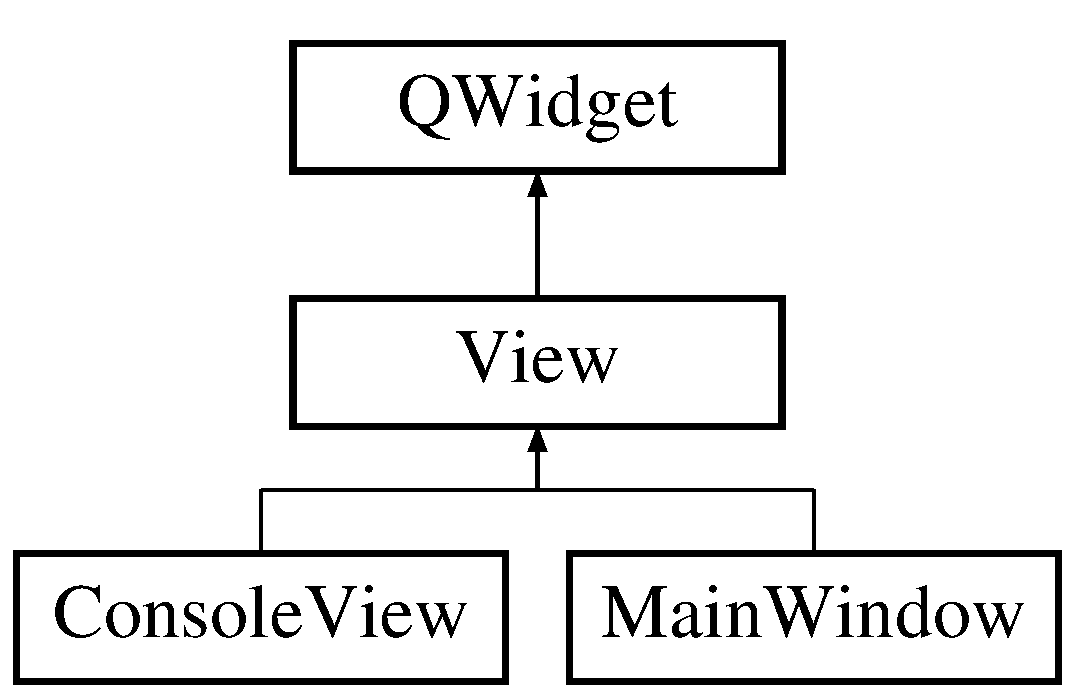
\includegraphics[height=3.000000cm]{class_view}
\end{center}
\end{figure}
\subsection*{Public Slots}
\begin{DoxyCompactItemize}
\item 
\mbox{\Hypertarget{class_view_a203ab36b8546f1d9dc630bd7c0536e67}\label{class_view_a203ab36b8546f1d9dc630bd7c0536e67}} 
virtual void {\bfseries set\+Available\+Operations} (const Q\+Vector$<$ Q\+String $>$ operations)=0
\item 
\mbox{\Hypertarget{class_view_a5b3c08e11f2aece6c28c9b36e41ae35a}\label{class_view_a5b3c08e11f2aece6c28c9b36e41ae35a}} 
virtual void {\bfseries set\+Permitted\+Operations} (const Q\+Vector$<$ Q\+String $>$ operations)=0
\item 
\mbox{\Hypertarget{class_view_a80c90f9167a8bc834d8c2f25be9e5f0d}\label{class_view_a80c90f9167a8bc834d8c2f25be9e5f0d}} 
virtual void {\bfseries set\+Left\+Types} (const Q\+Vector$<$ Q\+String $>$ types)=0
\item 
\mbox{\Hypertarget{class_view_a497493954a4a2be8cf50306a884d7358}\label{class_view_a497493954a4a2be8cf50306a884d7358}} 
virtual void {\bfseries set\+Left\+Fields} (const int \&fields, const Q\+Vector$<$ Q\+String $>$ \&limits)=0
\item 
\mbox{\Hypertarget{class_view_a26bb1996d32f29476ba3c0b5c01561fc}\label{class_view_a26bb1996d32f29476ba3c0b5c01561fc}} 
virtual void {\bfseries set\+Right\+Types} (const Q\+Vector$<$ Q\+String $>$ types)=0
\item 
\mbox{\Hypertarget{class_view_a342210db03ff75bfe4b66f3383e50341}\label{class_view_a342210db03ff75bfe4b66f3383e50341}} 
virtual void {\bfseries set\+Right\+Fields} (const int \&fields, const Q\+Vector$<$ Q\+String $>$ \&limits)=0
\item 
\mbox{\Hypertarget{class_view_a2d78db2bd23a6dd80bfeae64f4c3fdd3}\label{class_view_a2d78db2bd23a6dd80bfeae64f4c3fdd3}} 
virtual void {\bfseries set\+Result} (const Q\+Vector$<$ Q\+String $>$ result)=0
\item 
\mbox{\Hypertarget{class_view_ad3f5b700bd33a72bebc6efdbad2d17eb}\label{class_view_ad3f5b700bd33a72bebc6efdbad2d17eb}} 
virtual void {\bfseries set\+Result\+Fields} (const int \&fields)=0
\item 
\mbox{\Hypertarget{class_view_a3d017128dbceb8a10e0c35fcd852e987}\label{class_view_a3d017128dbceb8a10e0c35fcd852e987}} 
virtual void {\bfseries set\+History} (const Q\+Vector$<$ Q\+Vector$<$ Q\+String $>$$>$ \&history)=0
\item 
\mbox{\Hypertarget{class_view_a117a5d1b3b3e3823e628d859f6f3cb48}\label{class_view_a117a5d1b3b3e3823e628d859f6f3cb48}} 
virtual void {\bfseries error} (const Q\+String \&error\+\_\+message)=0
\item 
\mbox{\Hypertarget{class_view_a0fd83f152fae6bbcaf6537f4379fd15b}\label{class_view_a0fd83f152fae6bbcaf6537f4379fd15b}} 
virtual void {\bfseries reset\+Type} (Q\+String drop, Q\+String type)=0
\item 
\mbox{\Hypertarget{class_view_a913b840fc8042436555b89878feacb76}\label{class_view_a913b840fc8042436555b89878feacb76}} 
virtual void {\bfseries show} ()=0
\end{DoxyCompactItemize}
\subsection*{Signals}
\begin{DoxyCompactItemize}
\item 
\mbox{\Hypertarget{class_view_a96f2fd0ed3467a0e5072e9a4a5593395}\label{class_view_a96f2fd0ed3467a0e5072e9a4a5593395}} 
void {\bfseries left\+Values\+Are\+Set} (Q\+Vector$<$ Q\+String $>$ values)
\item 
\mbox{\Hypertarget{class_view_aef26164c727b9a1b83ca0e84c00a0060}\label{class_view_aef26164c727b9a1b83ca0e84c00a0060}} 
void {\bfseries right\+Values\+Are\+Set} (Q\+Vector$<$ Q\+String $>$ values)
\item 
\mbox{\Hypertarget{class_view_ae0775d09884cd6b001829df4276e407c}\label{class_view_ae0775d09884cd6b001829df4276e407c}} 
void {\bfseries left\+Type\+Is\+Set} (Q\+String type)
\item 
\mbox{\Hypertarget{class_view_a29e8b493fdbca2747da4ffa855ab966c}\label{class_view_a29e8b493fdbca2747da4ffa855ab966c}} 
void {\bfseries right\+Type\+Is\+Set} (Q\+String type)
\item 
\mbox{\Hypertarget{class_view_aa510baf4ace905a146c2655ca4a4b55e}\label{class_view_aa510baf4ace905a146c2655ca4a4b55e}} 
void {\bfseries result\+Type\+Is\+Set} (Q\+String type)
\item 
\mbox{\Hypertarget{class_view_af4cf1863986a0fac18d6da46c97329de}\label{class_view_af4cf1863986a0fac18d6da46c97329de}} 
void {\bfseries operation\+Is\+Set} (Q\+String opt)
\item 
\mbox{\Hypertarget{class_view_ac05f93e75953488aa1a5a3f813603032}\label{class_view_ac05f93e75953488aa1a5a3f813603032}} 
void {\bfseries get\+Result} ()
\item 
\mbox{\Hypertarget{class_view_a0cf275613b9eb5cc57e2069df61a87e1}\label{class_view_a0cf275613b9eb5cc57e2069df61a87e1}} 
void {\bfseries get\+History} ()
\item 
\mbox{\Hypertarget{class_view_a84eea48d2036da09640369d7997d957b}\label{class_view_a84eea48d2036da09640369d7997d957b}} 
void {\bfseries reset} ()
\item 
\mbox{\Hypertarget{class_view_af0a5104e717bfe94ae35a1dfd9d5e183}\label{class_view_af0a5104e717bfe94ae35a1dfd9d5e183}} 
void {\bfseries done} ()
\end{DoxyCompactItemize}
\subsection*{Public Member Functions}
\begin{DoxyCompactItemize}
\item 
\mbox{\Hypertarget{class_view_a3fd5b2cd3d7ccfc51dd4b2730833180c}\label{class_view_a3fd5b2cd3d7ccfc51dd4b2730833180c}} 
{\bfseries View} (Q\+Widget $\ast$parent=nullptr)
\end{DoxyCompactItemize}


The documentation for this class was generated from the following file\+:\begin{DoxyCompactItemize}
\item 
/home/gian/\+Projects/\+Kalk2-\/0/\+Kalk/\+View/\hyperlink{view_8h}{view.\+h}\end{DoxyCompactItemize}

\hypertarget{class_y_u_v}{}\section{Y\+UV Class Reference}
\label{class_y_u_v}\index{Y\+UV@{Y\+UV}}


this class uses as base the class \hyperlink{class_r_g_b}{R\+GB} \hyperlink{class_y_u_v}{Y\+UV} stores a color in \hyperlink{class_y_u_v}{Y\+UV} representation  




{\ttfamily \#include $<$yuv.\+h$>$}

Inheritance diagram for Y\+UV\+:\begin{figure}[H]
\begin{center}
\leavevmode
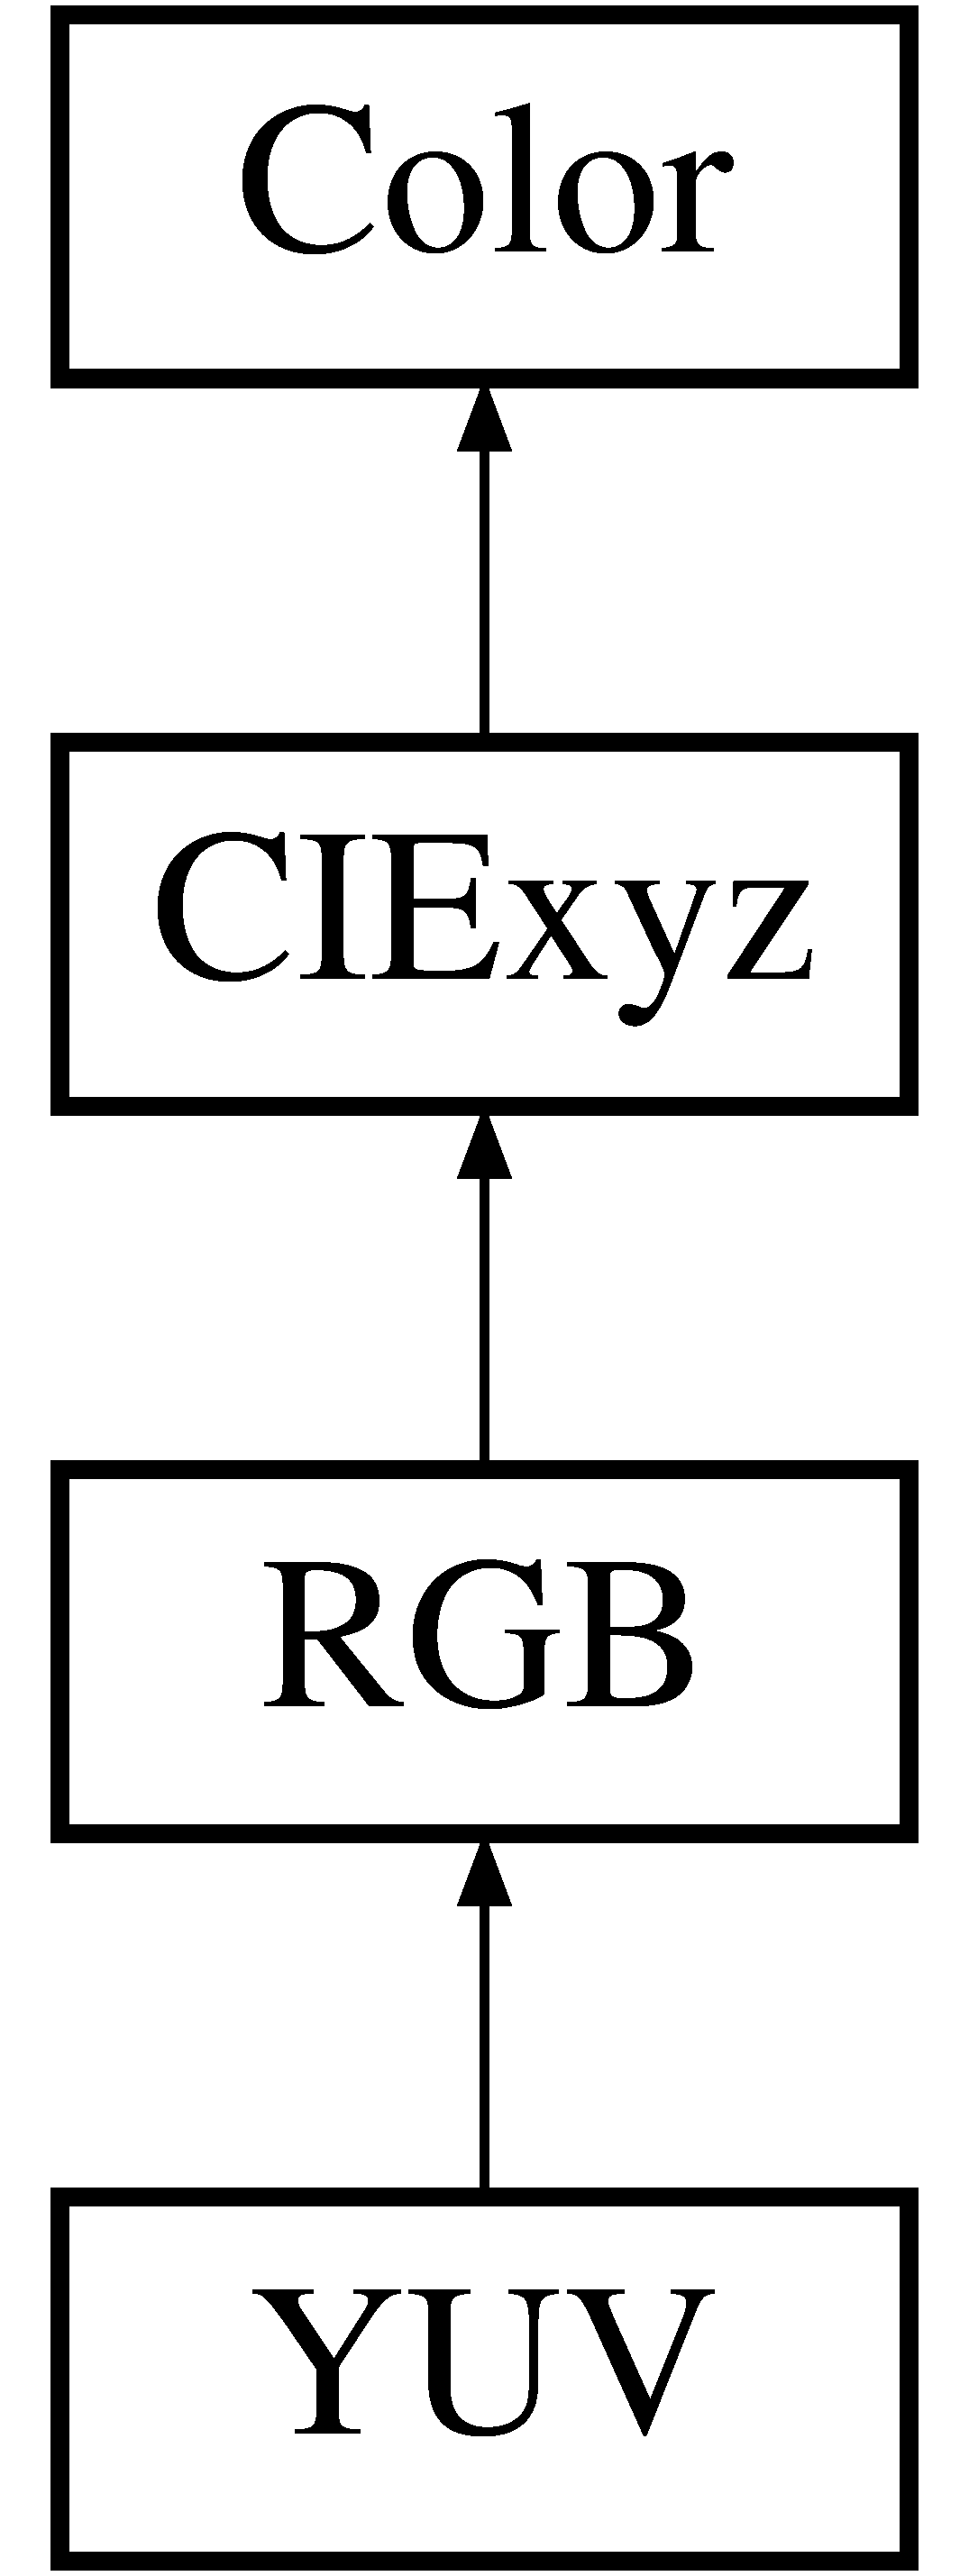
\includegraphics[height=4.000000cm]{class_y_u_v}
\end{center}
\end{figure}
\subsection*{Public Member Functions}
\begin{DoxyCompactItemize}
\item 
\hyperlink{class_y_u_v_aafa9b0e5ddae51a501c13c9c4b106b84}{Y\+UV} (double \+\_\+y=0, double \+\_\+u=0, double \+\_\+v=0)
\begin{DoxyCompactList}\small\item\em \hyperlink{class_y_u_v_aafa9b0e5ddae51a501c13c9c4b106b84}{Y\+U\+V\+::\+Y\+UV} Constructor for \hyperlink{class_y_u_v}{Y\+UV} color representation from double precision numbers. \end{DoxyCompactList}\item 
\hyperlink{class_y_u_v_a80778948bf90243f1424e06f9dfbbbf1}{Y\+UV} (const \hyperlink{class_color}{Color} $\ast$from)
\begin{DoxyCompactList}\small\item\em \hyperlink{class_y_u_v_aafa9b0e5ddae51a501c13c9c4b106b84}{Y\+U\+V\+::\+Y\+UV} Constructor for \hyperlink{class_y_u_v}{Y\+UV} color representation from \hyperlink{class_color}{Color} pointer. \end{DoxyCompactList}\item 
\hyperlink{class_y_u_v_af6de31964471999a64e34af00ef6e196}{Y\+UV} (const \hyperlink{class_y_u_v}{Y\+UV} \&from)
\begin{DoxyCompactList}\small\item\em \hyperlink{class_y_u_v_aafa9b0e5ddae51a501c13c9c4b106b84}{Y\+U\+V\+::\+Y\+UV} copy constructor. \end{DoxyCompactList}\item 
Q\+String \hyperlink{class_y_u_v_ae38403ffd397003eb28ab7670f95d1e5}{get\+Representation} () const
\begin{DoxyCompactList}\small\item\em Y\+U\+V\+::getrepresentation. \end{DoxyCompactList}\item 
\hyperlink{class_color}{Color} $\ast$ \hyperlink{class_y_u_v_a079872ae88552066ce1abb39cc0a40de}{negate} () const
\begin{DoxyCompactList}\small\item\em \hyperlink{class_y_u_v_a079872ae88552066ce1abb39cc0a40de}{Y\+U\+V\+::negate}. \end{DoxyCompactList}\item 
\hyperlink{class_color}{Color} $\ast$ \hyperlink{class_y_u_v_ab152a4ea37eaa67df0b38882c2099da3}{mix} (const \hyperlink{class_color}{Color} $\ast$a) const
\begin{DoxyCompactList}\small\item\em \hyperlink{class_y_u_v_ab152a4ea37eaa67df0b38882c2099da3}{Y\+U\+V\+::mix}. \end{DoxyCompactList}\item 
\hyperlink{class_color}{Color} $\ast$ \hyperlink{class_y_u_v_a56f11c27f1659c30ebd20c929704e004}{get\+C\+IE} (double y, double u, double v)
\begin{DoxyCompactList}\small\item\em \hyperlink{class_y_u_v_a56f11c27f1659c30ebd20c929704e004}{Y\+U\+V\+::get\+C\+IE}. \end{DoxyCompactList}\item 
Q\+Vector$<$ double $>$ \hyperlink{class_y_u_v_ad90109db3486e61e248e274a7690824a}{get\+Components} () const
\begin{DoxyCompactList}\small\item\em Y\+U\+V\+::get\+Component. \end{DoxyCompactList}\item 
int \hyperlink{class_y_u_v_a46eded5c13a0c2b2e9bbf05d4a2f9c7c}{get\+Number\+Of\+Componets} () const
\begin{DoxyCompactList}\small\item\em \hyperlink{class_y_u_v_a46eded5c13a0c2b2e9bbf05d4a2f9c7c}{Y\+U\+V\+::get\+Number\+Of\+Componets}. \end{DoxyCompactList}\item 
void \hyperlink{class_y_u_v_a622daf7a688da4a227b63deb412c0d46}{set\+Components} (Q\+Vector$<$ double $>$ componets)
\begin{DoxyCompactList}\small\item\em \hyperlink{class_y_u_v_a622daf7a688da4a227b63deb412c0d46}{Y\+U\+V\+::set\+Components} set the components inside the object. \end{DoxyCompactList}\item 
\hyperlink{class_color}{Color} $\ast$ \hyperlink{class_y_u_v_a1b9300c00323eca16fc4bb028964e85f}{operator/} (const int \&div) const
\begin{DoxyCompactList}\small\item\em \hyperlink{class_y_u_v_a1b9300c00323eca16fc4bb028964e85f}{Y\+U\+V\+::operator /}. \end{DoxyCompactList}\item 
Q\+Vector$<$ Q\+String $>$ \hyperlink{class_y_u_v_a344cd573b663c97f5554afcb1c15458c}{get\+Limits} () const
\begin{DoxyCompactList}\small\item\em \hyperlink{class_y_u_v_a344cd573b663c97f5554afcb1c15458c}{Y\+U\+V\+::get\+Limits}. \end{DoxyCompactList}\end{DoxyCompactItemize}
\subsection*{Additional Inherited Members}


\subsection{Detailed Description}
this class uses as base the class \hyperlink{class_r_g_b}{R\+GB} \hyperlink{class_y_u_v}{Y\+UV} stores a color in \hyperlink{class_y_u_v}{Y\+UV} representation 

\subsection{Constructor \& Destructor Documentation}
\mbox{\Hypertarget{class_y_u_v_aafa9b0e5ddae51a501c13c9c4b106b84}\label{class_y_u_v_aafa9b0e5ddae51a501c13c9c4b106b84}} 
\index{Y\+UV@{Y\+UV}!Y\+UV@{Y\+UV}}
\index{Y\+UV@{Y\+UV}!Y\+UV@{Y\+UV}}
\subsubsection{\texorpdfstring{Y\+U\+V()}{YUV()}\hspace{0.1cm}{\footnotesize\ttfamily [1/3]}}
{\footnotesize\ttfamily Y\+U\+V\+::\+Y\+UV (\begin{DoxyParamCaption}\item[{double}]{\+\_\+y = {\ttfamily 0},  }\item[{double}]{\+\_\+u = {\ttfamily 0},  }\item[{double}]{\+\_\+v = {\ttfamily 0} }\end{DoxyParamCaption})}



\hyperlink{class_y_u_v_aafa9b0e5ddae51a501c13c9c4b106b84}{Y\+U\+V\+::\+Y\+UV} Constructor for \hyperlink{class_y_u_v}{Y\+UV} color representation from double precision numbers. 


\begin{DoxyParams}{Parameters}
{\em \+\_\+y} & \\
\hline
{\em \+\_\+u} & \\
\hline
{\em \+\_\+v} & \\
\hline
\end{DoxyParams}
\mbox{\Hypertarget{class_y_u_v_a80778948bf90243f1424e06f9dfbbbf1}\label{class_y_u_v_a80778948bf90243f1424e06f9dfbbbf1}} 
\index{Y\+UV@{Y\+UV}!Y\+UV@{Y\+UV}}
\index{Y\+UV@{Y\+UV}!Y\+UV@{Y\+UV}}
\subsubsection{\texorpdfstring{Y\+U\+V()}{YUV()}\hspace{0.1cm}{\footnotesize\ttfamily [2/3]}}
{\footnotesize\ttfamily Y\+U\+V\+::\+Y\+UV (\begin{DoxyParamCaption}\item[{const \hyperlink{class_color}{Color} $\ast$}]{from }\end{DoxyParamCaption})}



\hyperlink{class_y_u_v_aafa9b0e5ddae51a501c13c9c4b106b84}{Y\+U\+V\+::\+Y\+UV} Constructor for \hyperlink{class_y_u_v}{Y\+UV} color representation from \hyperlink{class_color}{Color} pointer. 


\begin{DoxyExceptions}{Exceptions}
{\em \hyperlink{class_illegal_color_exception}{Illegal\+Color\+Exception}} & \\
\hline
\end{DoxyExceptions}

\begin{DoxyParams}{Parameters}
{\em from} & \\
\hline
\end{DoxyParams}
\mbox{\Hypertarget{class_y_u_v_af6de31964471999a64e34af00ef6e196}\label{class_y_u_v_af6de31964471999a64e34af00ef6e196}} 
\index{Y\+UV@{Y\+UV}!Y\+UV@{Y\+UV}}
\index{Y\+UV@{Y\+UV}!Y\+UV@{Y\+UV}}
\subsubsection{\texorpdfstring{Y\+U\+V()}{YUV()}\hspace{0.1cm}{\footnotesize\ttfamily [3/3]}}
{\footnotesize\ttfamily Y\+U\+V\+::\+Y\+UV (\begin{DoxyParamCaption}\item[{const \hyperlink{class_y_u_v}{Y\+UV} \&}]{from }\end{DoxyParamCaption})}



\hyperlink{class_y_u_v_aafa9b0e5ddae51a501c13c9c4b106b84}{Y\+U\+V\+::\+Y\+UV} copy constructor. 


\begin{DoxyParams}{Parameters}
{\em from} & \\
\hline
\end{DoxyParams}


\subsection{Member Function Documentation}
\mbox{\Hypertarget{class_y_u_v_a56f11c27f1659c30ebd20c929704e004}\label{class_y_u_v_a56f11c27f1659c30ebd20c929704e004}} 
\index{Y\+UV@{Y\+UV}!get\+C\+IE@{get\+C\+IE}}
\index{get\+C\+IE@{get\+C\+IE}!Y\+UV@{Y\+UV}}
\subsubsection{\texorpdfstring{get\+C\+I\+E()}{getCIE()}}
{\footnotesize\ttfamily \hyperlink{class_color}{Color} $\ast$ Y\+U\+V\+::get\+C\+IE (\begin{DoxyParamCaption}\item[{double}]{y,  }\item[{double}]{u,  }\item[{double}]{v }\end{DoxyParamCaption})}



\hyperlink{class_y_u_v_a56f11c27f1659c30ebd20c929704e004}{Y\+U\+V\+::get\+C\+IE}. 


\begin{DoxyParams}{Parameters}
{\em y} & \\
\hline
{\em u} & \\
\hline
{\em v} & \\
\hline
\end{DoxyParams}
\begin{DoxyReturn}{Returns}
\hyperlink{class_color}{Color} pointer with a clone of $\ast$this in the \hyperlink{class_c_i_exyz}{C\+I\+Exyz} format 
\end{DoxyReturn}
\mbox{\Hypertarget{class_y_u_v_ad90109db3486e61e248e274a7690824a}\label{class_y_u_v_ad90109db3486e61e248e274a7690824a}} 
\index{Y\+UV@{Y\+UV}!get\+Components@{get\+Components}}
\index{get\+Components@{get\+Components}!Y\+UV@{Y\+UV}}
\subsubsection{\texorpdfstring{get\+Components()}{getComponents()}}
{\footnotesize\ttfamily Q\+Vector$<$ double $>$ Y\+U\+V\+::get\+Components (\begin{DoxyParamCaption}{ }\end{DoxyParamCaption}) const\hspace{0.3cm}{\ttfamily [virtual]}}



Y\+U\+V\+::get\+Component. 

\begin{DoxyReturn}{Returns}
Q\+Vector$<$double$>$ with the y, u, v component of the color in \hyperlink{class_y_u_v}{Y\+UV} 
\end{DoxyReturn}


Reimplemented from \hyperlink{class_r_g_b_ad085d3bd654d874ea2e5739a5c216769}{R\+GB}.

\mbox{\Hypertarget{class_y_u_v_a344cd573b663c97f5554afcb1c15458c}\label{class_y_u_v_a344cd573b663c97f5554afcb1c15458c}} 
\index{Y\+UV@{Y\+UV}!get\+Limits@{get\+Limits}}
\index{get\+Limits@{get\+Limits}!Y\+UV@{Y\+UV}}
\subsubsection{\texorpdfstring{get\+Limits()}{getLimits()}}
{\footnotesize\ttfamily Q\+Vector$<$ Q\+String $>$ Y\+U\+V\+::get\+Limits (\begin{DoxyParamCaption}{ }\end{DoxyParamCaption}) const\hspace{0.3cm}{\ttfamily [virtual]}}



\hyperlink{class_y_u_v_a344cd573b663c97f5554afcb1c15458c}{Y\+U\+V\+::get\+Limits}. 

\begin{DoxyReturn}{Returns}
limits in Q\+Vector$<$\+Q\+String$>$ 
\end{DoxyReturn}


Reimplemented from \hyperlink{class_r_g_b_a4ae8d5c061e45f557a5924f2237c1d0e}{R\+GB}.

\mbox{\Hypertarget{class_y_u_v_a46eded5c13a0c2b2e9bbf05d4a2f9c7c}\label{class_y_u_v_a46eded5c13a0c2b2e9bbf05d4a2f9c7c}} 
\index{Y\+UV@{Y\+UV}!get\+Number\+Of\+Componets@{get\+Number\+Of\+Componets}}
\index{get\+Number\+Of\+Componets@{get\+Number\+Of\+Componets}!Y\+UV@{Y\+UV}}
\subsubsection{\texorpdfstring{get\+Number\+Of\+Componets()}{getNumberOfComponets()}}
{\footnotesize\ttfamily int Y\+U\+V\+::get\+Number\+Of\+Componets (\begin{DoxyParamCaption}{ }\end{DoxyParamCaption}) const\hspace{0.3cm}{\ttfamily [virtual]}}



\hyperlink{class_y_u_v_a46eded5c13a0c2b2e9bbf05d4a2f9c7c}{Y\+U\+V\+::get\+Number\+Of\+Componets}. 

\begin{DoxyReturn}{Returns}
int componets number 
\end{DoxyReturn}


Reimplemented from \hyperlink{class_r_g_b_a7561d57d6706bc25ea10762d906b2345}{R\+GB}.

\mbox{\Hypertarget{class_y_u_v_ae38403ffd397003eb28ab7670f95d1e5}\label{class_y_u_v_ae38403ffd397003eb28ab7670f95d1e5}} 
\index{Y\+UV@{Y\+UV}!get\+Representation@{get\+Representation}}
\index{get\+Representation@{get\+Representation}!Y\+UV@{Y\+UV}}
\subsubsection{\texorpdfstring{get\+Representation()}{getRepresentation()}}
{\footnotesize\ttfamily Q\+String Y\+U\+V\+::get\+Representation (\begin{DoxyParamCaption}{ }\end{DoxyParamCaption}) const\hspace{0.3cm}{\ttfamily [virtual]}}



Y\+U\+V\+::getrepresentation. 

\begin{DoxyReturn}{Returns}
Q\+String that contains the name 
\end{DoxyReturn}


Reimplemented from \hyperlink{class_r_g_b_a5f7a68904e1e4f18c22c1066170fb2bf}{R\+GB}.

\mbox{\Hypertarget{class_y_u_v_ab152a4ea37eaa67df0b38882c2099da3}\label{class_y_u_v_ab152a4ea37eaa67df0b38882c2099da3}} 
\index{Y\+UV@{Y\+UV}!mix@{mix}}
\index{mix@{mix}!Y\+UV@{Y\+UV}}
\subsubsection{\texorpdfstring{mix()}{mix()}}
{\footnotesize\ttfamily \hyperlink{class_color}{Color} $\ast$ Y\+U\+V\+::mix (\begin{DoxyParamCaption}\item[{const \hyperlink{class_color}{Color} $\ast$}]{a }\end{DoxyParamCaption}) const\hspace{0.3cm}{\ttfamily [virtual]}}



\hyperlink{class_y_u_v_ab152a4ea37eaa67df0b38882c2099da3}{Y\+U\+V\+::mix}. 


\begin{DoxyParams}{Parameters}
{\em a} & \\
\hline
\end{DoxyParams}
\begin{DoxyReturn}{Returns}
\hyperlink{class_color}{Color} pointer with a new Object color mixed 
\end{DoxyReturn}


Reimplemented from \hyperlink{class_r_g_b_aa022866e33474ab64f81d367c6b030b9}{R\+GB}.

\mbox{\Hypertarget{class_y_u_v_a079872ae88552066ce1abb39cc0a40de}\label{class_y_u_v_a079872ae88552066ce1abb39cc0a40de}} 
\index{Y\+UV@{Y\+UV}!negate@{negate}}
\index{negate@{negate}!Y\+UV@{Y\+UV}}
\subsubsection{\texorpdfstring{negate()}{negate()}}
{\footnotesize\ttfamily \hyperlink{class_color}{Color} $\ast$ Y\+U\+V\+::negate (\begin{DoxyParamCaption}{ }\end{DoxyParamCaption}) const\hspace{0.3cm}{\ttfamily [virtual]}}



\hyperlink{class_y_u_v_a079872ae88552066ce1abb39cc0a40de}{Y\+U\+V\+::negate}. 

\begin{DoxyReturn}{Returns}
\hyperlink{class_color}{Color} pointer with a new color with the negated values 
\end{DoxyReturn}


Reimplemented from \hyperlink{class_r_g_b_a7aad38ac17ec3201c65f8f5e90637b69}{R\+GB}.

\mbox{\Hypertarget{class_y_u_v_a1b9300c00323eca16fc4bb028964e85f}\label{class_y_u_v_a1b9300c00323eca16fc4bb028964e85f}} 
\index{Y\+UV@{Y\+UV}!operator/@{operator/}}
\index{operator/@{operator/}!Y\+UV@{Y\+UV}}
\subsubsection{\texorpdfstring{operator/()}{operator/()}}
{\footnotesize\ttfamily \hyperlink{class_color}{Color} $\ast$ Y\+U\+V\+::operator/ (\begin{DoxyParamCaption}\item[{const int \&}]{div }\end{DoxyParamCaption}) const\hspace{0.3cm}{\ttfamily [virtual]}}



\hyperlink{class_y_u_v_a1b9300c00323eca16fc4bb028964e85f}{Y\+U\+V\+::operator /}. 


\begin{DoxyParams}{Parameters}
{\em div} & \\
\hline
\end{DoxyParams}
\begin{DoxyReturn}{Returns}
\hyperlink{class_color}{Color} pointer with a new Object color 
\end{DoxyReturn}


Reimplemented from \hyperlink{class_r_g_b_a9d250e0f58e7ae7d4c69ced724da6f80}{R\+GB}.

\mbox{\Hypertarget{class_y_u_v_a622daf7a688da4a227b63deb412c0d46}\label{class_y_u_v_a622daf7a688da4a227b63deb412c0d46}} 
\index{Y\+UV@{Y\+UV}!set\+Components@{set\+Components}}
\index{set\+Components@{set\+Components}!Y\+UV@{Y\+UV}}
\subsubsection{\texorpdfstring{set\+Components()}{setComponents()}}
{\footnotesize\ttfamily void Y\+U\+V\+::set\+Components (\begin{DoxyParamCaption}\item[{Q\+Vector$<$ double $>$}]{componets }\end{DoxyParamCaption})\hspace{0.3cm}{\ttfamily [virtual]}}



\hyperlink{class_y_u_v_a622daf7a688da4a227b63deb412c0d46}{Y\+U\+V\+::set\+Components} set the components inside the object. 


\begin{DoxyParams}{Parameters}
{\em componets} & \\
\hline
\end{DoxyParams}


Reimplemented from \hyperlink{class_r_g_b_acf213178f2029a5f304d62b87dbb6b36}{R\+GB}.



The documentation for this class was generated from the following files\+:\begin{DoxyCompactItemize}
\item 
/home/gian/\+Projects/\+Kalk2-\/0/\+Kalk/\+Model/\+Color/\+Y\+U\+V/\hyperlink{yuv_8h}{yuv.\+h}\item 
/home/gian/\+Projects/\+Kalk2-\/0/\+Kalk/\+Model/\+Color/\+Y\+U\+V/yuv.\+cpp\end{DoxyCompactItemize}

\chapter{File Documentation}
\hypertarget{controller_8h}{}\section{/home/gian/\+Projects/\+Kalk2-\/0/\+Kalk/\+Controller/controller.h File Reference}
\label{controller_8h}\index{/home/gian/\+Projects/\+Kalk2-\/0/\+Kalk/\+Controller/controller.\+h@{/home/gian/\+Projects/\+Kalk2-\/0/\+Kalk/\+Controller/controller.\+h}}
{\ttfamily \#include $<$Q\+Object$>$}\newline
{\ttfamily \#include \char`\"{}../\+Model/colormodel.\+h\char`\"{}}\newline
{\ttfamily \#include \char`\"{}../\+View/view.\+h\char`\"{}}\newline
\subsection*{Classes}
\begin{DoxyCompactItemize}
\item 
class \hyperlink{class_controller}{Controller}
\begin{DoxyCompactList}\small\item\em this class handles the connection between model and view \end{DoxyCompactList}\end{DoxyCompactItemize}


\subsection{Detailed Description}
\begin{DoxyAuthor}{Author}
Gianmarco Pettinato 
\end{DoxyAuthor}

\hypertarget{main_8cpp}{}\section{/home/gian/\+Projects/\+Kalk2-\/0/\+Kalk/main.cpp File Reference}
\label{main_8cpp}\index{/home/gian/\+Projects/\+Kalk2-\/0/\+Kalk/main.\+cpp@{/home/gian/\+Projects/\+Kalk2-\/0/\+Kalk/main.\+cpp}}
{\ttfamily \#include $<$iostream$>$}\newline
{\ttfamily \#include $<$Model/colormodel.\+h$>$}\newline
{\ttfamily \#include $<$Controller/controller.\+h$>$}\newline
{\ttfamily \#include $<$View/\+Console/consoleview.\+h$>$}\newline
{\ttfamily \#include $<$View/\+Gui/mainwindow.\+h$>$}\newline
\subsection*{Functions}
\begin{DoxyCompactItemize}
\item 
\mbox{\Hypertarget{main_8cpp_a0ddf1224851353fc92bfbff6f499fa97}\label{main_8cpp_a0ddf1224851353fc92bfbff6f499fa97}} 
int {\bfseries main} (int argc, char $\ast$argv\mbox{[}$\,$\mbox{]})
\end{DoxyCompactItemize}


\subsection{Detailed Description}
\begin{DoxyAuthor}{Authors}
Giuseppe Bitetti \& Gianmarco Pettinato 
\end{DoxyAuthor}
\begin{DoxyDate}{Date}
30/08/2018 
\end{DoxyDate}

\hypertarget{cymk_8h}{}\section{/home/gian/\+Projects/\+Kalk2-\/0/\+Kalk/\+Model/\+Color/\+C\+Y\+M\+K/cymk.h File Reference}
\label{cymk_8h}\index{/home/gian/\+Projects/\+Kalk2-\/0/\+Kalk/\+Model/\+Color/\+C\+Y\+M\+K/cymk.\+h@{/home/gian/\+Projects/\+Kalk2-\/0/\+Kalk/\+Model/\+Color/\+C\+Y\+M\+K/cymk.\+h}}
{\ttfamily \#include \char`\"{}../\+C\+I\+E\+\_\+xyz/cie\+\_\+xyz.\+h\char`\"{}}\newline
\subsection*{Classes}
\begin{DoxyCompactItemize}
\item 
class \hyperlink{class_c_y_m_k}{C\+Y\+MK}
\begin{DoxyCompactList}\small\item\em this class uses as base the class \hyperlink{class_c_i_exyz}{C\+I\+Exyz} \hyperlink{class_c_y_m_k}{C\+Y\+MK} stores a color in \hyperlink{class_c_y_m_k}{C\+Y\+MK} representation \end{DoxyCompactList}\end{DoxyCompactItemize}


\subsection{Detailed Description}
\begin{DoxyAuthor}{Author}
Giuseppe Vito Bitetti 
\end{DoxyAuthor}
\begin{DoxyDate}{Date}
20/7/2018 
\end{DoxyDate}

\hypertarget{hsl_8h}{}\section{/home/gian/\+Projects/\+Kalk2-\/0/\+Kalk/\+Model/\+Color/\+H\+S\+L/hsl.h File Reference}
\label{hsl_8h}\index{/home/gian/\+Projects/\+Kalk2-\/0/\+Kalk/\+Model/\+Color/\+H\+S\+L/hsl.\+h@{/home/gian/\+Projects/\+Kalk2-\/0/\+Kalk/\+Model/\+Color/\+H\+S\+L/hsl.\+h}}
{\ttfamily \#include \char`\"{}../\+C\+I\+E\+\_\+xyz/cie\+\_\+xyz.\+h\char`\"{}}\newline
\subsection*{Classes}
\begin{DoxyCompactItemize}
\item 
class \hyperlink{class_h_s_l}{H\+SL}
\begin{DoxyCompactList}\small\item\em this class uses as base the class \hyperlink{class_c_i_exyz}{C\+I\+Exyz} \hyperlink{class_h_s_l}{H\+SL} stores a color in \hyperlink{class_h_s_l}{H\+SL} representation \end{DoxyCompactList}\end{DoxyCompactItemize}


\subsection{Detailed Description}
\begin{DoxyAuthor}{Author}
Giuseppe Vito Bitetti 
\end{DoxyAuthor}
\begin{DoxyDate}{Date}
20/7/2018 
\end{DoxyDate}

\hypertarget{rgb_8h}{}\section{/home/gian/\+Projects/\+Kalk2-\/0/\+Kalk/\+Model/\+Color/\+R\+G\+B/rgb.h File Reference}
\label{rgb_8h}\index{/home/gian/\+Projects/\+Kalk2-\/0/\+Kalk/\+Model/\+Color/\+R\+G\+B/rgb.\+h@{/home/gian/\+Projects/\+Kalk2-\/0/\+Kalk/\+Model/\+Color/\+R\+G\+B/rgb.\+h}}
{\ttfamily \#include $<$math.\+h$>$}\newline
{\ttfamily \#include \char`\"{}../\+C\+I\+E\+\_\+xyz/cie\+\_\+xyz.\+h\char`\"{}}\newline
\subsection*{Classes}
\begin{DoxyCompactItemize}
\item 
class \hyperlink{class_r_g_b}{R\+GB}
\begin{DoxyCompactList}\small\item\em this class uses the as base class \hyperlink{class_c_i_exyz}{C\+I\+Exyz} \hyperlink{class_r_g_b}{R\+GB} stores a color in \hyperlink{class_r_g_b}{R\+GB} representation \end{DoxyCompactList}\end{DoxyCompactItemize}


\subsection{Detailed Description}
\begin{DoxyAuthor}{Author}
Gianmarco Pettinato 
\end{DoxyAuthor}
\begin{DoxyDate}{Date}
20/7/2018 
\end{DoxyDate}

\hypertarget{yuv_8h}{}\section{/home/gian/\+Projects/\+Kalk2-\/0/\+Kalk/\+Model/\+Color/\+Y\+U\+V/yuv.h File Reference}
\label{yuv_8h}\index{/home/gian/\+Projects/\+Kalk2-\/0/\+Kalk/\+Model/\+Color/\+Y\+U\+V/yuv.\+h@{/home/gian/\+Projects/\+Kalk2-\/0/\+Kalk/\+Model/\+Color/\+Y\+U\+V/yuv.\+h}}
{\ttfamily \#include \char`\"{}../\+R\+G\+B/rgb.\+h\char`\"{}}\newline
\subsection*{Classes}
\begin{DoxyCompactItemize}
\item 
class \hyperlink{class_y_u_v}{Y\+UV}
\begin{DoxyCompactList}\small\item\em this class uses as base the class \hyperlink{class_r_g_b}{R\+GB} \hyperlink{class_y_u_v}{Y\+UV} stores a color in \hyperlink{class_y_u_v}{Y\+UV} representation \end{DoxyCompactList}\end{DoxyCompactItemize}


\subsection{Detailed Description}
\begin{DoxyAuthor}{Author}
Giuseppe Vito Bitetti 
\end{DoxyAuthor}
\begin{DoxyDate}{Date}
20/7/2018 
\end{DoxyDate}

\hypertarget{colormodel_8h}{}\section{/home/gian/\+Projects/\+Kalk2-\/0/\+Kalk/\+Model/colormodel.h File Reference}
\label{colormodel_8h}\index{/home/gian/\+Projects/\+Kalk2-\/0/\+Kalk/\+Model/colormodel.\+h@{/home/gian/\+Projects/\+Kalk2-\/0/\+Kalk/\+Model/colormodel.\+h}}
{\ttfamily \#include $<$Q\+String$>$}\newline
{\ttfamily \#include $<$Q\+Vector$>$}\newline
{\ttfamily \#include \char`\"{}./model.\+h\char`\"{}}\newline
{\ttfamily \#include \char`\"{}Factory/colorfactory.\+h\char`\"{}}\newline
\subsection*{Classes}
\begin{DoxyCompactItemize}
\item 
class \hyperlink{class_color_model}{Color\+Model}
\begin{DoxyCompactList}\small\item\em \hyperlink{class_color_model}{Color\+Model} implements the class \hyperlink{class_model}{Model} in the context of color representation. \end{DoxyCompactList}\end{DoxyCompactItemize}


\subsection{Detailed Description}
\begin{DoxyAuthor}{Author}
Gianmarco Pettinato 
\end{DoxyAuthor}

\hypertarget{colorfactory_8h}{}\section{/home/gian/\+Projects/\+Kalk2-\/0/\+Kalk/\+Model/\+Factory/colorfactory.h File Reference}
\label{colorfactory_8h}\index{/home/gian/\+Projects/\+Kalk2-\/0/\+Kalk/\+Model/\+Factory/colorfactory.\+h@{/home/gian/\+Projects/\+Kalk2-\/0/\+Kalk/\+Model/\+Factory/colorfactory.\+h}}
{\ttfamily \#include $<$Q\+Map$>$}\newline
{\ttfamily \#include \char`\"{}./genericfactory.\+h\char`\"{}}\newline
{\ttfamily \#include \char`\"{}../illegalcolorexception.\+h\char`\"{}}\newline
{\ttfamily \#include $<$typeinfo$>$}\newline
\subsection*{Classes}
\begin{DoxyCompactItemize}
\item 
class \hyperlink{class_color_factory}{Color\+Factory}
\begin{DoxyCompactList}\small\item\em this class stores all Factories, \hyperlink{class_color_factory}{Color\+Factory} initializes a New \hyperlink{class_color}{Color} object when required, returns what kind of operation can be done with a specific color representation and returns the result using the permitted operations \end{DoxyCompactList}\end{DoxyCompactItemize}


\subsection{Detailed Description}
\begin{DoxyAuthor}{Author}
Gianmarco Pettinato 
\end{DoxyAuthor}
\begin{DoxyDate}{Date}
20/7/2018 
\end{DoxyDate}

\hypertarget{factory_8h}{}\section{/home/gian/\+Projects/\+Kalk2-\/0/\+Kalk/\+Model/\+Factory/factory.h File Reference}
\label{factory_8h}\index{/home/gian/\+Projects/\+Kalk2-\/0/\+Kalk/\+Model/\+Factory/factory.\+h@{/home/gian/\+Projects/\+Kalk2-\/0/\+Kalk/\+Model/\+Factory/factory.\+h}}
{\ttfamily \#include \char`\"{}./colorfactory.\+h\char`\"{}}\newline
{\ttfamily \#include $<$typeinfo$>$}\newline
\subsection*{Classes}
\begin{DoxyCompactItemize}
\item 
class \hyperlink{class_factory}{Factory$<$ T $>$}
\end{DoxyCompactItemize}


\subsection{Detailed Description}
\begin{DoxyAuthor}{Author}
Gianmarco Pettinato 
\end{DoxyAuthor}
\begin{DoxyDate}{Date}
20/7/2018 
\end{DoxyDate}

\hypertarget{genericfactory_8h}{}\section{/home/gian/\+Projects/\+Kalk2-\/0/\+Kalk/\+Model/\+Factory/genericfactory.h File Reference}
\label{genericfactory_8h}\index{/home/gian/\+Projects/\+Kalk2-\/0/\+Kalk/\+Model/\+Factory/genericfactory.\+h@{/home/gian/\+Projects/\+Kalk2-\/0/\+Kalk/\+Model/\+Factory/genericfactory.\+h}}
{\ttfamily \#include \char`\"{}../\+Color/color.\+h\char`\"{}}\newline
\subsection*{Classes}
\begin{DoxyCompactItemize}
\item 
class \hyperlink{class_generic_factory}{Generic\+Factory}
\end{DoxyCompactItemize}


\subsection{Detailed Description}
\begin{DoxyAuthor}{Author}
Gianmarco Pettinato 
\end{DoxyAuthor}
\begin{DoxyDate}{Date}
20/7/2018 
\end{DoxyDate}

\hypertarget{illegalcolorexception_8h}{}\section{/home/gian/\+Projects/\+Kalk2-\/0/\+Kalk/\+Model/illegalcolorexception.h File Reference}
\label{illegalcolorexception_8h}\index{/home/gian/\+Projects/\+Kalk2-\/0/\+Kalk/\+Model/illegalcolorexception.\+h@{/home/gian/\+Projects/\+Kalk2-\/0/\+Kalk/\+Model/illegalcolorexception.\+h}}


this class is the main exception in this program exstends runtime\+\_\+error  


{\ttfamily \#include $<$iostream$>$}\newline
{\ttfamily \#include $<$exception$>$}\newline
{\ttfamily \#include $<$stdexcept$>$}\newline
{\ttfamily \#include $<$sstream$>$}\newline
\subsection*{Classes}
\begin{DoxyCompactItemize}
\item 
class \hyperlink{class_illegal_color_exception}{Illegal\+Color\+Exception}
\end{DoxyCompactItemize}


\subsection{Detailed Description}
this class is the main exception in this program exstends runtime\+\_\+error 

\begin{DoxyAuthor}{Author}
Giuseppe Bitetti \& Gianmarco Pettinato 
\end{DoxyAuthor}
\begin{DoxyDate}{Date}
20/7/2018 
\end{DoxyDate}

\hypertarget{model_8h}{}\section{/home/gian/\+Projects/\+Kalk2-\/0/\+Kalk/\+Model/model.h File Reference}
\label{model_8h}\index{/home/gian/\+Projects/\+Kalk2-\/0/\+Kalk/\+Model/model.\+h@{/home/gian/\+Projects/\+Kalk2-\/0/\+Kalk/\+Model/model.\+h}}
{\ttfamily \#include $<$Q\+Object$>$}\newline
\subsection*{Classes}
\begin{DoxyCompactItemize}
\item 
class \hyperlink{class_model}{Model}
\begin{DoxyCompactList}\small\item\em this abstract class is used by controller to be connected to the view \end{DoxyCompactList}\end{DoxyCompactItemize}


\subsection{Detailed Description}
\begin{DoxyAuthor}{Author}
Gianmarco Pettinato 
\end{DoxyAuthor}
\begin{DoxyDate}{Date}
10/08/2018 
\end{DoxyDate}

\hypertarget{consoleview_8h}{}\section{/home/gian/\+Projects/\+Kalk2-\/0/\+Kalk/\+View/\+Console/consoleview.h File Reference}
\label{consoleview_8h}\index{/home/gian/\+Projects/\+Kalk2-\/0/\+Kalk/\+View/\+Console/consoleview.\+h@{/home/gian/\+Projects/\+Kalk2-\/0/\+Kalk/\+View/\+Console/consoleview.\+h}}
{\ttfamily \#include \char`\"{}../view.\+h\char`\"{}}\newline
{\ttfamily \#include $<$iostream$>$}\newline
\subsection*{Classes}
\begin{DoxyCompactItemize}
\item 
class \hyperlink{class_console_view}{Console\+View}
\begin{DoxyCompactList}\small\item\em \hyperlink{class_console_view}{Console\+View} exestends the \hyperlink{class_view}{View} class Console provides an interface in terminal line. \end{DoxyCompactList}\end{DoxyCompactItemize}


\subsection{Detailed Description}
\begin{DoxyAuthor}{Author}
Gianmarco Pettinato 
\end{DoxyAuthor}
\begin{DoxyDate}{Date}
20/08/2018 
\end{DoxyDate}

\hypertarget{historywindow_8h}{}\section{/home/gian/\+Projects/\+Kalk2-\/0/\+Kalk/\+View/\+Gui/historywindow.h File Reference}
\label{historywindow_8h}\index{/home/gian/\+Projects/\+Kalk2-\/0/\+Kalk/\+View/\+Gui/historywindow.\+h@{/home/gian/\+Projects/\+Kalk2-\/0/\+Kalk/\+View/\+Gui/historywindow.\+h}}


shows the history.  


{\ttfamily \#include $<$Q\+Widget$>$}\newline
{\ttfamily \#include $<$Q\+Combo\+Box$>$}\newline
{\ttfamily \#include $<$Q\+Vector$>$}\newline
{\ttfamily \#include $<$Q\+Layout$>$}\newline
{\ttfamily \#include $<$Q\+Label$>$}\newline
{\ttfamily \#include $<$Q\+Message\+Box$>$}\newline
{\ttfamily \#include $<$Q\+Error\+Message$>$}\newline
\subsection*{Classes}
\begin{DoxyCompactItemize}
\item 
class \hyperlink{class_history_window}{History\+Window}
\end{DoxyCompactItemize}


\subsection{Detailed Description}
shows the history. 

\begin{DoxyAuthor}{Author}
Gianmarco Pettinato 
\end{DoxyAuthor}
\begin{DoxyDate}{Date}
1/09/2018 
\end{DoxyDate}

\hypertarget{view_8h}{}\section{/home/gian/\+Projects/\+Kalk2-\/0/\+Kalk/\+View/view.h File Reference}
\label{view_8h}\index{/home/gian/\+Projects/\+Kalk2-\/0/\+Kalk/\+View/view.\+h@{/home/gian/\+Projects/\+Kalk2-\/0/\+Kalk/\+View/view.\+h}}


abstract class used as base reference for build a view class  


{\ttfamily \#include $<$Q\+Vector$>$}\newline
{\ttfamily \#include $<$Q\+Widget$>$}\newline
\subsection*{Classes}
\begin{DoxyCompactItemize}
\item 
class \hyperlink{class_view}{View}
\end{DoxyCompactItemize}


\subsection{Detailed Description}
abstract class used as base reference for build a view class 

\begin{DoxyAuthor}{Authors}
Giuseppe Bitetti \& Gianmarco Pettinato 
\end{DoxyAuthor}
\begin{DoxyDate}{Date}
20/08/2018 
\end{DoxyDate}

%--- End generated contents ---

% Index
\backmatter
\newpage
\phantomsection
\clearemptydoublepage
\addcontentsline{toc}{chapter}{Index}
\printindex

\end{document}
